% \documentclass{tufte-book}
\documentclass[a4paper,11pt]{book}
\usepackage{a4wide}
\usepackage[utf8x]{inputenc}
\usepackage[unicode]{hyperref}
\usepackage[slovene]{babel}
\selectlanguage{slovene}
\usepackage[pdftex]{graphicx} % za slike
\usepackage{setspace}
\usepackage{textcomp}
\usepackage[version=3]{mhchem}
\usepackage{booktabs} % makes nice quality tables
\usepackage{emptypage}

% \usepackage{mathptmx}
\usepackage{palatino} 
\usepackage{pxfonts}
\usepackage{charter}
\usepackage{algorithmic} % for algorithms

\usepackage{amsopn}
\DeclareMathOperator*{\argmax}{\arg\,\max}

\renewcommand{\baselinestretch}{1.2}
\newcommand{\angl}[1]{(angl. {\em #1})}
\newcommand{\comment}[1]{#1}
\newcommand{\pd}[2]{\frac{\partial#1}{\partial#2}}
\newcommand{\plogp}[2]{{#1\over #2}\log_2{#1\over #2}}

\usepackage{color}
\definecolor{light-gray}{gray}{0.95}
% \newcommand{\text}{\rm}
\usepackage{listings}
\usepackage{url}
% \usepackage{program}

\newtheorem{teorem}{Teorem}

\lstnewenvironment{python}[1][]{
\lstset{
language=python,
basicstyle=\ttfamily\footnotesize\setstretch{1},
stringstyle=\color{red},
showstringspaces=false,
alsoletter={1234567890},
otherkeywords={\ , \}, \{},
keywordstyle=\color{blue},
emph={access,and,break,class,continue,def,del,elif,else,%
except,exec,finally,for,from,global,if,import,in,is,%
lambda,not,or,pass,print,raise,return,try,while},
emphstyle=\color{black}\bfseries,
emph={[2]True, False, None, self},
emphstyle=[2]\color{green},
emph={[3]from, import, as},
emphstyle=[3]\color{blue},
upquote=true,
morecomment=[s]{"""}{"""},
commentstyle=\color{red}\slshape,
emph={[4]1, 2, 3, 4, 5, 6, 7, 8, 9, 0},
emphstyle=[4]\color{blue},
literate=*{:}{{\textcolor{blue}:}}{1}%
{=}{{\textcolor{blue}=}}{1}%
{-}{{\textcolor{blue}-}}{1}%
{+}{{\textcolor{blue}+}}{1}%
{*}{{\textcolor{blue}*}}{1}%
{!}{{\textcolor{blue}!}}{1}%
{(}{{\textcolor{blue}(}}{1}%
{)}{{\textcolor{blue})}}{1}%
{[}{{\textcolor{blue}[}}{1}%
{]}{{\textcolor{blue}]}}{1}%
{<}{{\textcolor{blue}<}}{1}%
{>}{{\textcolor{blue}>}}{1},%
% framexleftmargin=1mm, framextopmargin=1mm, frame=shadowbox, rulesepcolor=\color{blue},#1
}}{}

\lstset{ %
language=Python,
basicstyle=\ttfamily\setstretch{1},
backgroundcolor=\color{light-gray}
}

% include hyperlinks
\usepackage{hyperref}

\title{Uvod v odkrivanje znanj iz podatkov \\
\small (zapiski predavatelja, samo za interno
  uporabo)}
\author{Blaž Zupan}
\date{\today}


\begin{document}

\maketitle
\tableofcontents

% \chapter{Uvod}

Področje poslovne inteligence \angl{Business Intelligence} se
ukvarja z razvojem in uporabo računalniško podprtih tehnik za
pridobivanje in analizo poslovnih podatkov. S tehnikami poslovne
inteligence si lahko pomagamo pri analizi preteklih in tekočih
poslovnih dogodkov, ter pri napovedovanju dogodkov v prihodnosti na
podlagi obstoječih podatkov in stanj. Podjetja uporabljajo te pristope
pri načrtovanju marketinških akcij, ciljnem oglašanju, komunikaciji z
uporabniki, sestavljanju uporabniško-usmerjenih spletnih strani,
ocenjevanju strank in segmentaciji trga. V družabnih omrežjih ter
nasploh na internetu pa je uporaba teh tehnik danes skoraj
vseobsegajoča, in jih, večinoma nevede, uporabljamo pri prav vsakem
dostopu do internetnih podatkov. Pravilna implementacija teh tehnik,
strani uporabe pravilno izbranih matematičnih in statističnih metod
ter računalniških algoritmov, danes, na medmrežju, mnogokrat pomeni
razliko med uspešno in propadlo spletno stranjo, ter posledično med
danes in nekdaj uspešnim podjetjem.

Tehnike poslovne inteligence naj bi predvsem podprle poslovno
odločanje. Programska orodja, ki te tehnike implementirajo, lahko zato
uvrstimo med sisteme za podporo odločanja. Za razliko od intuitivnega,
{\em ad hoc} odločanja, tehnike poslovne inteligence podprejo
odločanje z modeli, ki so zgrajeni na podlagi konkretnih podatkov.

Pri predmetu si bomo ogledali predvsem tehnike in algoritme poslovne
inteligence, torej tisti del, kjer je uporaba računalniškega znanja
ključna. Odgovore na bolj mehka vprašanja o splošni koristnosti teh
postopkov, družboslovnih vidikih umeščanja teh sistemov v podjetja,
vprašanju varnosti podatkov, zasebnosti in etiki pa bomo prepustili o
teh vprašanjih bolj podučenim.

V zadnjih letih smo pričam izjemnim spremembam okolja, iz katerega
podjetja in organizacije črpajo podatke. Lokalne, interne
transakcijske baze podatkov in podatkovna skladišča smo lahko pričeli
dopolnjevati, ali pa jih v posameznih primerih popolnoma nadomestili z
javno dostopnimi podatki in podatki iz družabnih omrežij. Tudi načini
pridobivanja podatkov so se precej spremenili. Od vprašalnikov, ki so
na primer od uporabnikov zahtevala odgovore na posebej zastavljena
vprašanja ali od njih terjala ocenjevanje določenih segmentov
poslovanja se danes zatekamo k mehkejšim načinom pridobivanja
podatkov. Na primer, merimo uporabo in opazujemo vzorce sprehodov po
spletnih straneh, uporabnike opremimo s karticami zvestobe (ki niso
ničesar drugega kot način identifikacije uporabnikov za namene
poslovne analitike), ali pa njihove seje v brskalniki zaznamujemo s
piškotki. Odgovor poslovne inteligence na te spremembe je bil razvoj
novih tehnik, kot so priporočilni sistemi in analiza omrežij. V
predmetu bo zato poudarek tudi na teh vrstah pristopov.

Pri predmetu bomo pregledali nekatere tipične postopkov za podatkovno
analitiko, ki se lahko uporabljajo v poslovnih okoljih in na družabnih
omrežjih. Poseben pomembna nam bo pri tem vizualizacija podatkov in
razlaga v podatkih odkritih vzorcev. V poslovnih okoljih analitika
namreč ni sama sebi namen, ampak je predvsem namenjena
odločevalcem. Ti lahko njene rezultate uporabljajo le, če so podani na
preprost in razumljiv način. Če že ne zaradi drugega, nam s pomočjo
zanimivih grafičnimi tehnik mnogokrat lažje uspe pridobiti zanimanje
odločevalcev (to je, direktorjev), ki nam potem posvetijo več časa in
se zato morda bolje poglobijo v problem.

Metode poslovne inteligence iz podatkov, na ta ali drugačen način,
gradijo modele. Ti so lahko vidni, namenjeni sporočanju odkritih
vzorcev določevalcem, ki potem iz njih gradijo poslovne in marketinške
strategije. Lahko pa so skriti, na primer v priporočilnih sistemih,
kjer nas mnogokrat ne zanima, zakaj nam algoritem predlaga to ali oni
(samo, da je predlog smiseln in uporaben!). Modele lahko razvijemo
tudi ročno, tipično tako, da jih opišemo v določenem formalnem
jeziku. Na koncu jih v obeh primerih, torej pri ročni ali pa gradnji
iz podatkov, uporabljajo odločevalci. Ti k mizi prinašajo različna
znanja, ki so pogosto tudi v konfliktu. Z reševanje tovrstnih
problemov, to je, s tehnikami odločanja v skupini, se bomo seznanili
pri koncu predmeta.

\chapter{Odkrivanje skupin}

Odkrivanje skupin, ali razvrščanje podatkov v skupine, je ena od
osnovnih tehnik podatkovne analitike. Na podlagi podatkov o
uporabnikih marketinški oddelek lahko zanima segmentacija uporabnikov,
oziroma kateri so njihovi tipični uporabniki in koliko takih skupin
sploh imajo. Poznavanje skupin in njihovih lastnosti lahko privede do
izdelave boljših ciljnih akcij. Na področju medicine nas lahko
zanimajo tipične skupine bolnikov, da bi lahko njim prilagodili in
izboljšali bolnišnični sistem. Raziskovalce vesolja lahko zanima,
kakšne skupine galaksij (poleg teh, ki so jih že odkrili) poznamo in
predvsem, kakšne so njihove karakteristike. V množici dokumentov nas
mnogokrat lahko razveseli, če lahko z algoritmi odkrijemo skupine med
seboj podobnih enot in uporabnikom na ta način olajšamo brskanje po
gradivu. Fotografu lahko pomagamo, če mu s pomočjo računalnika
uredimo slikovno gradivo, ki ga je v zadnjem desetletju nakopičil na
zunanjem disku. Iz podatkov o odnosih šolskimi otroci šolske sociologe
mnogokrat zanima oblikovanje skupin, pa tudi odkrivanje osamelcev, ki
jim je potrebno pomagati pri socializaciji. Različnih uporab tehnik
odkrivanja skupin je mnogo in vsekakor preveč, da bi jih tu vse
našteli, zato raje pričnemo s primerom.

\section{Primer podatkov}

V razredu 8.A je šestnajst učencev, ki jih je šolski sistem ravno
izmučil z republiškim eksternim preverjanjem znanja. Uspeh, ki so ga
dosegli, je podan v tabeli~\ref{t-eksterci}. Številke so percentili;
Branka je na primer bila dobra pri angleščini, kjer je bila boljša od
95 odstotkov vseh učencev, ki so pisali test. Ni pa ji ravno šla
fizika, kjer je bilo slabših od nje le 11 odstotkov.

\begin{table}[htbp]
\caption{Rezultati zunanjega preverjanja za 16 učencev razreda 8.A. Rezultati
  posameznih predmetov so podani v percentilih z ozirom na republiške
  rezultate.}
\label{t-eksterci}
\begin{center}
\begin{tabular}{lrrrrrrrrr}
\toprule
ime & slo & ang & zgo & geo & mat & bio & fiz & kem & tel \\
\midrule
Albert & 22 & 81 & 32 & 39 & 21 & 37 & 46 & 36 & 99 \\
Branka & 91 & 95 & 65 & 96 & 89 & 39 & 11 & 22 & 29 \\
Cene & 51 & 89 & 21 & 39 & 100 & 59 & 100 & 89 & 27 \\
Dea & 9 & 80 & 18 & 34 & 61 & 100 & 90 & 92 & 8 \\
Edo & 93 & 99 & 39 & 100 & 12 & 47 & 17 & 12 & 63 \\
Franci & 49 & 83 & 17 & 33 & 92 & 30 & 98 & 91 & 73 \\
Helena & 91 & 99 & 97 & 89 & 49 & 96 & 81 & 94 & 69 \\
Ivan & 12 & 69 & 32 & 14 & 34 & 12 & 33 & 48 & 96 \\
Jana & 91 & 80 & 20 & 10 & 82 & 93 & 87 & 91 & 22 \\
Leon & 39 & 100 & 19 & 29 & 99 & 31 & 77 & 79 & 23 \\
Metka & 20 & 91 & 10 & 15 & 71 & 99 & 78 & 93 & 12 \\
Nika & 90 & 60 & 45 & 34 & 45 & 20 & 15 & 5 & 100 \\
Polona & 100 & 98 & 97 & 89 & 32 & 72 & 22 & 13 & 37 \\
Rajko & 14 & 4 & 15 & 27 & 61 & 42 & 51 & 52 & 39 \\
Stane & 9 & 22 & 8 & 7 & 100 & 11 & 92 & 96 & 29 \\
Zala & 85 & 90 & 100 & 99 & 45 & 38 & 92 & 67 & 21 \\
\bottomrule
\end{tabular}
\end{center}
\end{table}

Zanima nas, ali so v razredu kakšne značilne skupine učencev in če so,
kakšne so njihove karakteristike oziroma kako se razlikujejo med
sabo. Zanima nas tudi, kateri učenci so si med sabo podobni. Spoznanja
na tem področju bodo šoli pomagala pri oblikovanju skupin, kjer bi na
primer skupini, ki je dobra v naravoslovnih predmetih slaba pa pri
slovenščini posebej poiskali kakšno zanimivo knjigo za domače branje,
te, ki pa jim gre družboslovje, navdušili za novinarski krožek.

\section{Nekaj matematičnih oznak}

Učencem iz tabele~\ref{t-eksterci} bomo rekli učni primeri in jih bomo
označili z $x^{(i)}$, kjer je $i$ indeks primera. Ker se bomo na teh
primerih skušali naučiti, kakšne skupine poznamo v razredu 8.A, bomo
tem primerom rekli učni primeri. Množico učnih primerov označimo z
$\mathcal{U}$, njeno moč oziroma število primerov pa označimo z $m$,
torej $m=|\mathcal{U}|$. Naj bo $C\subset \mathcal{U}$ skupina
primerov, $\mathcal{C}=\{C_j\}$ pa razvrstitev, to je množica skupin,
ki smo jo odkrili v podatkih. Tu se bomo ukvarjali samo s postopki, ki
odkrivajo neprazne skupine, $|C_i|>0$. Zanimali nas bodo različni tipi
razvrstitev. Možna razvrstitev je lahko takšna, kjer si skupine med
seboj ne delijo nobenega primera,
%
$$C_i\cap C_j=\emptyset;\ C_i,C_j\in\mathcal{C}$$
%
in kjer je unija vseh skupin enaka učni množici,
%
$$ \displaystyle\bigcup_{C_i\in\mathcal{C}}C_i=\mathcal{U} $$ 
%
Pri taki razvrstitvi torej vsak primer pripada natanko eni
skupini. Tako razvrstitev imenujemo razbitje.

Zanimale nas bodo tudi hierarhije skupin, kjer velja $C_i\cap
C_j\in\{C_i,C_j,\emptyset\}$.  Presek dveh skupin je lahko samo prazna
množica, ali pa v celoti ena od skupin. Pri nepraznem preseku to
pomeni, da je ena od skupin v celoti vsebovana v drugi. Tako lastnost
bodo imele skupine pri hierarhičnem razvrščanju.

Vsak primer v tabeli~\ref{t-eksterci} je opisan z $n$ atributi
(številskimi spremenljivkami). Primer $x$ zapišemo kot:
%
$$ x=(x_1,x_2, \ldots, x_n)^T $$ 
%
Tu smo zaradi poenostavitve namenoma izpustili indeks primera. Primer
$x^{(i)}$ smo tako označili s simbolom $x$. Ker je vsak primer vektor,
bi temu primerno morali izpisati tudi oznako, torej kot $\bf x$, a
bomo tudi poenostavili in primer označili kar z $x$.

Primer smo zapisali kot stolpični vektor, v tabeli s primeri pa je
zapisan kot vrstični vektor, ki ga zato, da dobimo stolpec,
transponiramo. Pravzaprav je to, ali je primer zapisan kot stolpec ali
vrstica, za sedaj precej nepomembno, bo pa notacija pomembna takrat,
kadar bomo o naboru primerov razmišljali kot o matriki. Primeri v naši
tabeli so poimenovani (imena učencev), atributi pa imajo prav tako
ime. Lahko bi sicer za naš primer Albert pisali
$x^{(Albert)}_{slo}=22$, a bomo v nadaljevanju zaradi splošnosti raje
uporabljali numerične indekse.

\section{Mere različnosti}

V postopku odkrivanja skupin primerov bi želeli poiskati množice
primerov, kjer so si ti med seboj čim bolj podobni. Oziroma
enakovredno, vsebujejo primere, kjer so si ti med sabo čimmanj
različni. Tu nam bo torej prav prišla mera različnosti. Najbolj
enostavno je pričeti s parom primerov in za ta zapisati enačbo, s
katero ocenimo, kako različna sta. Vzemimo primera $a$ in $b$ in
predpostavimo, da sta ta opisana z atributi, ki lahko zavzamejo zvezne
vrednosti:
%
$$ a = (a_1,a_2, \ldots, a_n) $$
$$ b = (b_1,b_2, \ldots, b_n) $$
%
Tu bi lahko primera označil z $x^{(a)}$ in $x^{(b)}$, a bi potem
enačbe, ki sledijo, dobile nepotrebno prtljago.

Če si predstavljamo, da je domenski atributni prostor Evklidski, potem
je primerna razdalja oziroma mera različnosti med primeri kar
evklidska razdalja:
$$ d(a,b)=\sqrt{\sum_{i=1}^n(a_i-b_i)^2} $$ 
%
Kako bi najbolj enostavno izmerili razdalje med primeri za $n=2$ in za
primere, ki jih v ta namen izrišemo na milimetrski papir? Z drugimi
besedami, kako bi izmerili razdalje med primeri v razsevnem diagramu?
Z ravnilom. Zato razdalji, ki je opisana z zgornjo enačbo, rečemo
Evklidska.

Še enostavnejša je Manhattanska razdalja (od kod in zakaj to ime?):
$$ d(a,b)={\sum_{i=1}^n|\ a_i-b_i\ |} $$
Obe, Manhattanska in Evklidska razdalja pa sta posebni primer razdalje
Minkowskega:
$$ d(a,b)=({\sum_{i=1}^n|a_i-b_i|^r})^{\frac{1}{r}} $$

O merah različnosti bomo še govorili. Premisliti bo na primer še
potrebno, kako merimo razdalje pri različnih tipih atributov. Na
primer, če ti zavzemajo diskretne vrednosti. Ali pa kako merimo
razdalje med besedili in nizi znakov, med dokumenti, med stvarmi v
priporočilnih sistemih, med slikami, med glasbenimi posnetki in
podobno. A za naš primer so zgornje definicije dovolj.

Z izbrano mero različnosti lahko izmerimo razdalje med vsemi
pari primerov. Te potem lahko vizualiziramo s toplotno karto
\angl{heatmap}, kot to prikazuje slika~\ref{f-toplotna-karta}. Če
``močne'' skupine obstajajo, in če smo primere na toplotni karti
pravilno uredili (kako?), bi se na karti morali prikazati vzorci, ki
nakazujejo skupine (kakšni?).

\begin{figure}[htbp]
\begin{center}
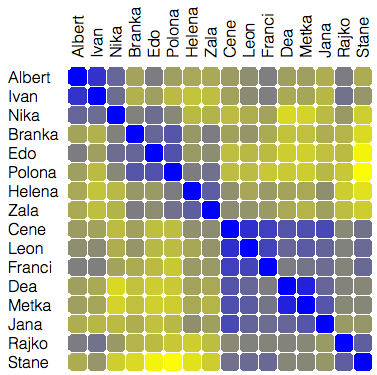
\includegraphics[width=7cm]{slike/toplotna-karta.png}
\caption{Vizualizacija podobnosti oziroma različnosti med primeri s
  tabele~\ref{t-eksterci}.}
\label{f-toplotna-karta}
\end{center}
\end{figure}

\section{Ocenjevanje razdalj med skupinami}

Tudi med skupinami primerov lahko merimo razdaljo. A tu naletimo na
problem, saj so sedaj skupine podane z množico primerov. Med primeri
znamo meriti razdalje, med skupinami pa (še) ne. Razdaljo bomo merili
med dvemi skupinami primerov, $C_u$ in $C_v$. Predpostavimo najprej,
da si skupine ne delijo primerov, torej $C_u\cap
C_v=\emptyset$. Uvedimo nekaj možnih razdalj:
\begin{itemize}
\item Razdalja med skupinama $C_u$ in $C_v$ je razdalja med njunima
  najbližjima primeroma $a\in C_u$ in $b\in C_v$ \angl{single
    linkage}:
$$d_{\rm min}(C_u, C_v)=\min_{a,b}\{d(a,b)\ |\ a\in C_u, b\in C_v\}$$
\item Razdalja med skupinama $C_u$ in $C_v$ je razdalja med njunima
  najbolj oddaljenima primeroma $a\in C_u$ in $b\in C_v$
  \angl{complete linkage}:
$$d_{\rm max}(C_u, C_v)=\max_{a,b}\{d(a,b)\ |\ a\in C_u, b\in C_v\}$$
\item Razdalja med skupinama $C_u$ in $C_v$ je povprečna razdalja med
  vsemi pari primerov iz teh dveh skupin \angl{average linkage}, torej:
$$d(C_u, C_v)={\sum_{a\in C_u}\sum_{b\in C_v}  \frac{d(a,b)}{|C_a||C_b|}} $$
\item Wardova razdalja, ki privzame, da je za vsako skupino $C$ znan
  njen centroid $R$ oziroma točka v središču skupine. Naj bo $R_u$
  centroid skupine $C_u$, $R_v$
  centroid skupine $C_v$, $R_{uv}$ pa centroid združene skupine
  $C_{uv}=C_u\cup C_v$. Potem je Wardova razdalja določena kot:
$$d_w(C_u, C_v)=\sum_{x\in C_{uv}}d(x, R_{uv})^2 - (\sum_{x\in
    C_u}d(x, R_u)^2 + \sum_{x\in C_v}d(a, R_v)^2)$$
\end{itemize}

\section{Hierarhično razvrščanje v skupine}

Postopek, ki iz podatkov razvije hierarhijo skupin, kjer je najnižje v
hierarhiji vsak primer predstavljen s svojo skupino, najvišje v
hierarhiji pa tvori skupino kar celotna množica učnih primerov, se
imenuje hierarhično razvrščanje v skupine.

\subsection{Algoritem}

Hierarhično razvrščanje v skupine najlažje opišemo kar s psevdokodo:
\begin{itemize}
\item vsak primer naj tvori svojo skupino, $C_i=\{x^{(i)}\}$,
  $x^{(i)}\in\mathcal{U}$
\item ponavljaj, dokler ne ostane ena sama skupina
\begin{itemize}
\item poišči najbližji si skupini $C_a$ in $C_b$,
  $d(C_a,C_b)=\min_{u,v}d(C_u,C_v)$
\item združi skupini $C_a$ in $C_b$ v skupino $C_{ab}=C_a\cup
  C_b$
\item nadomesti skupini $C_a$ in $C_b$ s skupino $C_{ab}$
\item izmeri razdaljo med novo skupino $C_{ab}$ in ostalimi skupinami
\end{itemize}
\end{itemize}

Prostorska kompleksnost tega algoritma je $O(m^2)$, kjer je $m$
število primerov oziroma velikost učne množice. Časovna kompleksnost
pa je $O(m^3)$ saj se algoritem izvede v $m$ korakih, v katerih mora
osvežiti in uporabiti matriko razdalj velikosti $m^2$. Z malo truda se
da postopek izračunavanja novih razdalj spisati tako, da ima manjšo
zahtevnost in je potem zahtevnost celotnega algoritma
$O(m^2\log(m))$. Tudi to ni malo. Predstavljajte si, da morate
algoritem pognati na vseh uporabnikih nekega večjega mobilnega
operaterja. Ali pa na vseh uporabnikih družabnega omrežja. Kam
shranite matriko razdalj med pari primerov? Je opisani postopek tudi
časovno zahteven?

\subsection{Dendrogram}

Postopek združevanja v skupine in rezultat tega postopka ---
hierarhijo skupin, lahko ponazorimo v drevesnem izrisu ali dendrogramu
(gr. {\em dendron} pomeni drevo, {\em gramma} pa risba). Dendrogram
hierarhičnega razvrščanja v skupine podatkov s tabele~\ref{t-eksterci}
prikazuje slika~\ref{f-dendrogram}. Dendrogram je izrisan od leve
proti desni. Stičišča skupin so od desnega roba odmaknjena skladno z
razdaljo med skupinami. Pred izvedbo postopka razvrščanja v skupine
orodja podatke tipično normalizirajo, tako da so po normalizaciji
povprečne vrednosti atributov enake nič in njihove standardne
deviacije enake 1.

\begin{figure}[htbp]
\begin{center}
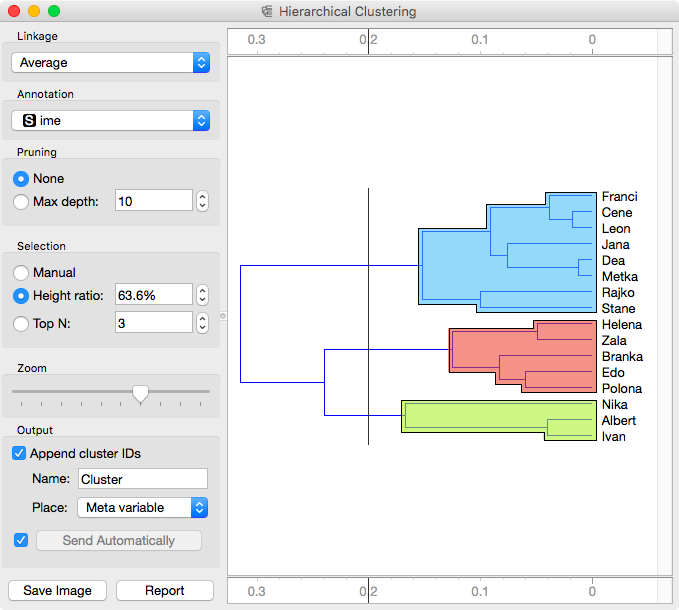
\includegraphics[width=10cm]{slike/dendrogram.png}
\caption{Primer dendrograma, kot ga izriše ustrezna komponenta v
  programu Orange. Uporabnik se je tu odločil, da dendrogram odreže v
  točki, ki primere razdeli v tri skupine. Primerna razdelitev v
  tem primeru bi lahko bila ta, ki uporabi dve skupine. Zakaj?}
\label{f-dendrogram}
\end{center}
\end{figure}

\subsection{Razlaga skupin}

Dendrogram s slike~\ref{f-dendrogram} nakazuje na tri skupine, ki smo
jih v odkrili v podatkih. Zanima nas, kaj je značilnega za posamezne
skupine. Preprosta tehnika, ki jo lahko uporabimo je, da za vsak
skupino primerjamo povprečno
vrednost posameznega atributa s povprečno vrednostjo tega atributa v
celotni učni množici. Naj bo Albert v skupini, ki jo označimo z
vrstnim številom 1, Branka v skupini 2, Cene pa v skupini 3. Povprečne
vrednosti učne množice prikazuje tabela~\ref{f-povp-skupin}.

\begin{table}[htbp]
\caption{Povprečne vrednosti percentilov pri posameznih predmetih v
  učni množici in odkritih skupinah.}
\label{f-povp-skupin}
\begin{center}
\begin{tabular}{lrrrrrrrrr}
\toprule
 & slo & ang & zgo & geo & mat & bio & fiz & kem & tel \\
\midrule
$\mathcal{U}$ & 54 & 78 & 40 & 47 & 62 & 52 & 62 & 61 & 47 \\
skupina 1 & 41 & 70 & 36 & 29 & 33 & 23 & 31 & 30 & 98 \\
skupina 2 & 92 & 96 & 80 & 95 & 45 & 58 & 45 & 42 & 44 \\
skupina 3 & 35 & 69 & 16 & 24 & 83 & 58 & 84 & 85 & 29 \\
\bottomrule
\end{tabular}
\end{center}
\end{table}

Zanima nas pravzaprav odstopanje od povprečnih vrednosti atributov
učne množice. Tu bi se sicer morali poigrati s statistiko, in
ugotoviti, katera odstopanja so značilna in kako daleč so od takih, ki
bi jih dobili iz naključne razvrstitve. Zaradi enostavnosti, ki pa bo
prav tako čisto primerna za naš primer, se tu raje zatečemo
k veliko preprostejši rešitvi. Za vsako skupino označimo odstopanja
navzdol za več kot 10 odstotnih točk z ``$-$'', in podobna odstopanja
navzgor s ``+''. 

\begin{table}[htbp]
\caption{Odstopanja ($\pm 10$ točk) od povprečnih vrednosti v učni množici.}
\label{f-odstopanja-skupin}
\begin{center}
\begin{tabular}{lcccccccccc}
\toprule
 & slo & ang & zgo & geo & mat & bio & fiz & kem & tel \\
\midrule
skupina 1 & $-$ &  &  & $-$ & $-$ & $-$ & $-$ & $-$ & + \\
skupina 2 & + & + & + & + & $-$ &  & $-$ & $-$ &  \\
skupina 3 & $-$ &  & $-$ & $-$ & + &  & + & + & $-$ \\
\bottomrule
\end{tabular}
\end{center}
\end{table}

Rezultat prikazuje tabela~\ref{f-odstopanja-skupin}. Albert, Ivan in
Nika so kot kaže športniki. Njihovo udejstvovanje s športom jim vzame
veliko časa, morda bi jim bilo potrebno pomagati pri naravoslovnih
predmetih, kjer jim malce škripa. Branka, Edo in ostali iz skupine 2
imajo rajši družboslovne predmete. Skupina s Cenetom, Deo in Metko pa
zanima naravoslovje. Ne bi bilo narobe, če bi se ti vpisali v kakšen
športni krožek.

\subsection{Stvari pa lahko tudi obrnemo}

Namesto skupin učencev nas bi lahko zanimale tudi skupine
predmetov. Kako? Tabelo podatkov enostavno zasukamo oziroma
transponiramo. Vse ostalo ostane isto. Rezultat je podan na
sliki~\ref{f-dendrogram-predmeti}.

\begin{figure}[htbp]
\begin{center}
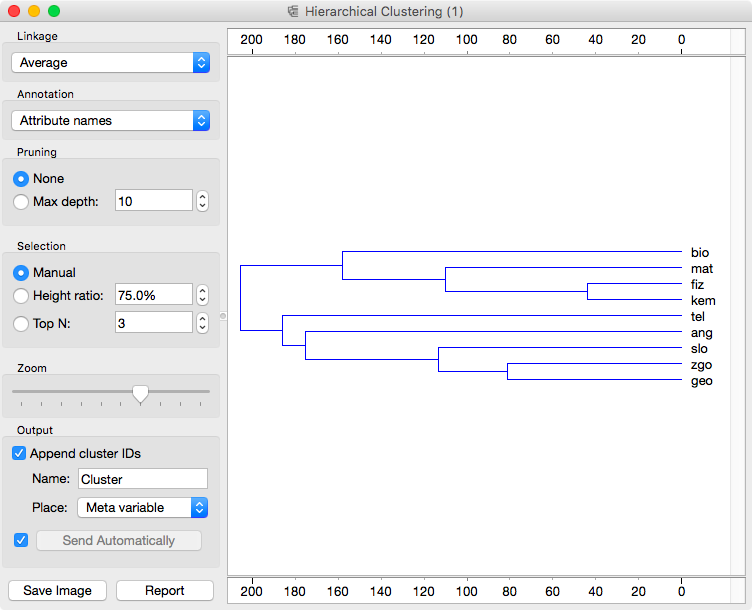
\includegraphics[width=10cm]{slike/dendrogram-predmeti.png}
\caption{Dendrogram skupin predmetov. Telovadba je nekakšen osamelec,
  samosvoj predmet precej različen od ostalih. Kako je to vidno iz
  dendrograma?}
\label{f-dendrogram-predmeti}
\end{center}
\end{figure}

\subsection{Kaj pa, ko ni skupin?}

Hierarhično razvrščanje v skupine bo vedno našlo skupine. Postopek bo
vedno razvil dendrogram, ne glede na to, ali skupine dejansko
obstajajo v podatkih ali ne. Pravzaprav, kaj pa so sploh skupine? Kako
lahko sploh ocenimo, ali te dejansko obstajajo? Tole se v tem trenutku
precej težka vprašanja in se bomo z njimi še ukvarjali. A vseeno, za
okus, naredimo naslednji poskus. Naše podatke o ocenah učencev 8.A
razreda uničimo tako, da naključno premešamo števila v vsaki od kolon,
za vsako kolono posebej. Dendrogram na takih podatkih kaže
slika~\ref{f-dendrogram-premesano}. Razdalje med posameznimi skupinami
so tu večje, stičišča povezav v dendrogramu so se premaknila proti
levi strani. Stukture, iz katere bi bile jasno razvidne skupine, ki bi
se potem združevale pri opazno večjih razdaljah kot se združujejo
primeri znotraj posameznih skupin, ni več.

\begin{figure}[htbp]
\begin{center}
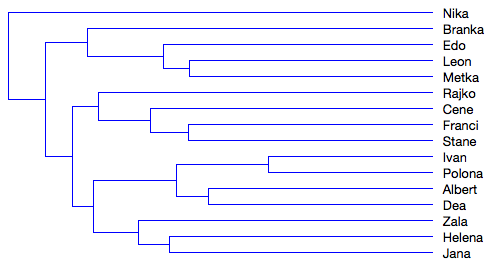
\includegraphics[width=10cm]{slike/dendrogram-premesano.png}
\caption{Dendrogram na ``ponaključenih'' podatkih. Struktura, ki bi
  nakazovala jasne skupine v podatkih, je izginila.}
\label{f-dendrogram-premesano}
\end{center}
\end{figure}

Če imamo prave podatke, te seveda ne premešamo in potem izrisujemo
``pokvarjene'' dendrograme (ali pač? a o pomenu postopkov, ki
temeljijo na ponaključenih podatkih, kdaj drugič). A je vseeno dobro
vedeti, kakšni dendrogrami so taki, kjer skupin pač ni. Torej, če
dobimo kaj podobnega, kot je dendrogram na
sliki~\ref{f-dendrogram-premesano}, je zaključek tak, da iz danih
podatkov pri dani meri razdalje in pri dani metodi za ocenjevanje
razdalj med skupinami postopek hierarhičnega razvrščanja v skupine ni
našel značilnih skupin. Prejšnji stavek je precej dolg. Krajši bi
recimo lahko samo povedal, da v podatkih ni skupin. A taka ugotovitev
ne bi bila nujno resnična. Iz naših poskusov lahko samo ugotovimo, da
če morda skupino so, jih mi pač nismo uspeli najti. Lahko pa, seveda,
da jih sploh ni.

\section{O izboru mer razdalje}

Metoda hierarhičnega gručenja ima pravzaprav dva parametra: prvi je metoda merjenja razdalj med primeri, drugi pa način določanja razdalj med skupinami. Ko imamo podatke predstavljene atributno, torej v tabeli, kjer je vsak primer predstavljen z vektorjem atributnih vrednosti, je evklidska razdalja čisto primerna mera. Če atributi izvirajo na primer iz tekstovnih podatkov in je teh veliko, se izkaže, da je pomembna ne toliko velikost posameznega vektorja kot njegova smer. Prava razdalja za take podatke je tako imenovana kosinusna razdalja. O uporabi te več v naslednjih poglavjih. Na področju biomedicine, kjer so atributi istega tipa in je bolj kot njihova vrednost pomemben vrstni red (tipa: kateri atribut je zavzel največjo vrednost, drugo največjo, ipd.) je mnogokrat uporabljana razdalja Spearmanova korelacija, ki jo izračunamo na rangi. V tem odstavku nam ni namen formalno uvesti vse te različne mere, ampak samo poudariti, da je izbor mere razdalje med primeri odvisen od problemske domene in jo določimo skladno z vedenjem oziroma intuicijo o tem, kaj res najbolj primerno določa razdaljo med primeri.

Malce drugače je z izborom pristopov merjenja razdalje med skupinami. Kot smo že zapisali, ti pristopi (npr. {\em single linkage}, {\em complete linkage}) agregirajo pare razdalj med primeri v dveh različnih skupinah. V splošnem, če ne poznamo podatkov ali pa njihovih projekcij v nižje dimenzije, bo primerna izbira povprečne razdalje \angl{average linkage}, mnogokrat pa presenetljivo dobro deluje Wardova razdalja. Po drugi strani je pristop z minimalno razdaljo \angl{single linkage} v splošnem neuporaben, razen za res posebne primere (slika~\ref{f-single-linkage}).

\begin{figure}[htbp]
\begin{center}
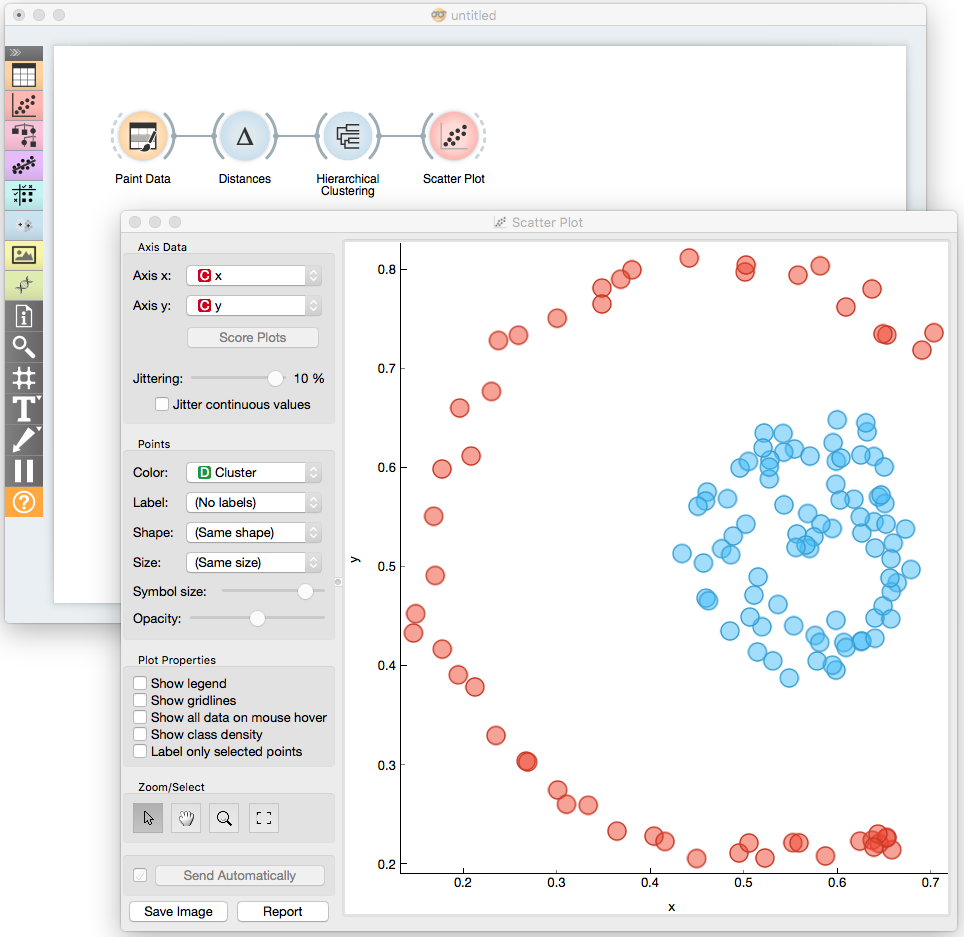
\includegraphics[width=10cm]{slike/single-linkage.png}
\caption{Primer dvodimenzionalnih podatkov in njihove razvrstitve, kjer je ustrezna metoda minimalne razdalje za merjenje podobnosti med skupinami, in kjer ostale metode merjenja razdalj odpovedo (za merjenje razdalj med primeri smo uporabili Evklidsko razdaljo).}
\label{f-single-linkage}
\end{center}
\end{figure}

Recepta, katere mere razdalj uporabiti, v zgodnjih dveh odstavkih nismo zapisali. Ker tega ne znamo. Namreč, vse je odvisno od podatkov. Ker na področju razvrščanja v skupine nimam prav dobrih mer o tem, kako dober je rezultat razvrščanja, se avtomatizacija iskanja najbolj ustreznih parametrov ne obnese najbolje. Z drugimi besedami: v splošnem ne znamo spisati enačbe, s katero bi numerično ocenili kvaliteto nastalih skupin. Ker te enačbe ni, ne moremo strojno primerjati rešitve med sabo. Ostane nam, da se zanesemo na intuicijo in na pregled rešitve s strani domenskega eksperta. Gručenje, ki je uporabniku koristno (za karkoli že), je potem tisto, za katero se na koncu odločimo.

\chapter{Metoda voditeljev}

Velika prednost metode hierarhičnega gručenja, ki smo jo spoznali v prejšnjem poglavju, je odkrivanje strukture skupin v podatkih, ki jih lahko enostavno ponazorimo v vizualizaciji imenovani dendrogram. Na podlagi te vizualizacije lahko potem (intuitivno) presojamo o kvaliteti gručenja ter se odločamo o tem, na koliko skupin bomo razbili podatke. Zanimiva je tudi uporaba te tehnike pri interaktivni analizi podatkov v orodjih, ki nam take vizualizacije ponujajo in kjer lahko gradimo delokroge \angl{workflows}, s katerimi lahko izbrane skupine nadalje opišemo in interpretiramo.

A pri tem naletimo na največjo pomankljivost hierarhičnega gručenja: metoda deluje samo na relativno majhnih množicah podatkov. Če imamo podatkov veliko, recimo nekaj deset tisoč ali pa celo milijon, hierarhično gručenje zaradi časovne in prostorske kompleksnosti odpove, dendrogram pa postane prevelik in neuporaben.

Rešitev, ki dobro deluje na velikih množicah podatkov je postopek, ki ga imenujemo metoda voditeljev \angl{$K$-means}. Seveda zastonj kosila tudi tu ni. V svoji
osnovni inačici metoda voditeljev predpostavlja, da je uporabnik v naprej določil število skupin,
na katero želi razbiti učno množico primerov. Algoritem uporablja
t.im. voditelje oziroma primere, ki določajo te skupine oziroma so
središča skupin. Postopek iskanja optimalnega razbitja je potem
naslednji:

\begin{itemize}
\item prični s $K$ naključno izbranimi voditelji $\mathcal{V}=\{v^{(i)};\ i\in{1\ldots K}\}$
\item {\bf ponavljaj}
\begin{itemize}
  \item določi razvrstitev $\mathcal{C}$ tako, da vsak primer prirediš
    najbližjemu voditelju
  \item novi voditelji naj bodo centroidi $R(C_i)$ skupin $C_i\in\mathcal{C}$, $v^{(i)}\leftarrow R(C_i)$
\end{itemize}
\item {\bf dokler} se lega voditeljev spreminja
\end{itemize}

Voditelji \angl{centroids} so navadno kar geometrijska središča primerov skupine:

$$ R(C_i) = {1\over |C_i|} \sum_{x\in C_i}x $$

Izračun teh je za zvezne atribute preprost. Ker moramo v vsaki iteraciji izračunati razdaljo do $K$ voditeljev, je časovna kompleksnost tega algoritma le linearno odvisna od števila primerov, to je $O(I*k*m)$, kjer je $I$ število iteracij. Algoritem tipično hitro konvergira h končni rešitvi. Za srednje velike probleme (npr. nekaj 1000 primerov) je lahko potrebnih manj kot 100 iteracij.

Potek optimizacije za podatke, ki so bili opisani z dvema zveznima atributoma in so vključevali 780 primerov, je prikazan na sliki~\ref{f-kmeans-trace}. Za prikazano optimizacijo je zanimivo tudi število primerov, ki so pri posameznih iteracijah spremenili svojega voditelja:
%
\begin{verbatim}
Iteration: 1, changes: 54
Iteration: 2, changes: 21
Iteration: 3, changes: 18
Iteration: 4, changes: 18
Iteration: 5, changes: 18
Iteration: 6, changes: 29
Iteration: 7, changes: 63
Iteration: 8, changes: 131
Iteration: 9, changes: 64
Iteration: 10, changes: 6
Iteration: 11, changes: 0
\end{verbatim}
%
Optimizacija se skoraj ulovi v lokalni minimum, potem pa se v osmi
iteraciji pobere in poišče rešitev, ki se nam v tem primeru zdi smiselna.

\begin{figure}[htbp]
\begin{center}
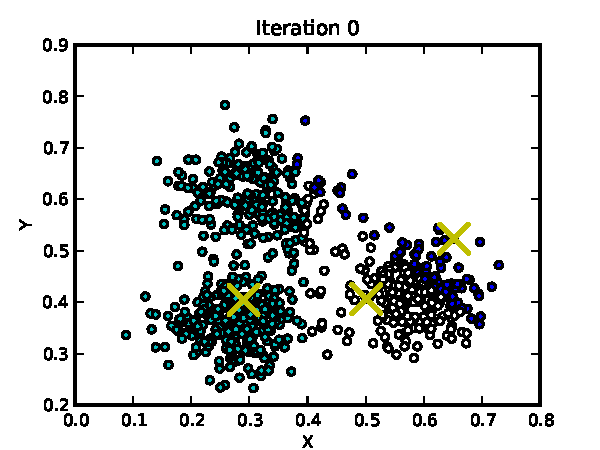
\includegraphics[width=5cm]{slike/kmeans-scatter-000.pdf}
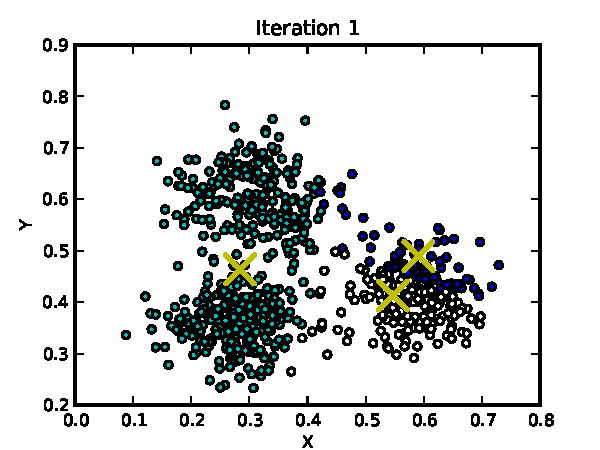
\includegraphics[width=5cm]{slike/kmeans-scatter-001.pdf}
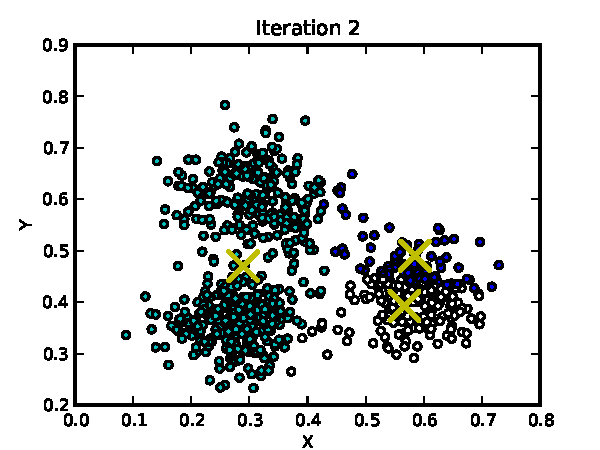
\includegraphics[width=5cm]{slike/kmeans-scatter-002.pdf}
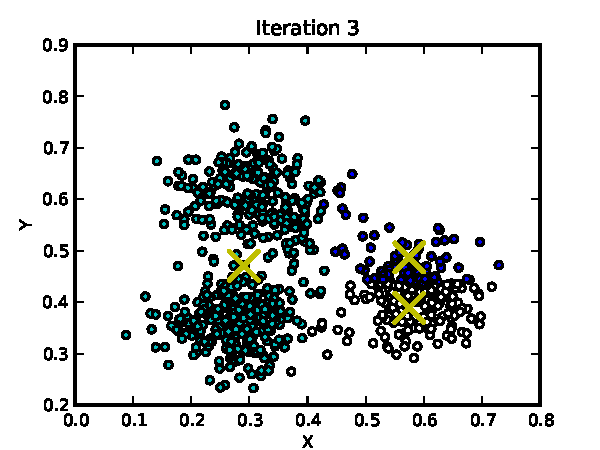
\includegraphics[width=5cm]{slike/kmeans-scatter-003.pdf}
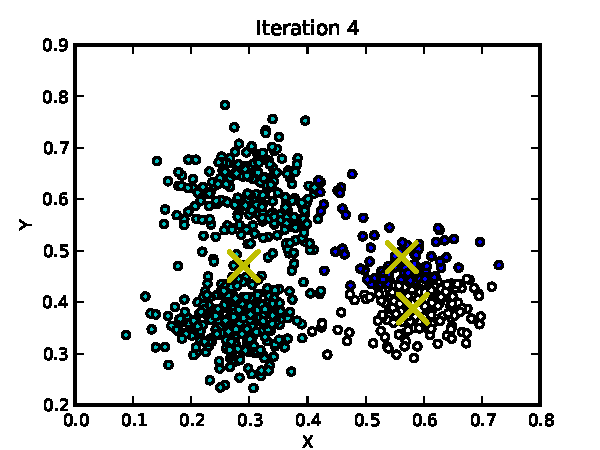
\includegraphics[width=5cm]{slike/kmeans-scatter-004.pdf}
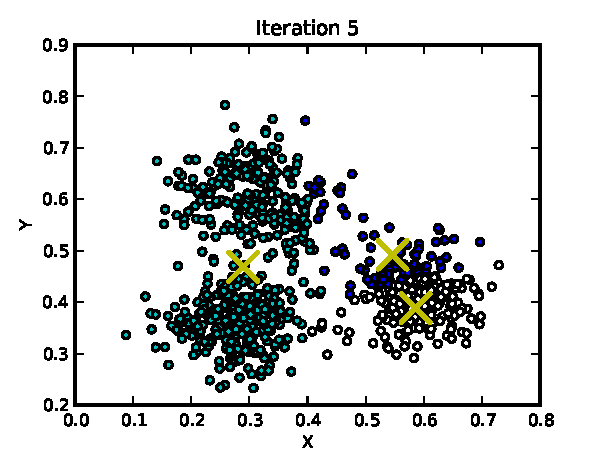
\includegraphics[width=5cm]{slike/kmeans-scatter-005.pdf}
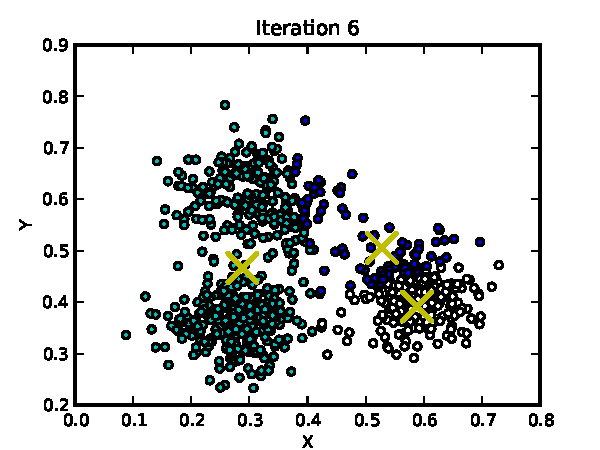
\includegraphics[width=5cm]{slike/kmeans-scatter-006.pdf}
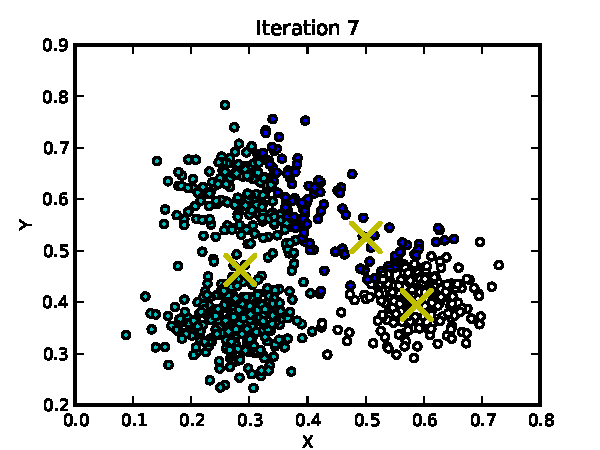
\includegraphics[width=5cm]{slike/kmeans-scatter-007.pdf}
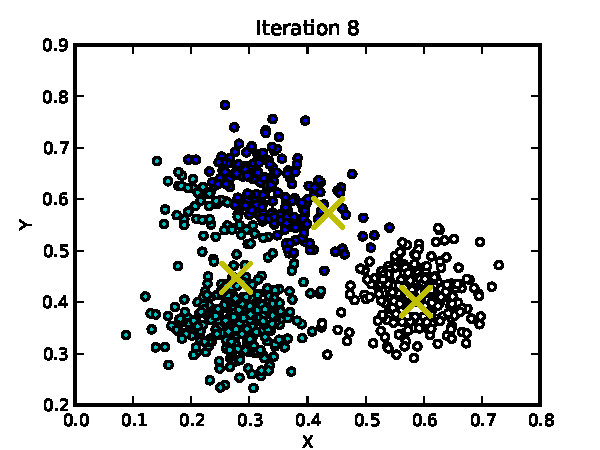
\includegraphics[width=5cm]{slike/kmeans-scatter-008.pdf}
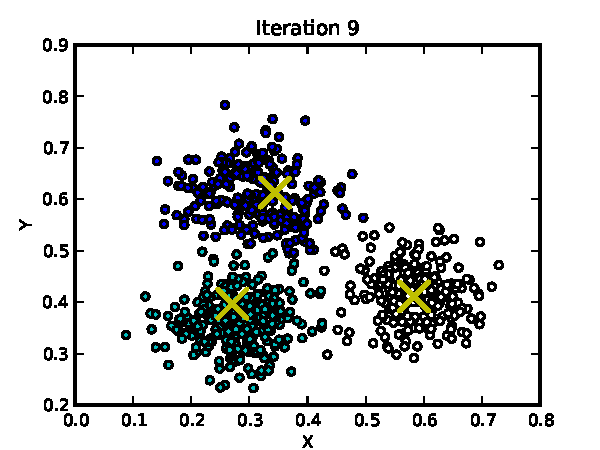
\includegraphics[width=5cm]{slike/kmeans-scatter-009.pdf}
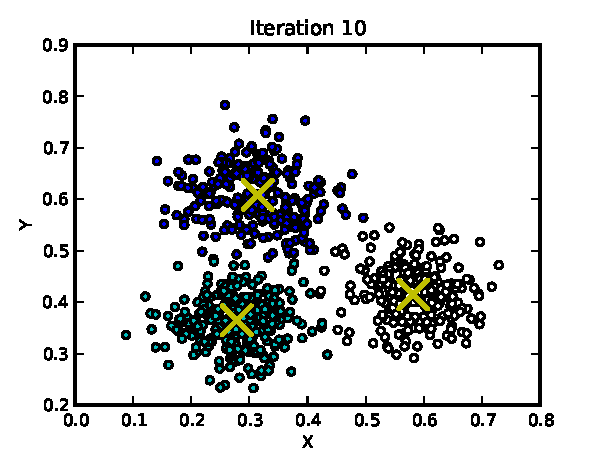
\includegraphics[width=5cm]{slike/kmeans-scatter-010.pdf}
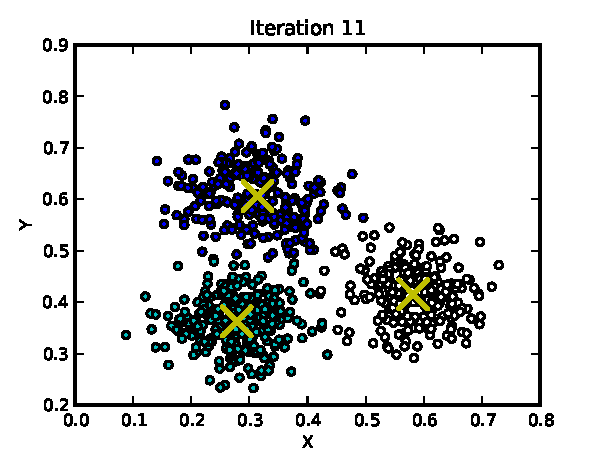
\includegraphics[width=5cm]{slike/kmeans-scatter-011.pdf}
\caption{Potek optimizacije razbitja za 780 primerov v evklidski
  ravnini. Lega voditeljev je označena s križcem. Primeri, ki
  pripadajo istemu voditelju, so označeni z isto barvo.}
\label{f-kmeans-trace}
\end{center}
\end{figure}

Tehnika voditeljev pa nas, za izbrane podatke in parametre metode,
lahko tudi preseneti in vrne nepričakovane rezultate. Primer take
razvrstitve je prikazan na sliki~\ref{f-kmeans-stripes}.

\begin{figure}[htbp]
\begin{center}
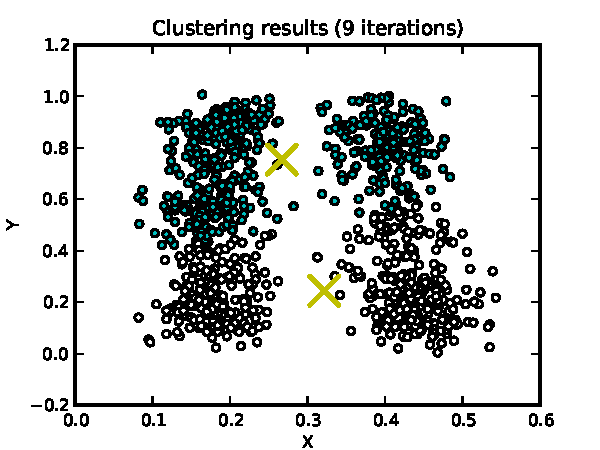
\includegraphics[width=8cm]{slike/kmeans-stripes.pdf}
\caption{Na pogled nepravilno razbitje, ki ga je predlagala metoda voditeljev.}
\label{f-kmeans-stripes}
\end{center}
\end{figure}

Rezultati metode voditeljev so lahko zelo občutljivi na izbor
primernih začetnih pogojev in mero razdalje med primeri (pri zgornjih
primerih smo uporabljali evklidsko razdaljo).

\subsection{Začetni izbor voditeljev}

Razbitje, ki ga vrne metoda voditeljev, je lahko zelo odvisna od
začetnega izbora voditeljev. Od te bo tudi odvisno število iteracij,
ki so potrebne, da postopek privedejo v stabilno stanje, v katerem so
izpolnjeni ustavitveni pogoji. Zato je smiseln študij tehnik, ki bi
voditelje izbrala čim bolje. Znanih je nekaj standardnih prijemov:

\begin{description}
\item[Naključni izbor voditeljev.] Za tega smo sicer že povedali, da
  lahko privede v neoptimalno razbitje. A se lahko temu izognemo, če
  postopek ponovimo večkrat in med poiskanimi razbitji izberemo
  najboljše. \comment{Kako to storimo? Katero razbitje je najboljše?}
\item[Izbor razpršenih voditeljev.] Poiščemo primer, ki je najbolj
  oddaljen od drugih. Naj bo to naš prvi voditelj. Potem poiščemo
  primer, ki je njemu najbolj oddaljen. To je drugi
  voditelj. Naslednje voditelje poiščemo tako, da so ti najbolj
  oddaljeni od voditeljev, ki smo jih že določili.
\item[Uporaba hierarhičnega razvrščanja.] Na podmnožici točk s
  hierarhičnim razvrščanjem poiščemo $K$ skupin in njihova
  središča uporabimo kot začetne voditelje. \comment{Zakaj ne
    uporabimo celotnega nabora primerov?}
\end{description}

\subsection{Ustavitveni kriterij}

V osnovnem algoritmu za iskanje razbitij po metodi voditeljev
zahtevamo, da se postopek ustavi šele takrat, ko se razbitje več ne
spreminja. Takrat noben primer ne zamenja svojega centroida. V
splošnem temu pogoju ne moremo vedno zadostiti, saj se nam lahko
zgodi, da pride do oscilacij in se postopek na omenjeni način nikoli
ne zaustavi. A so ti primeri v praksi zelo redki. Pri velikih množicah
primerov, in v izogib nestabilnosti, lahko namesto popolne stabilnosti
rešitve postopka zahtevamo, da se ta izteče, ko v iteraciji samo nekaj
(na primer 10) primerov ali manj zamenja skupino.

\subsection{Ocenjevanje kvalitete razbitij}

Glavna pomanjkljivost metode voditeljev, tudi z ozirom na tehniko
hierarhičnega razvrščanja v skupine, je potreba po izboru števila
skupin $K$. Uporabnik le redkokdaj ve, na koliko skupin bi bilo
potrebno rezultate razbiti. Pravzaprav je prav ``pravo'' število
skupin ena od ključnih informacij, ki bi jih radi na podlagi podatkov
ocenili.

Tu se zatečemo k razmisleku o cilju razbitja podatkov na skupine. V
splošnem bi želeli poiskati taka razbitja, kjer so si primeri znotraj
skupine čim bolj podobni, ter primeri iz različnih skupin čim bolj
različni. Če razmišljamo samo o prvem, potem želimo, da metoda
voditeljev poišče tako razbitje, kjer bo vsota oddaljenosti od
pripadajočih voditeljev oziroma spodnji izraz čim manjši:
%
$$ \sum_{i=1}^K \sum_{x\in Ci} d(v^{(i)}, x) $$
%
Predpostavimo, da se naši primeri nahajajo v evklidski ravnini in da imamo opravka s podatki z enim samim atributom. Razdaljo med točkami bomo merili z evklidsko razdaljo. Zgornji izraz se prevede v vsoto kvadratnih napak \angl{sum of squared errors, SSE} oziroma odstopanj od centroidov:
%
$$SSE = \sum_{i=1}^K \sum_{x\in Ci}(v^{(i)}-x)^2$$
%
Iščemo take centroide $C_k$, kjer je ta napaka najmanjša:
\begin{eqnarray}
\pd{}{v^{(k)}} & = & \pd{}{v^{(k)}}\sum_{i=1}^K\sum_{x\in C_i}(v^{(i)}-x)^2  \\
& = & \sum_{i=1}^K\sum_{x\in C_i} \pd{}{v^{(k)}}(v^{(i)}-x)^2 \\
& = & \sum_{x\in C_k} 2 (v^{(k)}-x)
\end{eqnarray}
%
\begin{equation}
\sum_{x\in C_k} 2 (v^{(k)}-x) = 0 \ \Rightarrow \ |C_k|\ v^{(k)} = \sum_{x\in C_k}
  x \ \Rightarrow \ v^{(k)} = {1 \over |C_k|} \sum_{x\in C_k}x
\end{equation}
%
kjer je $|C_k|$ število primerov v skupini $C_k$. Najboljši centroidi,
ki minimizirajo vsoto kvadratnih napak so ravno centri (središnjice)
skupin. Če bi vzeli namesto evklidske razdalje Manhattansko, bi s
pomočjo podobnega izvajanja kot zgoraj dobili, da so najbolj primerni
centri mediane točk v skupini.

Pri zgornjem izvajanju smo se osredotočili le na zmanjševanje
oddaljenosti točk v skupini od njihovih centroidov. Pravzaprav pa nas
zanima podobnost primerov znotraj skupine oziroma t.im. kohezija, ter
oddaljenost primerov med različnimi skupinami, oziroma
t.im. ločljivost. Mera kvalitete razbitja, ki uspešno združuje tako
kohezijo kot ločljivost je silhuetni koeficient, oziroma silhueta
razbitja. Izračunamo ga s sledečim postopkom:
\begin{itemize}
\item Naj bo $a_i$ povprečna razdalja primera $x^{(i)}$ do vseh ostalih primerov v njegovi skupini.
\item Za primer $x^{(i)}$ in neko skupino $C_j;\ x_i\not\in C_j$, ki   je različna od te, ki vsebuje $x_i$, izračunaj povprečno razdaljo   med $x_i$ in primeri v tej skupini. Poišči skupino $C_j$, kjer je ta   razdalja najmanjša. Imenujmo to razdaljo $b_i$.
\item Za primer $x_i$ je njegova silhueta enaka
  $s_i=(b_i-a_i)/\max(a_i,b_i)$.
\item Silhueta razbitja je enaka povprečni silhueti primerov v učni
  množici:
$$s={1 \over |\mathcal{U}|}\sum_{i=1}^{|\mathcal{U}|} s_i$$
\end{itemize}

Možne vrednosti silhuetnega koeficienta v teoriji ležijo na intervalu
med -1 do 1, v praksi pa pričakujemo, da bo za dani primer razdalja do
primerov v lastni skupini veliko manjša od razdalj do primerov v
najbližji tuji skupini, torej $a_i<b_i$ in zato $s_i>0$. V primeru, ko
so te razlike velike, je vrednost silhuete 1. Silhuete primerov lahko
izrišemo za vsako skupino. Uredimo jih od največjega do najmanjšega
(za primer, kjer smo razvrstili podatke nabora ``voting'' v tri
skupine, glej sliko~\ref{f-kmeans-silhouette-voting}). Kateri primeri so tisti, ki imajo kratko silhueto?

\begin{figure}[htbp]
\begin{center}
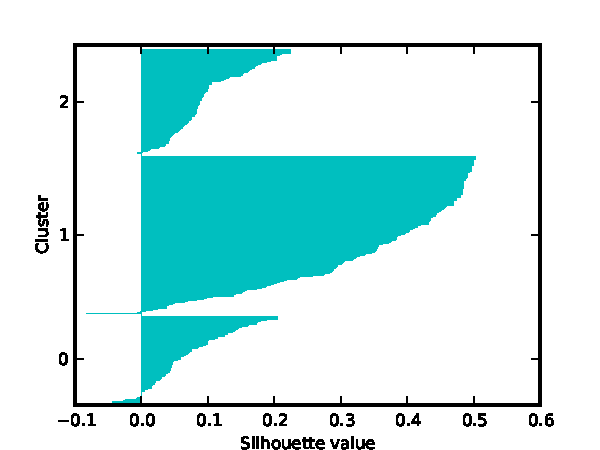
\includegraphics[width=10cm]{slike/kmeans-silhouette-voting.pdf}
\caption{Silhuete primerov iz podatkovnega nabora ``voting'' pri
  razvrstitvi v tri skupine.}
\label{f-kmeans-silhouette-voting}
\end{center}
\end{figure}

Kvaliteto razbitja za dano število skupin $K$ lahko torej ocenimo s
povprečno silhueto primerov. To nam omogoča, da ocenimo, kako primerne
so različne vrednosti $K$ (glej primer take študije s
slike~\ref{f-kmeans-silhouette-study}). Hevristika sicer ne deluje
idealno, a nam lahko, z malce previdnosti, pomaga, da izberemo
primerno število skupin za naše podatke. Previdnost je potrebna
predvsem tam, kjer so razlike med silhuetami majhne. V takih primerih
nam pomaga razmišljanje o tem, kaj posamezne skupine sploh sestavlja
in kakšne so skupne značilnosti primerov v skupinah.

\begin{figure}[htbp]
\begin{center}
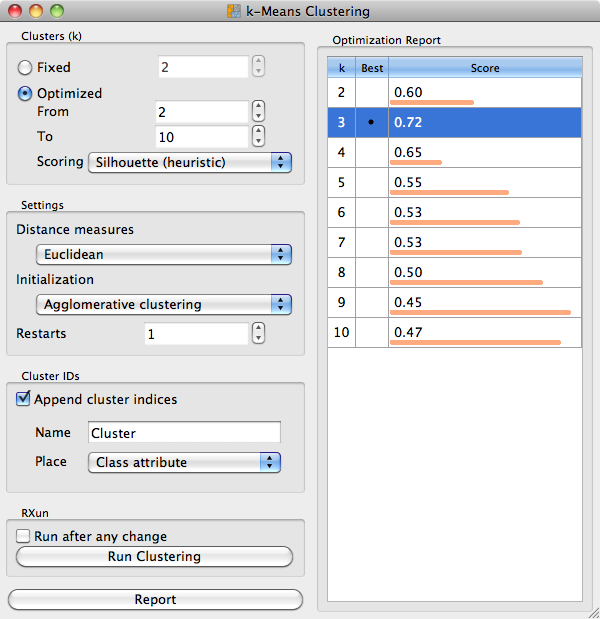
\includegraphics[width=10cm]{slike/kmeans-silhouette-study.png}
\caption{Silhuetna študija razvrstitve v različno število skupin za
  podatke s slike~\ref{f-kmeans-trace}.}
\label{f-kmeans-silhouette-study}
\end{center}
\end{figure}

\section{Kombiniranje razvrstitev in razvrščanje s konsenzom}

``Več ljudi več ve'', ali modrost množic. Tudi na področju razvrščanja
je lahko tako. Različni algoritmi, njihovi parametri ali pa rahlo
različne učne množice iz iste problemske domene nam lahko pomagajo
razkriti skupine, ki so lahko rahlo, ali pa tudi precej različne med
sabo. Bi bilo pametno, pri takem nizu razvrstitev, te skupine nekako
zliti in poiskati stabilni del razvrstitev. Če bi na primer dva
primera pri večini razvrstitev bila del istih skupin bi to bil dober
pokazatelj, da bi bilo dobro ta dva primera tudi sicer razvrstiti
skupaj. Po drugi strani pa bi lahko za dva druga primera, ki ju skoraj
nikoli nismo našli v skupnih skupinah, rekli, da pač ne sodita skupaj.

Na zgornji ideji temelji algoritem razvrščanja s
konsenzom (Monti in sod., 2003), ki ga opišemo s spodnjim algoritmom.
% \cite

\begin{tabbing}
xxx\=xxx\=xxxxxxxxxxxxxxxxxxxxxxxxxxxxxxxxxxxxxxx\=\kill
{\bf input:} \\
\> učna množica primerov $D$ \\
\> algoritem razvrščanja Cluster in izbrano število skupin $K$ \\
\> število vzorčenj $H$ \\
\\
$M\Leftarrow\emptyset$ \>\>\> množica povezovalnih matrik\\
{\bf for} $h=1,2,\ldots, H$ {\bf do} \\
\> $D^{(h)}\leftarrow {\rm Resample}(D)$ \>\> izberemo vzorec iz
učne množice \\
\> $M^{(h)}\leftarrow {\rm Cluster}(D^{(h)}, K)$ \>\> razvrstimo
primere iz $D^{(h)}$ v $K$ skupin \\
\> $M\leftarrow M\cup M^{(h)}$ \\
{\bf end} \\
$\mathcal{M}\leftarrow$ ComputeConsensusMatrix$(M)$ \\
$\mathcal{C}\leftarrow$ razbitje $D$ v $K$ skupin na podlagi $\mathcal{M}$
\end{tabbing}

Oznaka $M^{(h)}$ označuje povezovalno matriko:
$$ M^{(h)}(i,j) = \left\{
     \begin{array}{ll}
       1 & = X_i\in C\wedge X_j\in C \\
       0 & = \text{otherwise}
     \end{array}
   \right.$$
Iz množice povezovalnih matrik izračunamo matriko konsenzov:
$$ \mathcal{M}(i,j) = {\sum_h M^{(h)}(i,j) \over \sum_h
  I^{(h)}(i,j)} $$
Kjer je $I$ matrika indikatorjev, ki ima za par $i$ in $j$ vrednost 1,
če sta oba primera $X_i$ in $X_j$ prisotna v vzorcu $D^{(h)}$, sicer
pa vrednost 0. Elementi povezovalne matrike so realna števila na
intervalu od 0 do 1. Elementi ustrezajo podobnostim primerov, matrika
pa podobnostni matriki. Matrika ${\bf 1}-\mathcal{M}$ je zato matrika
razdalj med primeri, ki jo lahko uporabimo pri hierarhičnem
razvrščanju v primere ter na ta način pridobimo možne razvrstitve, ki
predstavljajo konsenz delnih razvrstitev na vzorcih iz učne množice.

\subsection{Permutacijski test}

Včasih nam tudi kvantitativna ocena, kot je silhueta, neposredno ne
pove prav dosti o tem, ali so v podatkih zares skupine ali pa je
algoritem našel neko razbitje, ki pa bi bilo podobne kvalitete tudi,
če bi bili podatki naključni oziroma, bolje, taki, kjer bi sicer
ohranili porazdelitve vrednosti posameznih atributov a izničili
interakcije med atributi. V nadaljevanju bomo zaradi poenostavitve
take podatke imenovali naključni podatki.

\begin{figure}[htbp]
\begin{center}
  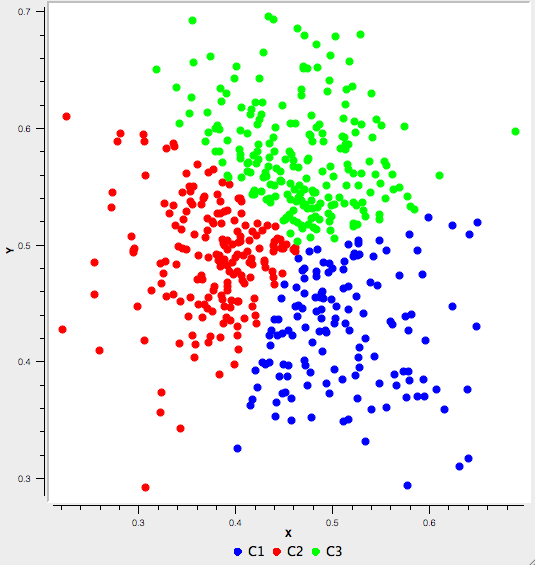
\includegraphics[width=6cm]{slike/kmeans-wrong-scatter.png}
\caption{Rezultat razbitja s tehniko voditeljev na dvoatributni domeni
izgleda lepo strukturiran, vprašanje pa je, ali smo res odkrili tri
značilne skupine. Silhueta tega razbitja je $0.50$ in je bila le rahlo
različna od silhuete za ostala razbitja na dve do deset skupin, kjer
je bila silhueta od $0.44$ do $0.49$.}
\label{f-kmeans-hairball}
\end{center}
\end{figure}


Naša hipoteza, ki jo preizkušamo in jo v statistiki imenujemo ničelna
hipoteza, je ($H_0$): silhueta $s$ ima vrednost, kot bi jo dobili,
če bi bili podatki naključni.

Zgornjo hipotezo je enostavno računsko preveriti. Generirajmo naključne
podatke. To storimo tako, da v naših podatkih za vsak atribut
naključno premešamo njihove vrednosti po primerih. Ker so podatki
podani v tabeli, je to isto, kot če vrednosti vsake kolone med sabo
premešamo. (Je to res potrebno narediti za vse kolone oziroma
atribute?) Na teh podatkih uporabimo tehniko razvrščanja in izmerimo
silhueto. To ponovimo, na primer vsaj 100-krat ali pa bolje
1000-krat. Na ta način dobimo porazdelitev vrednosti naše statistike
$s$, kot bi jo dobili, če bi ta izhajala iz naključnih
podatkov. Izmerimo sedaj to isto statistiko na nepremešanih,
originalnih podatkih in jo primerjamo z ničelno porazdelitvijo.

Zgornji postopek smo uporabili na podatkih, ki so bili podobni tem iz
slike~\ref{f-kmeans-hairball}. Za oceno ničelne porazdelitve smo
izračunali $200$ silhuet, vsakič na podatkih s premešanimi vrednostmi
atributov. Ugotovimo, da je kar $23\%$ vseh vrednosti iz ničelne
distribucije večje od naše opazovane statistike na originalnih
podatkih. Če bi trdili, da je naša ničelna hipoteza $H_0$ napačna, bi
na podlagi naših eksperimentov verjetnost napačne zavrnitve te
hipoteze bila $p=0.23$. V statistiki je to veliko prevelik prag za
zavrnitev ničelne hipoteze. Tipično je sprejemljiva meja tega praga
enaka $\alpha=0.01$, včasih celo $\alpha=0.05$. 

\begin{figure}[htbp]
\begin{center}
  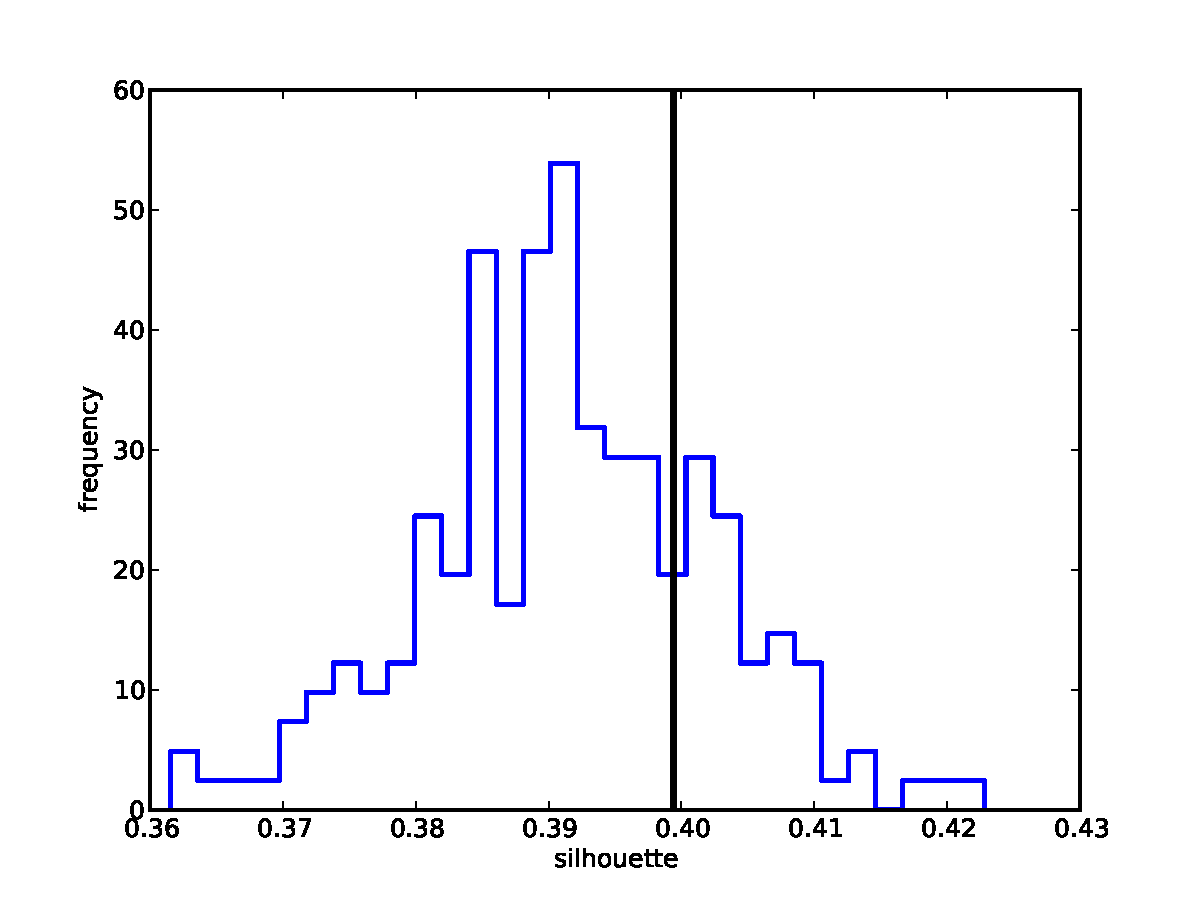
\includegraphics[width=10cm]{slike/kmeans-permutations.pdf}
\caption{Porazdelitev silhuet na permutiranih podatkih in projekcija
  (ravna črta) silhuete na originalnih podatkih kaže na to, da, vsaj
  za izbrano število skupin, za te podatke nismo našli smiselnega razbitja.}
\label{f-kmeans-permutations}
\end{center}
\end{figure}

Za konec si poglejmo še malce drugačne podatke
(slika~\ref{f-kmeans-two-overlap}). Tu so rezultati smiselni oziroma
tako vsaj zgledajo. Podatki dejansko nakazujejo, da bi lahko imeli
dve skupini. To preverimo s permutacijskim testom
(slika~\ref{f-kmeans-permutations-two}). Ničelno hipotezo zavrnemo z
verjetnostjo, da smo se pri tem zmotili $p=0.025$.

\begin{figure}[htbp]
\begin{center}
  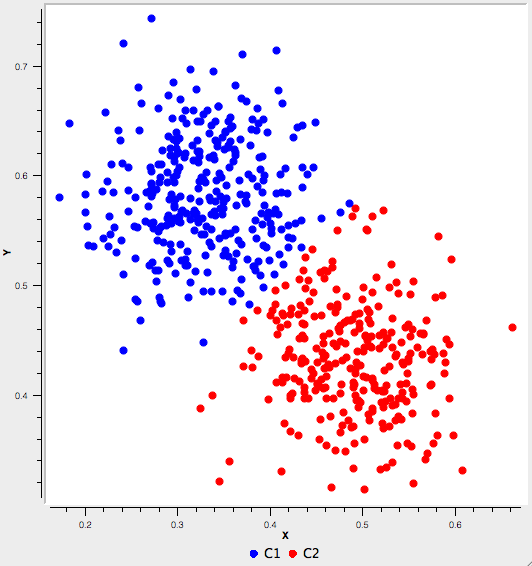
\includegraphics[width=6cm]{slike/kmeans-two-overlap.png}
\caption{Rezultat razbitja je tu morda smiseln. Silhueta za $K=2$ je
  0.68, za ostale vrednosti $K$ pa pod 0.56. Rezultate bi bilo dobro
  preveriti s permutacijskim testom.}
\label{f-kmeans-two-overlap}
\end{center}
\end{figure}

\begin{figure}[htbp]
\begin{center}
  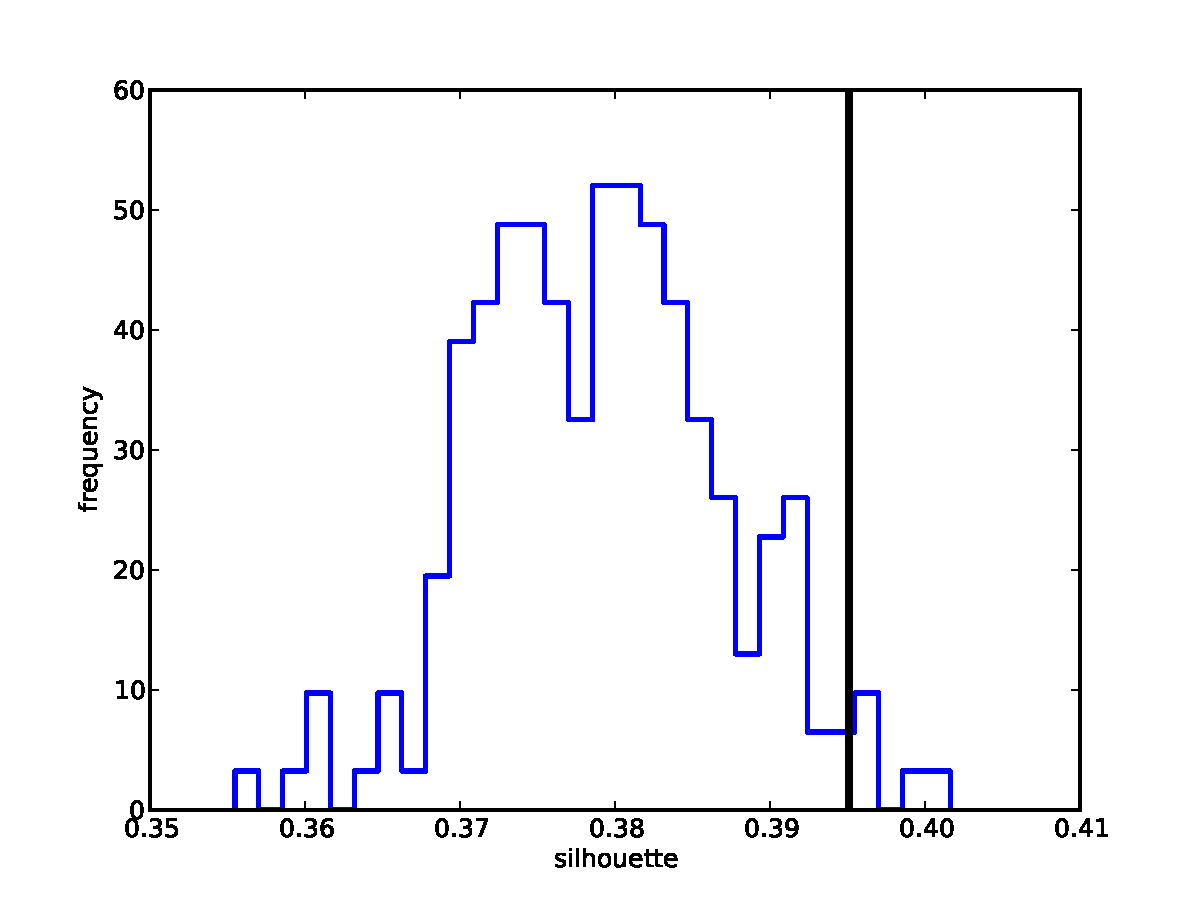
\includegraphics[width=10cm]{slike/kmeans-permutations-two.pdf}
\caption{Porazdelitev silhuet na permutiranih podatkih in projekcija
  (ravna črta) silhuete na originalnih podatkih s slike~\ref{f-kmeans-two-overlap}.}
\label{f-kmeans-permutations-two}
\end{center}
\end{figure}

\section{Predobdelava podatkov}

Do tu smo predpostavili, da imajo atributi v naši podatkovni množici
isto, zvezno, zalogo vrednosti. Taka lastnost podatkov je med temi, ki
jih uporabljamo pri reševanju praktičnih problemov, le redka. Navadno
z atributi zapišemo različne lastnosti primerov, ki nastopajo v
različnih merskih enotah. Na primer dolžina, teža, višina, ocena v
neki ocenjevalni lestvici, pa rezultati na različnih testih, in
podobno. Mere razdalje, kot je Evklidska, ne ločijo med različnimi
merskimi lestvicami, zato je potrebno podatke spremeniti tako, da bodo
vrednosti atributov med seboj primerljive. To storimo z
normalizacijo. In sicer, za vsak atribut $j$ določimo najprej njegovo
povprečno vrednost:
%
$$ \mu_j=E[X_j]={1\over N}\sum_{i=1}^N X_{ij}$$
%
kjer je $X_{ij}$ vrednost $j$-tega atributa za $i$-ti primer. Podobno
določimo tudi standardni odklon atributa:
%
$$ \sigma_j=\sqrt{E[(X_j-\mu_j)^2]}=\sqrt{{1\over N} \sum_{i=1}^N
  (X_{ij}-\mu_j)^2}$$
Podatke zdaj normaliziramo tako, da so nove vrednosti v tabeli
podatkov $Z_{ij}$ enake:
$$ Z_{ij}={X_{ij}-\mu_j\over\sigma_j} $$

\chapter{Razvrščanje besedil}

V prejšnjih dveh poglavjih so predlagane tehnike razvrščanja
predpostavljale, da lahko razdaljo, ali pa podobnost med primeri
enostavno izračunamo. Vsi naši primeri so bili opisani atributno in
razdalja je bila lepo določena z, na primer, razdaljo v evklidskem
prostoru. Podatke smo morali predobdelati in vsakega od
atributov normalizirati, drugih, bolj kompleksnih priprav podatkov pa
postopki razvrščanja niso zahtevali.

Drugače je s tekstovnimi dokumenti, ali besedili. Vzemimo na
primer, da moramo v skupine urediti naslednje tri novice:

{\small
\begin{quotation}
Na odru ljubljanske Drame se drevi ustavlja prva slovenska godba na pihala, ki že več kot 15 let preigrava skoraj izključno ulični džez New Orleansa. Cerkljanski Kar Češ Brass Band, ki neworleanški džez interpretira na svojevrsten in svež način, so v gledališče povabili v sklopu cikla Drama Akustika.
\end{quotation}

\begin{quotation}
Tretji oktobrski konec tedna na Ravnah na Koroškem zdaj že tradicionalno poteka Festival slovenskega jazza, katerega spremljajoči dogodki se na Koroškem vrstijo že od septembra. Tridnevni festivalski vrhunec je v Kulturnem centru Ravne odprl Big Band RTV Slovenija z vsestranskim glasbenikom Boštjanom Gombačem.
\end{quotation}

\begin{quotation}
Murskosoboški policisti so 33-letniku z območja Murske Sobote zasegli
posušeno konopljo, sadike in gotovino, za katero sumijo, da jo je
dobil s preprodajo. Pri tem so v hiši osumljenega odkrili poseben
prostor za gojenje konoplje pod umetno svetlobo. V tem prostoru so
našli in zasegli tudi 20 sadik konoplje, visokih do 90 centimetrov, in
dober kilogram posušene oz. delno posušene konoplje.
\end{quotation}
}

Nam, ljudem, je ta razvrstitev enostavna. Zadnja, tretja novica, sodi
v črno kroniko, prvi dve pa med kulturne novice.

Programsko razvrščanje novic s tehnikami iz prejšnjega poglavja pa ni
trivialno. Očitno bomo morali določiti nove mere, ki nam bodo pomagale
oceniti, kako različna so si med sabo besedila. Pristopi k razvrščanju
dokumentov, ki jih predlagamo v tem poglavju, temeljijo na
preoblikovanju besedil v atributno obliko, kjer je moč take mere
določiti, da bi nato za razvrščanje uporabili tehnike, kot sta
hierarhično razvrščanje v skupine in metodo voditeljev, ki jih že
poznamo.

\section{Elementi predstavitve besedilnih dokumentov}

\subsection{$k$-terke znakov}

``Murskosoboški'' lahko predstavimo z dvojkami ``mu'', ``ur'', ``rs'',
..., torej s pari znakov, ki si sledijo v zaporedju. Za vsak par lahko
izračunamo frekvenco pojavitve v besedilu oziroma relativno frekvenco,
ki je enaka ocenjeni verjetnosti pojavitve $k$-terke. 

Število $k$-terk je veliko že za pare ($n=2$), za večje vrednosti $k$
pa jih je mnogo ali ogromno. V praksi se uporabljajo $k$-terke do
$n=5$. Zanimivo pa je, da je že porazdelitev dvojk lahko
karakteristična za posamezne jezike in lahko na podlagi teh
razpoznamo, v katerem jeziku je napisano določeno
besedilo\footnote{Glej
  \url{www.lingua-systems.com/language-identifier/lid-library/identify-language.html}}. Za
bolj zahtevne naloge je potrebno seveda uporabiti daljše $k$-terke.

Te predstavitev je načelno enostavna, a jo precej oteži uporaba
posebnih znakov, ki jih moramo ali upoštevati ali pa primerno
predobdelati besedilo.

\subsection{Besede}

Dokumente lahko predstavimo z vrečo besed \angl{bag of words}, to je s
skupino besed in številom njihovih pojavitev v dokumentu. Pri tem
lahko besedilo najprej predobdelamo:
\begin{itemize}
\item odstranimo manj pomembne besede \angl{stop-words}, ki so za
  slovenščino na primer ``in'', ``ali'', ``ter'', ipd.
\item vse besede nadomestimo z njihovimi koreni ali pa lemami. V
  računalništvu je lematizacija algoritmični postopek določevanja leme
  določeni besedi. Postopek ni enostaven in je tipično odvisen od
  jezika, v katerem je zapisano besedilo. Za angleščino je na primer
  znan Porterjev iskalnik korenov besed \angl{Porter stemmer}, ki je
  sestavljen iz ročno izdelanih pravil\footnote{Implementacija
    Porterjevega korenjenja v različnih programskih jezikih je
    dostopna na \url{http://tartarus.org/martin/PorterStemmer}}.
\end{itemize}

Predstavitev z vrečo besed zanemarja dejstvo, da je pomen besed
mnogokrat odvisen od konteksta. Ista beseda ima lahko različne pomene,
ali pa imajo isti pomen lahko različne besede. Prav tako nam taka
predstavitev ne bo mogla razrešiti problem podpomenk in drugačnih
povezav med različnimi izrazi.

Število pojavitev besed v dokumentu je seveda odvisna od dolžine
dokumenta. Da ta vpliv izničimo, namesto števila pojavitev besed
uporabljamo relativno frekvenco, to je verjetnost, da bi pri
naključnem izboru besede iz dokumenta izbrali določeno besedo.

\iffalse
Primer predobdelave besedila v programskem jeziku Python s knjižnico
iz paketa Orange je podan spodaj. Koda odstrani nepomembne besede,
ustvari seznam besed ter besedam iz tega seznama poišče leme.

\begin{python}
import orngText

def preprocess(text):
    pp = orngText.Preprocess(language='en')
    text.lower()
    text = pp.removeStopwords(text)
    tokens = pp.tokenize(text)
    lemmas = pp.lemmatize(tokens)
    
    print "Text:", text
    print "Tokens:", " ".join(tokens)
    print "Lemmas:", " ".join(lemmas)
    return lemmas

preprocess("The main point of writing a text is to convey " +
           "ideas, information, or knowledge to the reader.")
preprocess("He ensnared in an insider trading investigation " +
           "and a former director is expected to " +
           "surrender to authorities.")
\end{python}
\fi

\subsection{Fraze}

Fraze so lahko $k$-terke besed, ki se v besedilu nahajajo neposredno
druga ob drugi ali pa v bližnji okolici. Okolico lahko določa, na
primer, okno zaporedja petih besed. Težava pri tej predstavitvi je, da
je lahko možnih kombinacij že za pare besed ogromno. Pred leti je
Google objavil svojo zbirko fraz~\footnote{Glej
  \url{http://googleresearch.blogspot.com/2006/08/all-our-n-gram-are-belong-to-you.html}.},
ki jih je odkril iz besedilnih dokumentov. Vsebovala je na primer
314.843.401 pare besed, 977.069.902 trojk, 1,313,818,354 četvorčkov in
1,176,470,663 fraz s petimi besedami.

Uporaba fraz je smiselna ob souporabi fraznega korpusa, to je, baze že
znanih oziroma izbranih fraz za določeno problemsko
področje. Predstavitev z vrečo besed je načelno ustrezno moč dopolniti
s frazami iz besedila, tako da vsaka fraza tvori nov atribut.

\subsection{Besedne vrste}

Koristi nam lahko tudi prepoznavanje besednih vrst
\angl{part-of-speech}, kot so imena ljudi, krajev, organizacij. Za
prepoznavanje besednih vrst bomo morali uporabiti algoritme, ki znajo
besedilo analizirati veliko globlje in pri tem uporabljajo lingvistično
znanje ali pa vnaprej pripravljeni korpus. Seveda bo taka analiza tudi
odvisna od uporabljenega jezika. Pri katerih besedah v spodnjem
besedilu bi določitev besednih vrst lahko bila koristna pri analizi?

\begin{python}
We walk down the dirty old street.
The mailbox stood on the walk.
We heard cries echoing in the night.
The babied cries all night.
\end{python}

\subsection{Taksonomije}

V splošnem se taksonomija nanaša na stopenjsko razvrstitev
stvari. Pomaga nam pri ugotavljanju povezanosti med stvarmi, pri bolj
podrobnih taksonomijah pa iz njih zvemo še za
vrsto relacije. Primer take taksonomije za angleške besede je
WordNet~\footnote{WordNet je prosto dostopen na naslovu
  \url{http://wordnetweb.princeton.edu}.}. Odlična vizualizacija
povezav med besedami, kjer je prikazan tudi pomen povezav, je dostopna
na spletni strani Visuwords \footnote{\url{http://www.visuwords.com/}}
(slika f-visuwords). Enostavnejša oblika zapisa take taksonomije je
slovar sopomenk ali tezaver \footnote{Glej
  npr. \url{http://www.tezaver.si/}.}.

\begin{figure}[htbp]
\begin{center}
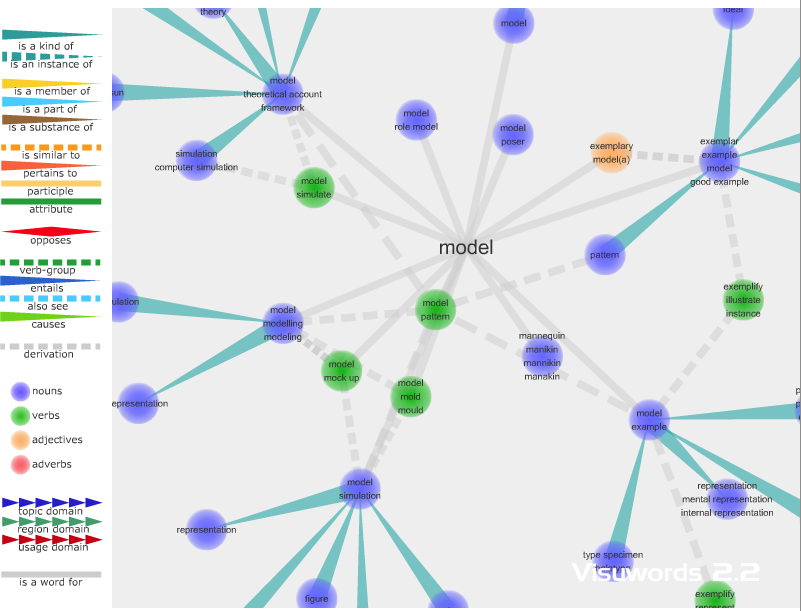
\includegraphics[width=15cm]{slike/visuwords.png}
\caption{Del taksonomije okoli angleške besede ``model'', kot jo
  prikaže spletna aplikacija Visuwords.}
\label{f-visuwords}
\end{center}
\end{figure}


\subsection{Slovnična analiza}

K računalniškem razumevanju besedila bi seveda zelo pripomogla
slovnična analiza. Uporabe tovrstnega globljega razumevanja besedila
pri razvrščanju dokumentov je predmet velikega števila trenutnih
raziskav. Prav možno je, da bodo v prihodnosti te, bolj kompleksne
jezikovne tehnologije nadomestile plitvejše, statistične tehnike ki
uporabljajo štetje parov črk ali preštevanje besed. A je prav
enostavnost slednjih in točnost, ki jo omogočajo že ti izjemno
preprosti pristopi ena od ovir za prevlado bolj kompleksnih
tehnologij.

\subsection{Uporaba pripadajočih oznak}

Mnogo dokumentov je danes označenih. Naj bodo to spletne strani
(npr. \url{del.icio.us}), dokumenti v raznih zbirkah, zapisi v
programu EverNotes, seznami bibliografskih enot v skladiščih povzetkov
CiteULike\footnote{\url{www.citeulike.org}} ali
PubMed\footnote{\url{http://www.ncbi.nlm.nih.gov/pubmed/}}. Oznake so
lahko bile prosto izbrane, ali pa vzete iz posebej za to določenega
slovarja ali pa ontologije. Dokumente lahko označujejo vsi, ki imajo
do njih dostop, ali pa samo pooblaščeni uporabniki ali kuratorji. V
vsakem primeru nam oznake lahko služijo kot osnova za predstavitev
vsebine dokumentov in zamenjujejo ali pa dopolnjujejo elemente, kot
smo jih predstavili zgoraj.

\begin{figure}[htbp]
\begin{center}
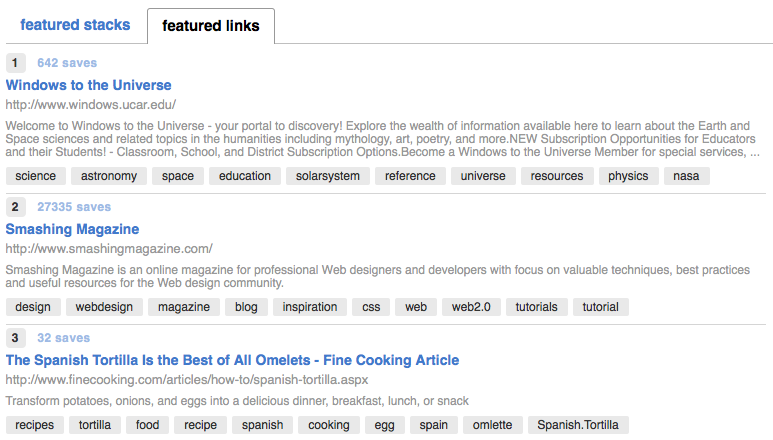
\includegraphics[width=15cm]{slike/delicious.png}
\caption{Oznake spletnih strani, kot so jih uporabniki določili v
  družabnem okolju del.icio.us.}
\label{f-delicious}
\end{center}
\end{figure}


\section{Ocenjevanje podobnosti med dokumenti}

V tem besedilu se bomo omejili na najpreprostejšo obliko predstavitve,
kjer besedilni dokument predstavimo z vektorjem enot in njihovo
frekvenco ali relativno frekvenco. Nestrukturiran dokument torej
predstavimo z atributnim jezikom. Ker je atributov lahko zelo veliko,
in ker vsi dokumenti nimajo nujno določene vse atribute, je matrika z
dokumenti v vrsticah in vrednosti atributov v kolonah zelo
prazna. Namesto te predstavitve lahko zato uporabimo slovar, z
elementi kot ključi in njihovimi frekvencami kot vrednostmi.

\subsection{Transformacija tf-idf}

Pogostost elementa (besede, terke) v dokumentu je enostavno število
pojavitev tega elementa v dokumentu. Če bi uporabljali to število, bi
prihajalo do večjih razlik med daljšimi in krajšimi dokumenti. Zato
pogostost pojavitve normaliziramo in namesto njih uporabljamo
relativne frekvence, oziroma iz dokumenta ocenimo verjetnosti
pojavitve določenega elementa. To označimo z $\mathrm{tf}(t,d)$
\angl{term frequency}.

Načelno imamo raje elemente, ki se pojavljajo v manj dokumentih in so
zaradi tega bolj specifični. Na osnovi elementov, ki se pojavijo v
večini dokumentov, bi te zelo težko razlikovali. Zato uvedemo pojem
inverzne frekvence v dokumentih \angl{inverse document frequency}, ki
jo uporabljamo kot splošno mero za pomembnost določenega elementa:
$$\mathrm{idf}(t) =  \log \frac{|D|}{|\{d: t \in d\}|}$$
kjer je $|D|$ število dokumentov v množici dokumentov $D$ in $|\{d : t
\in d\}|$ število dokumentov, ki vsebujejo element $t$ (torej, kjer je
$\mathrm{tf}(t,d) \neq 0$). Če elemente ni v korpusu, bi zgornje
vodilo k deljenju z 0. Zato lahko zgornji izraz prilagodimo in
zapišemo $1 + |\{d : t \in d\}|$.

Utež elementa $t$ v danem dokumentu $d$ je potem zmnožek njegove
frekvence v tem dokumentu in splošne pomembnosti tega elementa:
$$\mathrm{tf\mbox{-}idf}(t,d) = \mathrm{tf}(t,d) \times \mathrm{idf}(t)$$

\subsection{Kosinusna podobnost}

Čeprav bi za merjenje razdalj med vektorji, ki predstavljajo
dokumente, lahko uporabljali tudi Evklidsko razdaljo (glej prejšnje
poglavje), se ta na področju obravnave besedilnih dokumentov ne
uporablja. Razlog je preprost. Imejmo dva vektorja, $X$ in $Y$ in
predpostavimo, da sta zelo različnih velikosti, a da kažeta v isto
smer. Evklidska razdalja med njima je lahko večja kot med vektorjema,
ki bi bila kratka, a kazala v popolnoma različne smeri. Na področju
besedilnih dokumentov smer vektorja ustreza specifičnemu profilu
dokumenta v smislu vsebovanosti posameznih elementov. Pomembna je
smer, kamor kaže vektor, in manj (ali pa čisto nič) njegova
dolžina. Razliko med smerjo dveh vektorjev lahko merimo s kotom med
vektorji, ta pa je proporcionalna kosinusu kotov. Za dva vektorja
$\mathbf{a}$ in $\mathbf{b}$ velja:
$$\mathbf{a}\cdot\mathbf{b}
=\left\|\mathbf{a}\right\|\left\|\mathbf{b}\right\|\cos\theta$$
Podobnost med primeroma $X$ in $Y$ lahko zato zapišemo kot:
$$\text{sim}(X,Y) = \cos(\theta) = {X \cdot Y \over \|X\|\ \|Y\|}
= \frac{ \sum_{i=1}^{m}{X_i \times Y_i} }{
  \sqrt{\sum_{i=1}^{m}{(X_i)^2}} \times \sqrt{\sum_{i=1}^{m}{(Y_i)^2}}
}$$

\subsection{Podobnost po Jaccardu}

Kadar imamo opraviti z oznakami (torej, ne z besedami iz besedila, pri
katerih poleg vsebnosti opazujemo tudi število pojavitev) je poleg
kosinusne razdalje smiselno opazovati tudi podobnost po Jaccardu:
%
$$J(X,Y) = {{|X \cap Y|}\over{|X \cup Y|}}$$
%
Tu so dokumenti predstavljeni z množico oznak, kjer je $X \cup Y$
množica oznak uporabljena pri vsaj enem od obeh dokumentov, $X \cap Y$
pa množica oznak, ki so skupne obema dokumentoma.

\iffalse
\section{Podobnost med besedilnimi dokumenti in kompresija}

% Relativno entropijo med dvema viroma (dokumentoma) $A$ in $B$ lahko določimo
% z naključnim izborom krajšega podniza $b$ iz dokumenta $B$:
%
% $$H_{AB} = (\Delta_{Ab}-\Delta{Bb})/|b|$$
%

Naj bo $L_X$ dolžina zgoščenega dokumenta z besedilom. Torej, nek
dokument smo zgostili z ustreznim algoritmom (npr. gzip) in izmerili
dolžino zgoščenega dokumenta v bitih. Za nek niz znakov $y$ lahko
potem izmerimo, kako dobro nam zgoščevanje, ki ga je algoritem odkril
za dokument $X$, pomaga pri zgostitvi znakovnega niza $y$. Zapišimo to
oceno z $\Delta_{Xy}=L_{X+y}-L_{X}$. Razdaljo med dokumentoma $A$ in
$B$ lahko potem ocenimo z:
%
$$d(A,B) = {(\Delta_{AB}-\Delta_{BB}) \over \Delta_{BB}} +
{(\Delta_{BA}-\Delta_{AA}) \over \Delta_{AA}}$$

Spodnja koda implementacija mero podobnosti med dokumenti, ki
uporablja zgoščevanje:

\begin{python}
import Orange
import zlib

def clen(s):
    """Length of compressed string"""
    return len(zlib.compress(s, 9))

def delta(a, b):
    return clen(str(a)+str(b)) - clen(str(a))

def zip_distance(sa, sb):
    """Zip-based distance between two strings"""
    dAa = delta(sa, sa)
    dAb = delta(sa, sb)
    dBa = delta(sb, sa)
    dBb = delta(sb, sb)
    sAB = (dAb - dBb) / float(dBb) + (dBa - dAa) / float(dAa)
    return sAB

def distance(e1, e2, att="news"):
    """Return distance of two examples, assumes one text attribute"""
    return zip_distance(e1[att], e2[att])

data = Orange.data.Table("data/yahoo.tab")

ref = data[-1]
print "Most similar to:", ref["abs"]
res = sorted([(distance(ref, d), d) for d in data if not d == ref])
for (dis, d) in res[:5]:
    print "%3.1f %s" % (dis, d["abs"].native())
\end{python}

Podatki, ki smo jih uporabili pri zgornjem primeru, so bili zbrani iz
novic spletne strani yahoo (datoteka je dostopna na spletni strani
predmeta). Namenoma smo zbrali različne novice s področja športa,
znanosti in gospodarstva in za izbrano novico na podlagi izpisa pet
najbolj podobnih novic ugotavljali, ali algoritem na teh podatkih
vrača smiselne rezultate. Tako smo na primer za novico o padanju
finančnih trgov ugotovili:

\begin{python}
Most similar to: Money market falls
54.9 GM and Ford to junk status
55.1 Unlilever Q1 earnings beat forecast
55.9 Americans loose to Canada in hockey
56.0 Mars polar lander sighted
56.0 General Motors downgraded
\end{python}
\fi

\chapter{Linearna regresija}

Vinkove rezultate iz kemije so založili. Enostavno, komisija je
izgubila izpitne pole. Rešitev: Vinko bo kemijo pisal še
enkrat. Ampak, ne more, je ravno odšel na trening odbojke v
Rio. Ravnatelj pravi, da je tako ali tako vseeno, ker da eksterci ne
štejejo. Bi pa razredničarka silno želela imeti to oceno, da lahko
Vinka uvrsti v primerno učno skupino. V zbornici je učiteljica fizike
rekla, da so ocene iz kemije tako ali tako podobne tem iz fizike
(slika~\ref{f:fiz-kem-tab}). Zamrmrala je še nekaj okoli regresijskih
modelov in premic, potem pa odšla na mete Galilejeve krogle iz
strehe. Tisti dan je niso več videli.

\begin{table}[htbp]
\caption{Rezultati zunanjega preverjanja za 16 učencev razreda 8.A iz
  fizike in kemije.}
\label{f:fiz-kem-tab}
\begin{center}
\begin{tabular}{lrrrrrrrrr}
\toprule
ime & fiz & kem \\
\midrule
Albert & 46 & 36 \\
Branka & 11 & 22 \\
Cene & 100 & 89 \\
Dea & 90 & 92 \\
Edo & 17 & 12 \\
Franci & 98 & 91 \\
Helena & 81 & 94 \\
Ivan & 33 & 48 \\
Jana & 87 & 91 \\
Leon & 77 & 79 \\
Metka & 78 & 93 \\
Nika & 15 & 5 \\
Polona & 22 & 13 \\
Rajko & 51 & 52 \\
Stane & 92 & 96 \\
Zala & 92 & 67 \\
\bottomrule
\end{tabular}
\end{center}
\end{table}

Vinko je fiziko pisal 70. Razredničarka je lepo prosila za pomoč učiteljico
matematike, ki je bila tisti dan posebej razpoložena. Začnimo z
grafom, pravi. Tistim z ocenami iz fizike in kemije
(slika~\ref{f:fiz-kem}).

\begin{figure}[htbp]
\begin{center}
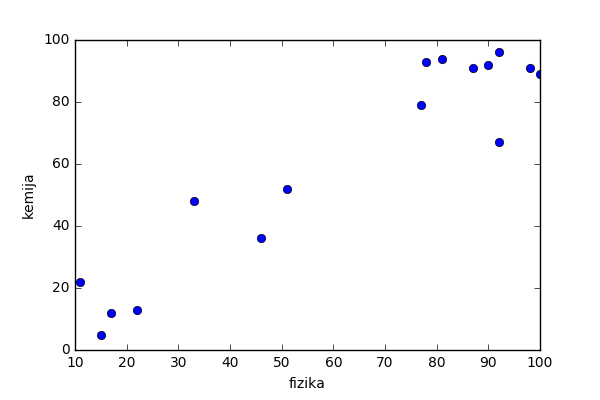
\includegraphics[width=10cm]{slike/fiz-kem.png}
\caption{Ocene fizike in kemije na razsevnem diagramu.}
\label{f:fiz-kem}
\end{center}
\end{figure}

\section{Linearni model ene spremenljivke in kriterijska funkcija}

Učiteljica fizike ima kot kaže prav, ocene kemije in fizike so med
sabo nekako povezane. Tudi učiteljica matematike ima prav: če se le
da skušamo podatke najprej predstaviti v kakšnem grafu. Od tu dalje
bomo poskušali sami. Morda začnemo s premico, ki ji bomo rekli kar
model. Model zato, ker lahko za vsako oceno pri fiziki na podlagi
modela napovemo oceno pri kemiji. Da bo vse skupaj zgledalo bolj učeno
in primerno za univerzitetni študij, označimo oceno pri fiziki s
spremenljivko $x$, oceno pri kemiji, ki jo računamo na podlagi ocene
iz fizike in jo v našem modelu modeliramo pa z $y$. Ocena kemije je
funkcija ocene iz fizike, zato lahko zapišemo:

\begin{equation}
  y = f(x)
\end{equation}

Rekli smo, da bomo zadeve poenostavili in da bo naš model kar
premica. Nekaj takega, kot kaže slika~\ref{f:fiz-kem-priblizno}. Na njej bi iz
ocene fizike 70 ocenili, da bo ocena kemije znašala 62. Ampak, ali je
premica, ki jo kaže slika, res tista ``prava''? Obstaja kakšna boljša
premica, kakšen boljši model? Kako pa sploh ocenimo kvaliteto modela?

\begin{figure}[htbp]
\begin{center}
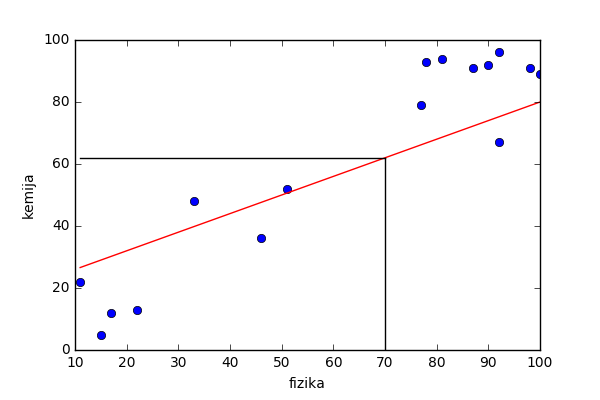
\includegraphics[width=10cm]{slike/fiz-kem-priblizno.png}
\caption{Linearni model, ki iz ocene fizike izračuna oceno za
  kemijo. Za Vinkovo oceno iz fizike 70 predvidi, da je ocena pri
  kemiji enaka 62. Pravilno?}
\label{f:fiz-kem-priblizno}
\end{center}
\end{figure}

Za vsako točko v grafu, vsak znan podatek, torej za vsak par vrednosti
$(x^{(i)},y^{(i)})$ lahko izračunamo napako, ki jo dobimo, ko vrednost odvisne
spremenljivke $y$ napovemo z modelom. Napoved označimo z $\hat{y}$ in
za primer $i$ izračunamo napako napovedi
$\epsilon^{(i)}=\hat{y}^{(i)}-y^{(i)}=f(x)-y^{(i)}$. Vse napake za naš dani model in
primere v učni množici smo označili na sliki~\ref{f:fiz-kem-eps}.

\begin{figure}[htbp]
\begin{center}
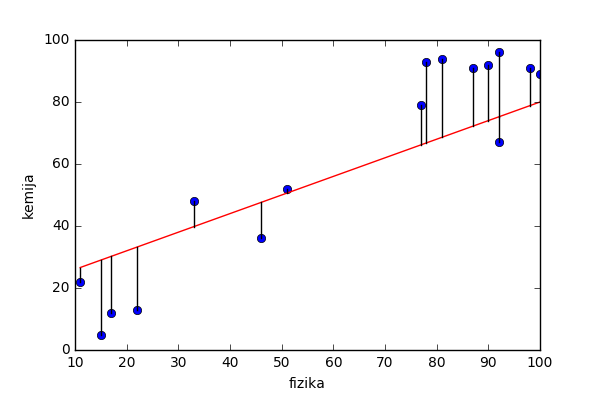
\includegraphics[width=10cm]{slike/fiz-kem-eps.png}
\caption{Napake linearnega modela na učni množici.}
\label{f:fiz-kem-eps}
\end{center}
\end{figure}

Napake $\epsilon^{(i)}$ so lahko pozitivne ali negativne.
Pravzaprav nas predznak ne zanima, zanima nas samo velikost napake. In
če že, nas ne zanimajo tiste majhne napake, ampak nas motijo predvsem
tiste večje, recimo napake pri Zali in Albertu. Radi bi, da bi naš
model bil tak, da bi napake, ki ga naredi pri napovedi primerov iz
učne množice bile čim manjše. Razmišljanje iz tega odstavka lahko
kvantificiramo, oziroma izrazimo numerično s funkcijo:

\begin{equation}
J = {1\over 2m}\sum_{i=1}^m {\epsilon^{(i)}}^2 = {1\over 2m}\sum_{i=1}^m
(\hat{y}^{(i)}-y^{(i)})^2 = {1\over 2m}\sum_{i=1}^m (f(y^{(i)})-y^{(i)})^2
\label{eq:jab}
\end{equation}

Funkcijo $J$ imenujemo {\em kriterijska funkcija}, ker z njo izrazimo
našo preferenco, kakšen model bi radi imeli. Enačba za $J$ je
povprečna kvadrirana napaka. Povprečna zato, da lahko njeno vrednost
primerjamo nad različno velikimi učnimi množicami. Kvadrirana zato,
ker nam je vseeno, ali so napake pozitivne ali negativne in zato, da
izpostavimo večje napake. Tisto dvojko v $1\over 2m$ smo tu dodali kar
tako (ne škodi), kasneje pa se izkaže, da se nam pri kakšni operaciji
okrajša in nam pride prav pri poenostavitvi rezultatov.

Radi bi, da bi bila vrednost kriterijske funkcije $J$ čim
manjša. Najbolje nič. A to vsaj pri naši učni množici z modelom -
premico, ki mu od tu dalj lahko kar rečemo linearni model, ne bo šlo
(če misliš pa, da gre, poskusi).

Premico lahko zapišemo z enačbo:

\begin{equation}
  y=f(x)=a x + b
\end{equation}

S tem, ko poznamo model, naša kriterijska funkcija postane funkcija
dveh parametrov, parametra $a$ in parametra $b$:

\begin{equation}
  J(a, b) = {1\over 2m}\sum_{i=1}^m ((a x^{(i)} + b)-y^{(i)})^2
\end{equation}

Da povzamemo: oceno iz kemije bomo za Vinka ocenili tako, da bomo
zgradili model, ki iz znanih ocen fizike in kemije pridobi
model. Model bo tak, da bo za učno množico, torej za učence, kjer
poznamo ocene iz obeh predmetov, iz ocene fizike izračunal oceno
kemije. Želeli bi tak model, ki je na učni množici čimbolj
natančen. Natančnost ocenimo z kriterijsko funkcijo $J$, katere
vrednost izračunamo iz učnih podatkov in modela. Kriterijska funkcija
je funkcija parametrov modela. Ker gradimo linearni model in ker je
naš model premica v ravnini, sta parametra dva, $a$ in $b$. Želeli bi
torej pridobiti taka parametra, pri katerih je vrednost kriterijske
funkcije najmanjša. Iskanju takih parametrov pravimo optimizacija.

\section{Razmislek o optimizaciji}

Tu se bomo delali, da o optimizaciji še nimamo pojma. (Čeprav to prav
gotovo ni res, saj smo pri matematiki in nekaterih ostalih predmetih
veliko slišali o njej. A nič hudega, da zadevo ponovimo). Recimo da
imamo funkcijo $J(a)$, torej funkcijo parametra a, in želimo poiskati
vrednost parametra $a^*$, kjer je vrednost funkcije najmanjša. Dodatno
recimo, da vemo, da je funkcija konveksna. Za konveksne funkcije
velja, da so zvezne in da za vsak interval njene domene (vrednosti
parametra $a$, za naš primer) velja, da vrednost funkcije v srednji
točki intervala ne presega aritmetičnega povprečja vrednosti funkcije
v skrajnih točkah intervala. Po domače, konveksna funkcija enega
parametra ima obliko črke U. Recimo tudi, da funkcije $J(a)$ nimamo
zapisane analitično, a da lahko izvemo oziroma povprašamo po njeni
vrednost za dano vrednost parametra.

Naše iskanje minimuma funkcije $J(a)$ lahko začnemo v neki
točki. Recimo, v točki nič. V tej točki nas pravzaprav raje kot njena
vrednost zanima njen odvod. Če je odvod enak nič (ali pa zelo blizu
ničle), potem vemo, da smo našli pravo vrednost parametra $a$. Če je
odvod pozitiven, vemo da smo s parametrom $a$ desno od optimalne
vrednosti $a^*$, in da je $a^*<a$. Če je odvod funkcije $J(a)$
negativen, bo vrednost $a*$ morala biti večja od trenutne vrednosti
$a$. Odvoda funkcije $J$, torej $dJ(a)/da$ nimamo zapisanega v
analitični obliki. Odvod pri izbrani vrednosti parametra $a$ ni nič
drugega kot naklon funkcije v tej točki, to pa lahko približno
izračunamo tako, da pogledamo, kakšne so vrednosti te funkcije malce
stran od točke $a$, na levo in na desno:

\begin{equation}
  {\Delta J(a)\over \Delta a}\Bigr|_{a} = {J(a+\delta) - J(a-\delta) \over
    2\delta}
\end{equation}

Ko vemo za odvod $J(a)$, lahko našo trenutno rešitev, torej začetno
točko $a$, premaknemo v nasprotni smeri odvoda. Še enkrat, v nasprotni
zato, ker iščemo minimum. Torej

\begin{equation}
  a \leftarrow a - \alpha {dJ(a)\over da}\Bigr|_{a}
\end{equation}

Vrednost $\alpha$ nam določa, za koliko se premaknemo. Tipično lahko
izberemo neko majhno vrednost, recimo $\alpha=0.1$.

Pythonovska implementacija iskanja optimalne vrednosti bi lahko torej
bila nekako takšna:

\begin{python}
def derivative(f, a, delta=1e-3):
    return (f(a+delta) - f(a-delta)) / (2*delta)

a = 8
for _ in range(10):
    a = a - 0.2 * derivative(J, a)
    print("%.2f" % a)
\end{python}

Tokrat smo se odločili, da naše iskanje optimalne vrednosti $a^*$
pričnemo pri $a=8$ in da je $\alpha=2$. Za funkcijo

\begin{python}
def J(a):
    return (a-5)**2+3
\end{python}

Dobimo naslednji izpis:

\begin{python}
6.80
6.08
5.65
5.39
5.23
5.14
5.08
5.05
5.03
5.02
\end{python}

Kar je kar fino, saj smo že v desetih korakih prišli precej blizu
prave vrednosti $a^*$. Pravi vrednosti bi se lahko, zaradi
konveksnosti naše kriterijske funkcije, s primernim številom
iteracij in s primerno vrednostjo $\alpha$ poljubno približali.

Pri zgornji optimizaciji smo predpostavili, da odvoda funkcije ne
poznamo. Če bi imeli na voljo funkcijo, ki bi nam neposredno
izračunala odvod, torej tako, da bi ga izračunala brez klica osnovne
funkcije, bi nam bilo še enostavneje in odvoda potem ne bi rabili
ocenjevati. Za dano funkcijo $J(a)$ v zgornjem primeru bi tako lahko
izračunali njen analitični odvod, ter tega uporabili v zapisu funkcije
{\tt derivative}. Bi znal ustrezno spremeniti kodo? Dobiš podobne
rezultate, kot jih dobimo s približkom za odvod?

\section{Iskanje parametrov univariatne linearne regresije}

Tako učeno pravimo modelu - premici, s katerim bomo napovedovali ocene
kemije iz ocen fizike. Univariatne zato, ker je to linearna regresija
nad enim samim atributom $x$ (atribute imenujemo tudi
variate). Linearna zato, ker je povezava med atributi in vrednostjo
modela linearna ($a x + b$). Regresija zato, ker je izhod modela
zvezna vrednost (drugačni od regresijskih modelov bodo
klasifikacijski, ki še pridejo na vrsto).

Pri linearni regresiji iščemo take parametre regresije, torej
parametre modela, ki nam dajo minimalno vrednost kriterijske funkcije
$J$. V prejšnjem razdelku smo si pogledali trik, kako tako vrednost
poiščemo v primeru, ko je $J$ funkcija enega samega parametra. A pri
univariatni analizi je ta funkcija odvisna od dveh parametrov, torej
$J=J(a,b)$. Zato bomo iskanje optimalne vrednosti parametrov $a^*$ in
$b^*$ pričeli pri neki vrednosti teh parametrov, potem pa te vrednosti
popravljali, pač glede na odvod po vsakem od parametrov. Lahko torej
zapišemo:

\begin{eqnarray}
a & \leftarrow & a - \alpha {dJ(a,b)\over da}\Bigr|_{a,b} \\
b & \leftarrow & b - \alpha {dJ(a,b)\over db}\Bigr|_{a,b}
\end{eqnarray}

Pravzaprav kakšne večje spremembe glede na stvari iz prejšnjega
razdelka ni, dela pa je le malce več, ker moramo izračunati odvod po
enem in drugem parametru. Odvod bi lahko izračunali tudi numerično,
tako, kot smo to počeli zgoraj, a ker kriterijsko funkcijo poznamo, ne
bo odveč, da odvod izračunamo analitično. Upoštevamo, da je odvod
vsote enak vsoti odvodov. Spomnimo, odvajamo torej kriterijsko
funkcijo iz enačbe~\ref{eq:jab}, njena odvoda po parametrih $a$ in $b$ sta:

\begin{eqnarray}
  {\partial J(a,b)\over\partial a} &=& {1\over m}\sum_{i=1}^m((a x^{(i)} + b)-y^{(i)})x^{(i)} \\
  {\partial J(a,b)\over\partial b} &=& {1\over m}\sum_{i=1}^m((a x^{(i)} + b)-y^{(i)})
\end{eqnarray}

Pri odvajanju smo izgubili konstanto $2$ v imenovalcu
normalizacijskega člena $1\over 2m$. Omenimo samo, da bi lahko odvoda
zložili v vektor in s tem dobili nekaj, čemur pravimo gradient. Ne se
ustrašit, gradient je čisto preprosta zadeva: funkcijo z več parametri
smo vsakič odvajali po posameznem parametru, in s tem dobili vektor,
ki ga imenujemo gradient funkcije.

Rezultat zgleda zanimivo enostaven, a je bila, navkljub seštevanju,
taka tudi naša kriterijska funkcija. Izpišimo sedaj korak osveževanja
vrednosti parametrov $a$ in $b$, ki jih uporabljamo pri iskanju našega
linearnega modela:

\begin{eqnarray}
a & \leftarrow & a - {\alpha\over m}\sum_{i=1}^m((a x^{(i)} + b)-y^{(i)})x^{(i)} \\
b & \leftarrow & b - {\alpha\over m}\sum_{i=1}^m((a x^{(i)} + b)-y^{(i)})
\end{eqnarray}

Pythonovska koda za ta osvežitveni korak je preprosta in predvideva,
da so podatki shranjeni v seznamih (vektorjih) {\tt x} in {\tt y}:

\begin{python}
def update(a, b, alpha=0.0001):
    cons = alpha / len(x)
    a = a - cons * sum(((a*xi+b)-yi)*xi for xi, yi in zip(x, y))
    b = b - cons * sum(((a*xi+b)-yi) for xi, yi in zip(x, y))
    return a, b
\end{python}

Če našo optimizacijo pričnemo v točki $(0,0)$ je konvergenca relativno
hitra in se do rešitve prebijemo že po nekaj iteracijah:

\begin{python}
a, b = 0, 0
for _ in range(10):
    a, b = update(a, b)
    print("%.3f %.3f" % (a, b))
\end{python}

Zgornja koda namreč izpiše:
\begin{python}
0.479 0.003
0.726 0.005
0.852 0.006
0.918 0.006
0.951 0.006
0.968 0.006
0.977 0.007
0.982 0.007
0.984 0.007
0.985 0.007
\end{python}

Optimalni vrednosti parametrov $a$ in $b$ sta torej (približno)
$a=0.985$ in $b=0.007$, naš model s podatki iz učne množice
pa je prikazan na sliki~\ref{f:fiz-kem-opt-model}.

\begin{figure}[htbp]
\begin{center}
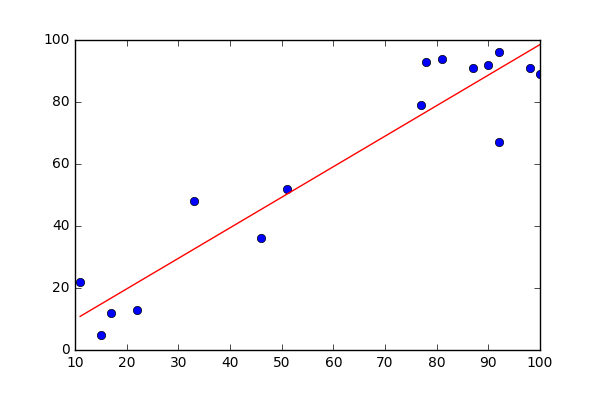
\includegraphics[width=10cm]{slike/fiz-kem-opt-model.png}
\caption{Ocene fizike in kemije na razsevnem diagramu.}
\label{f:fiz-kem-opt-model}
\end{center}
\end{figure}

\section{Multivariatna linearna regresija}

Približek ocene za kemijo izračunan iz ocene za fiziko je sicer čisto
v redu, a našo razredničarko in matematičarko mučijo ostale
ocene. Namreč, zgubila se je ocene za kemijo, vse ostale ocene pa
imamo. Ne samo za fiziko, ampak za slovenščino, matematiko, in
ostale. Bi lahko zgradili linearni model, ki bi upošteval tudi ostale
ocene? Torej, upošteval prav vse ostale atribute, ki so nam na
razpolago. In zgradil linearni model.

Ker imamo sedaj več atributov (variat) gre za multivariatno linearno
regresijo. Najprej nekaj sicer nam že dobro poznane notacije. Naj bo $x$ vektor atributnih vrednosti. Privzemimo, da so vsi atributi zvezni in da imamo $n$ različnih atributov, to je $x_1, x_2,\ldots x_n$. Označimo odvisno spremenljivko z $y$. Naš cilj je na podlagi učnih primerov, to je parov atributnih vektorjev in vrednosti odvisne spremenljivke $(x,y)$ zgraditi model:
%
\begin{equation}
h_\theta(x)=\theta_0 + \theta_1 x_1 + \ldots + \theta_n x_n
\end{equation}
%
Tokrat smo namesto parametrov $a$ in $b$ parametre modela označili s
črko $\theta$, ter parametrom modela dodali tudi indeks. Parameter
$\theta_0$ ustreza prejšnjemu parametru $b$, $\theta_1$ pa parametru
$a$. Da bo zapis bolj enostaven, določimo tudi $x_0$ ki naj vedno, to je, za vse primere, zavzame vrednost 1. Potem lahko zapišemo:
\begin{equation}
h_\theta(x) =\sum_{i=0}^n \theta_i x_i
\end{equation}
oziroma v vektorski obliki
\begin{equation}
h(x)=\theta^T x
\end{equation}

Parametre modela $\theta$ želimo izbrati tako, da bo napaka naše napovedi čim manjša. Napaka napovedi za $i$-ti primer, kjer je $\hat{y^{(i)}}$ napovedana vrednost, $y^{(i)}$ pa prava vrednost odvisne spremenljivke, je
%
\begin{equation}
\epsilon^{(i)}=\hat{y}^{(i)}-y^{(i)}=h_\theta(x^{(i)})-y^{(i)}
\end{equation}
%
Model smo tokrat označili s simbolom $h$, ker model predstavlja
hipotezo nad našimi podatki. Napake v negativno in pozitivno smer
obravnavamo enako, zato je kot prej tudi tu najbolje, da napako kar
kvadriramo. Zanimajo nas taki parametri, pri katerih je kvadrat napake
na učni množici minimalen, oziroma kjer se model čimbolj prilega učnim
podatkom:
\begin{equation}
\min_\theta\sum_{i=0}^m(h_\theta(x^{(i)})-y^{(i)})^2
\end{equation}

Na podlagi zgornjega kriterija zapišimo kriterijsko funkcijo. Kriterij
pomnožimo z $1\over 2$, da nam bo lažje kasneje pri izpeljavi odvodov, ter z $1/m$ da vrednost kriterijske funkcija ne bo odvisna od števila primerov:
%
\begin{equation}
J(\theta)={1\over 2m}\sum_{i=0}^m(h_\theta(x^{(i)})-y^{(i)})^2
\end{equation}
%
Naš cilj je sedaj poiskati take vrednosti parameterov, pri katerih bo
kriterijska funkcija $J(\theta)$ minimalna, oziroma take vrednosti,
pri katerem se bo glede na našo izbrano kriterijsko funkcijo naš
modelov čim bolje prilegal dani učni množici. 

\section{Metoda najhitrejšega spusta}

Iskanje optimalnih parametrov začnimo v neki točki, na primer kar v
$\theta=\vec{0}$. Potem spreminjamo $\theta$ tako, da se $J(theta)$
zmanšuje, to je, v nasprotni smeri parcialnega odvoda kriterijske
funkcije. Enako, kot smo počeli v prejšnjem poglavju z parametroma $a$
in $b$, le da tokrat ta korak zapišemo splošno za parameter $\theta_i$:
\begin{equation}
  \theta_i\leftarrow\theta_i-\alpha{\partial\over\partial\theta_i}J(\theta)
\end{equation}
%
Konstanto $\alpha$ imenujemo stopnja učenja, njena vrednost pa bo
narekovala, kako hitro bomo hiteli proti cilju. Če bo vrednost
$\alpha$ prevelika, je možno, da bo preleteli cilj in se odstrelili v
neskončnost. Če bo vrednost premajhna, bo konvergenca počasna.

Izpeljimo sedaj vrednost parcialnih odvodov oziroma vrednost
gradienta, ko parcialne odvode zložimo v vektor. Pri tem zaenkrat privzemimo, da bomo vrednosti parametra $\theta_i$ prilagodili enem samem primeru $(x,y)$:
%
\begin{eqnarray}
{\partial\over\partial\theta_i} J(\theta) & = & {\partial\over\partial\theta_i} {1\over 2m}(h_\theta(x)-y)^2 \\
& = & 2{1\over 2m}(h_\theta(x)-y){\partial\over\partial\theta_i}(h_\theta(x)-y) \\
& = & {1\over m}(h_\theta(x)-y){\partial\over\partial\theta_i}(\theta_0 x_0 + \ldots + \theta_i x_i + \ldots \theta_n x_n - y) \\
& = & {1\over m}(h_\theta(x)-y)x_i
\end{eqnarray}
%
Vsakokratni popravek parametra $\theta_i$ bo tako:
\begin{equation}
  \theta_i\leftarrow\theta_i-{\alpha\over m}(h_\theta(x)-y)x_i
\end{equation}
oziroma za vse primere:
\begin{equation}
  \theta_i\leftarrow\theta_i-{\alpha\over m}\sum_{j=1}^m(h_\theta(x^{(j)})-y^{(j)})x_i^{(j)}
\end{equation}

Pri linearni regresiji oziroma zgoraj opisanemu pristopu najmanjših kvadratov je $J(\theta)$ kvadratna funkcija z enim samim minimumom, zato se nam o tem, da bi se optimizacija zaustavila v nekem lokalnem minimumu ni potrebno bati. Lahko pa, kot smo že zapisali zgoraj, pri velikih vrednostih $\alpha$ minimum zgrešimo in se pričnemo vse bolj oddaljevati od njega. Pomaga seveda zmanjšanje $\alpha$ na vrednost, pri kateri je optimizacija stabilne in skonvergira k pravi vrednosti parametrov $\theta$.

\chapter{Regularizacija}

Pri vpeljavi linearne regresije v prejšnjem poglavju je bil cilj
gradnja modela, ki se čimbolj prilega učni množici. Pa je to res pravi
kriterij za določanje parametrov modela? Bo model, ki se najbolje
prileže učni množici res tisti, ki bo dobro napovedoval nove primere?
V tem poglavju pokažemo, da temu ni tako, nakažemo, kakšna bi bila
lahko rešitev problema in potem tudi povemo, da je ta žal odvisna od
parametra, ki ga moramo nekako oceniti iz podatkov. S tem smo sklenili
začarani krog (in morda nismo rešili prav dosti), a odprli skrinjico
problemov, ki je tipična za strojno učenje in znanost v podatkih.

\section{Polinomska regresija}

Na sliki~\ref{fig:poly-linear} so prikazani podatki, kjer linearni model očitno ni pravi in je odvisnost med atributom in razredom nelinearna. Linearni model z enim samim atributom, oziroma tako imenovani univariatni linearni model, očitno ne bo kos našemu problemu. 

\begin{figure}[htbp]
\begin{center}
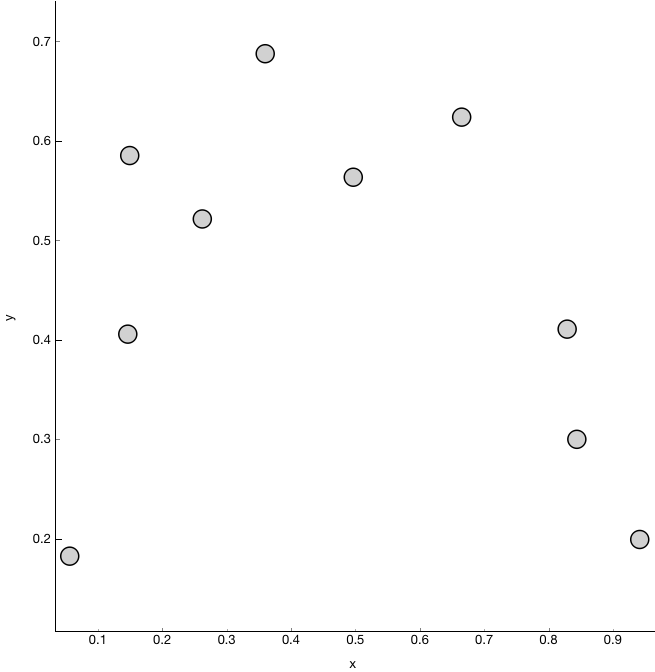
\includegraphics[width=0.45\textwidth]{slike/poly-linear.png}
\caption{Linearni model $y=\theta_0 + \theta_1 x$ se ne ujema dobro s podatki, saj je napaka velika, odvisnost med atributom $x$ in razredom $y$ pa očitno ni linearna.}
\label{fig:poly-linear}
\end{center}
\end{figure}

Model z eno samo spremenljivko zapišemo kot $y=\theta_0 + \theta_1 x$. Kaj pa, če podatke spremenimo tako, da število atributov povečamo. S stolpci, ki so potence našega osnovnega atributa. Torej, namesto, da vhodni podatki vsebujejo samo stolpec z atributom $x$, dodamo še stolpce potenc te spremenljivke, torej na primer stolpce z vrednostmi $x^2$ in $x^3$. Za trenutek uvedimo nova imena spremenljivk, oziroma nova imena atributov, in poimenujmo $a=x$, $b=x^2$ in $c=x^3$. S takimi spremenljivkami lahko zapišemo novi linearni model $y=\theta_0 + \theta_1 a + \theta_2 b + \theta_3 c$. S takimi modeli smo tudi že imeli opravka (v prejšnjem poglavju), zato nam niso novi. Še vedno gre za linearni model: torej model, kjer so $a$, $b$ in $c$ neke številke (vrednosti atributov za posamezni primer), ki so pomnožene s parametri modela $\theta_0\ldots\theta_3$, katerih vrednost iščemo.

Sedaj pa preoblikujmo naš model tako, da spet vstavimo potence atributa $x$. Tokrat se zavedajmo, da potenčni izrazi označujejo vrednosti atributov, torej nekih konstant iz naše tabele podatkov. Prav zato je model še vedno linearen:

$$ y=\theta_0 + \theta_1 x + \theta_2 x^2 + \theta_3 x^3 $$

Pravimo, da smo prostor atributov razširili s potenčnimi vrednostmi. Ker bomo nad tem prostorom gradili linearni regresijski model, temu postopku razširitve prostora atributov in gradnje linearnega modela pravimo polinomska regresija. In rezultat? Na sliki~\ref{fig:poly-linear-fit} je prikazan rezultat pri polinomski razširitvi stopnje 2 (uporabili smo atributa $x$ in $x^2$) ter stopnje štiri (uporaba atributov $x$, $x^2$, $x^3$ in $x^4$).

\begin{figure}[htbp]
\begin{center}
  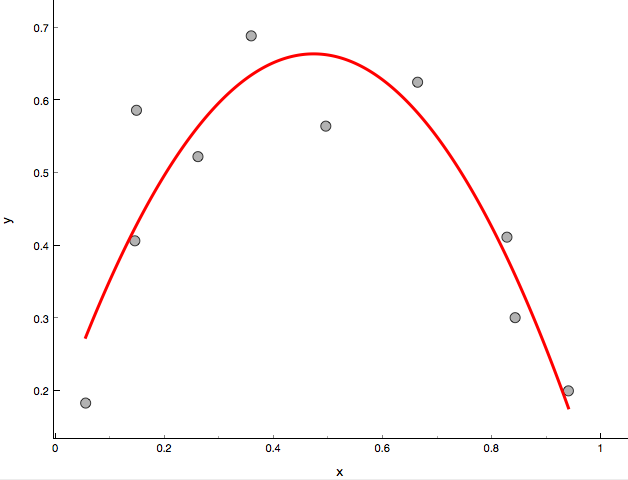
\includegraphics[width=0.45\textwidth]{slike/poly-reg-2.png}\hfill
  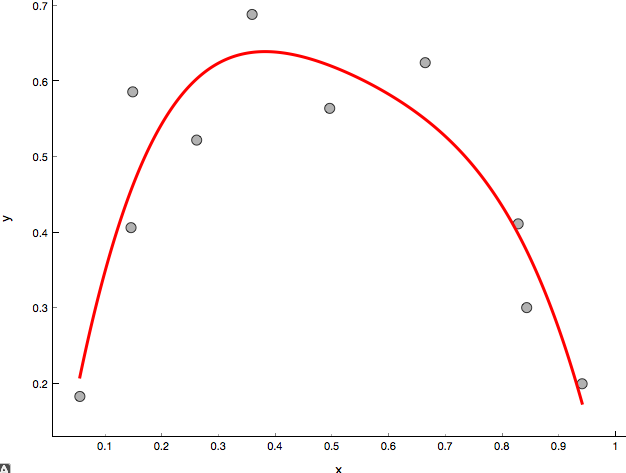
\includegraphics[width=0.45\textwidth]{slike/poly-reg-4.png}
\caption{Polinomska regresija druge in četrte stopnje.}
\label{fig:poly-linear-fit}
\end{center}
\end{figure}

Z dviganjem stopnje polinoma se naš model čedalje bolj prilega učnim podatkom, napovedna napaka oziroma naša kriterijska funkcija pa je čedalje manjša. S polinomsko razširitvijo sedmega reda smo dosegli skoraj popolno prileganje (slika~\ref{fig:poly-linear-fit7}). Vrednost naše kriterijske funkcije gre z dvigovanjem stopnje polinoma proti nič in je dejansko enaka nič takrat, ko je stopnja polinoma oziroma razširitve atributnega prostora enaka $m-1$, kjer je $m$ število primerov.

\begin{figure}[htbp]
\begin{center}
  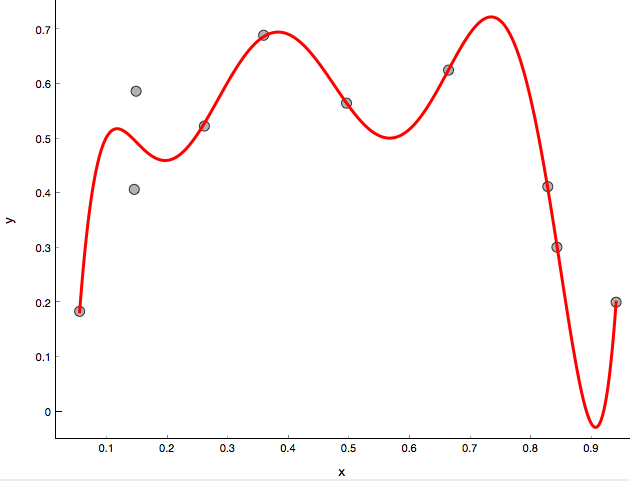
\includegraphics[width=0.45\textwidth]{slike/poly-reg-7.png}
  \hfill
  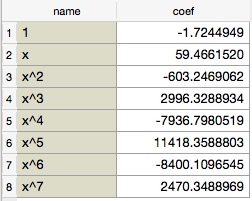
\includegraphics[width=0.45\textwidth]{slike/poly-reg-7-coeff.png}
\caption{Polinomska regresija sedme stopnje in koeficienti modela.}
\label{fig:poly-linear-fit7}
\end{center}
\end{figure}

Navidezno smo problem iskanja modela, ki bi minimiziral kriterijsko fukcijo, z uvedbo polinomske regresije rešili. Pa smo res? Spomnimo se, da je naš cilj gradnje modelov napovedovanje, torej ne samo modeliranje na osnovi učne množice, ampak uporaba modela za napovedovanje primerov, ki jih pri učenju nismo videli in ki so novi. Uporabo polinomske regresije moramo zato preskusiti na tovrstnih primerih, ki jim pravimo tudi testna množica. Pred tem pa se moramo dogovoriti, kako bomo merili uspešnost modela oziroma njegovo napovedno točnost.

\section{Napovedna točnost}

Imejmo testno množico $\cal{T}$ s $k$ primeri, $k=|\cal{T}|$, za katere poznamo njihov atributni opis $x^{(i)}$ in vemo njihov pravi razred $y^{(i)}$. Oceniti želimo napovedno točnost regresijskega modela, ki za $i$-ti primer napove oziroma oceni vrednost njegovega razreda kot $\hat{y}^{(i)}$.

Pri prvi meri za napovedno točnost, ki jo bomo tu uvedli, sledimo dosedanji logiki, da nas predznak napake ne zanima (torej kvadriramo) in da bi radi izračunali povprečno vrednost take, kvadrirane napake. Ker bi želeli, da se napaka izrazi v istih enotah kot vrednosti razreda v učni množici, povprečno kvadrirano napako na koncu še korenimo. Dobimo koren povprečne kvadrirane napake \angl{Root Mean Squared Error}):

$$ {\rm RMSE}(\cal{T})=\sqrt{\sum_{i=1}^k{y^{(i)}-\hat{y}^{(i)}}\over k} $$

Mera RMSE je sicer čisto v redu, a je njena vrednost odvisna od domene odvisne spremenljivke. Na primer, če je ${\rm RMSE}=42.0$ s tem pravzaprav nismo povedali ničesar, saj ne poznamo razpon odvisne spremenljvike. Če smo s tem ocenili težo tovornjakov v tonah, je napaka ogromna, če pa smo njegovo težo ocenjevali v kilogramih, je skoraj zanemarljiva. Bolje bi bilo imeti oceno napake, kjer je ta neodvisna od domene odvisne spremenljivke. Recimo, nekaj, čemur statistiki pravijo delež razložene variance:

$$ R^2({\cal T})=1-{\sum_k (y^{(i)}-\hat{y}^{(i)})^2
  \over \sum_k(y^{(i)}-\bar{y})^2} $$

V imenovalcu ulomka je vsota kvadratov napak, ki bi jo naredili, če bi model napovedoval s povprečno vrednostjo odvisne spremenljivke učne množice. To bi bil prav slab model in pričakujemo, da bo njegova napaka večja, ali pa morda veliko večja od te, ki bi jo naredil boljši model in katerega kvadrat napake izračunamo v števcu ulomka. Za zelo dober model gre člen z ulomkom proti vrednosti 0, ocena $R^2$ pa zato proti vrednosti 1. Slabši modeli pa bodo imeli napako le malo manjšo od napake napovedi s povprečno vrednostjo.

Ocena $R^2$ bo takrat šla proti 0. Delež razložene variance ima zato pričakovano vrednost med 0 in 1. Opozorimo le, da čeprav vemo, da bodo visoke vrednosti $R^2$, torej take blizu 1.0 zaželene, so lahko uporabni tudi modeli z vrednosti $R^2$ blizu nič. Na primer, z modelom, ki ima na testni množici pri napovedi tečaja neke valute $R^2=0.1$ bi obogateli, model z isto točnostjo za napoved jutrišnje povprečne temperature pa bi lahko vrgli v koš.

\section{Ocenjevanje napovedne točnosti}

Naredimo eksperiment: učno množico, ki jo prikazuje slika~\ref{fig:poly-reg-many}, naključno razdelimo na polovico, kjer uporabimo polovico naključno izbranih primerov za učenje linearnega modela, na drugi polovici modela pa testiramo napovedno uspešnost. Za ocenjevanje točnosti smo uporabili $R^2$, in to merili na učni in testni množici.

\begin{figure}[htbp]
\begin{center}
  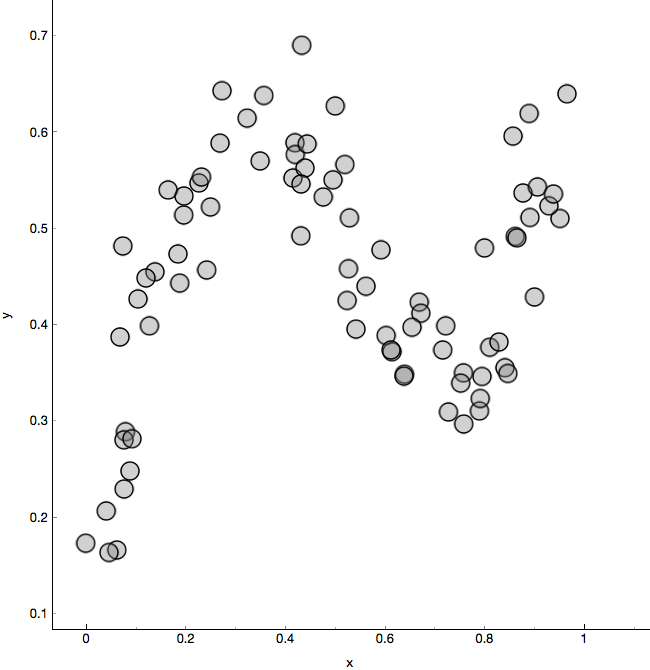
\includegraphics[width=0.45\textwidth]{slike/poly-reg-many.png}
\caption{Množica vseh primerov, ki jih naključno porazdelimo med učno in tesno množico za ocenjevanje gradnjo in ocenjevanje kvalitete modela polinomske regresije.}
\label{fig:poly-reg-many}
\end{center}
\end{figure}

Rezultate kaže tabela~\ref{tab:poly-reg-many-res}. S stopnjo polinomske razširitve atributnega prostora napovedna točnost modela na učni množici monotono narašča. Na množici testnih primerov pa je slika drugačna: s kompleksnostjo modela napovedna točnost nekaj časa narašča, potem pa strmo pade. Pravimo, da se je model preveč prilegel učni množici, postal zato prekompleksen in ni zajel glavnih vzorcev, ki so prisotni tudi v novih primerih.

\begin{table}
  \caption{Delež razložene variance na učni in testni množici (podatki s slike~\ref{fig:poly-reg-many}) za polinomsko regresijo stopnje $k$.}
  \begin{center}
  \begin{tabular}{ccc}
    \hline
    k & učna & testna \\
    \hline
    0 & 0.000 & 0.002 \\
    1 & 0.031 & 0.037 \\
    2 & 0.161 & 0.151 \\
    3 & 0.806 & 0.688 \\
    4 & 0.822 & 0.687 \\
    5 & 0.832 & 0.715 \\
    6 & 0.841 & 0.716 \\
    7 & 0.841 & 0.714 \\
    8 & 0.857 & 0.365 \\
    9 & 0.863 & 0.118 \\
    \hline
  \end{tabular}
  \end{center}
  \label{tab:poly-reg-many-res}
\end{table}

\section{Regularizacija linearne regresije}

Ko višamo stopnjo polinomske razširitve atributnega prostora smo opazili (slika~\ref{fig:poly-linear-fit7}), da parametri modela podivjajo, oziroma postane njihova vrednost zelo visoka. Kar ni nič čudnega, saj se model zelo prilagodi učnim podatkom, funkcija odvisnosti med $x$ in $y$ je zelo razgibana, njeni odvodi pa zelo visoki. Prileganje učni množici se torej izrazi v absolutno velikih vrednostih parametrov modela (absolutno zato, ker so te vrednosti lahko visoke a negativne ali visoke in pozitivne). Želeli bi si manj ``divje'' modele, torej take, kjer bi bili parametri modela po absolutni meri manjši. To željo enostavno izrazimo kot dodatek h kriterijiski funkciji za linearno regresijo:

\begin{equation}
J = {1\over 2m}\sum_{i=1}^m (f(y^{(i)})-y^{(i)})^2 + \eta\sum_{j=1}^n \theta_j^2
\end{equation}

Prvi člen v zgornji enačbi je cenovna funkcija za linearno regresijo, kjer želimo, da se model čimbolj prilega učni množici. Drugi člen pa pravi, da naj bo kvadratna vrednost parametrov takega modela čim manjša. Uporabili smo kvadratno vrednost parametrov, saj nam je vseeno, ali je njihova vrednost pozitivna ali negativna. Pravimo, da smo cenovno funkcijo regularizirali, stopnjo regularizacije pa uravnavamo z vrednostjo $\eta$, katere tipične vrednosti so nizke, recimo 0.1 ali pa 0.01 ali pa celo 0.0001.

Za učenje modela linearne regresije, torej, za določanje vrednosti parametrov $\theta_i$ modela iz podatkov rabimo še izračunati gradient. Izračun je enostaven, saj je enak, kot pri neregularizirani linearni regresiji plus odvod člena za regularizacijo (spodnja enačba velja za $i=1\ldots n$, za $i=0$ pa ostane odvod enak kot prej):

\begin{equation}
{\partial\over\partial\theta_i} J(\theta) = {1\over m}(h_\theta(x)-y)x_i + \eta\theta_i
\end{equation}

Ostane le še preskus: ali se, tudi z regularizacijo, lahko preveč prilagodimo manjšemu naboru podatkov v učni množici. Seveda je vse odvisno od stopnje regularizacije $\eta$, a v splošnem (pri primerni vrednosti parametra $\eta$) je odgovor ne. Regularizacija nam pomaga pri preprečevanju prevelikega prileganja. Naj sliki~\ref{fig:poly-reg-compare} je tako primer podatkov in polinomske regresije brez regularizacije in z regularizacijo.

\begin{figure}[htbp]
\begin{center}
  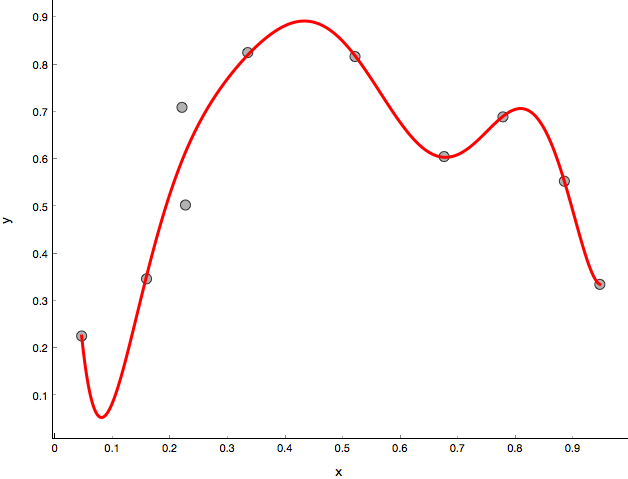
\includegraphics[width=0.45\textwidth]{slike/poly-reg-no.png}
  \hfill
  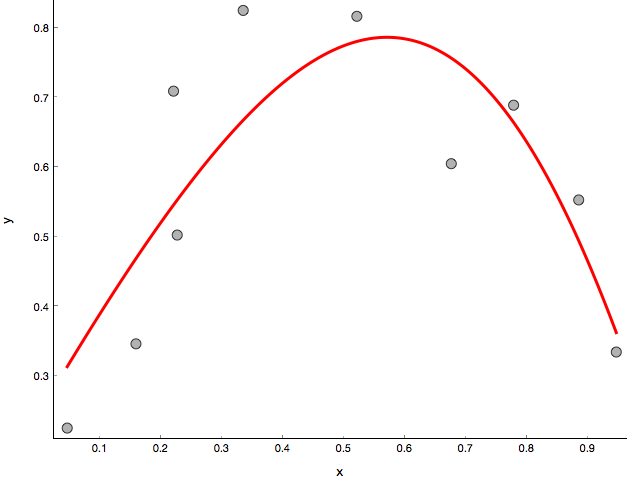
\includegraphics[width=0.45\textwidth]{slike/poly-reg-yes.png}
\caption{Model polinomske regresije stopnje osem brez (levo) in z regularizacijo ($\eta=0.01$, desno).}
\label{fig:poly-reg-compare}
\end{center}
\end{figure}

\chapter{Logistična regresija}

Se bo osnovnošolec Vinko uvrstil v drugi krog tekmovanja iz kemije? Se bo po srednji šoli vpisal na Kemijsko fakulteto? Ga bo zaposlilo podjetje, ki se ukvarja z biofarmacijo? Bo njegov košarkaški klub Olimpija premagal Crveno zvezdo to soboto? Se bo poročil s sosedovo Niko? Bo njegova ideja o tekočini, ki vsakih 35 minut spremeni barvo, uspela na Kickstarterju?

Morda smo s kakšnim od zgornjih vprašanj zašli, a na vsaj eno od naštetih vemo, da je nanj možno dovolj dobro odgovoriti. So pa to vprašanja, ki niso regresijska, oziroma je napoved kategorična tipa ``bo'' ali ``ne bo''. Še bolj natančno: za vsako od zgornjih vprašanj bi pravzaprav radi ocenili verjetnost, ali se bo nek dogodek zgodil. Recimo, zanima nas, s kakšno verjetnostjo se bo Vino poročil z Niko. In pa, s kakšno verjetnostjo se bo njegov kicksterski projekt uspel.

Seveda bomo tudi tokrat napovedne modele, tokrat klasifikacijske, gradili iz podatkov. Za silo bi take podatke in s tem problem spremenili v regresijskega tako, da bi odgovore označili z vrednostjo 0 (dogodek se ni zgodil) ali 1 (dogodek se je zgodil), potem pa to vrednost obravnavali kot zvezno vrednost odvisne spremenljivke oziroma razreda $y$. Primer take obravnave nam kaže tabela~\ref{f:temperatura} s podatki o obiskovalci ordinacije, ki jim je zdravnik zmeril telesno temperaturo in potem (na podlagi dodatnih preiskav, seveda, ki pa jih tu ne podajamo) določil zdravstveno stanje. Naš cilj je zgraditi model, ki zdravstveno stanje oceni (samo) na podlagi telesne temperature.

\begin{table}[htbp]
\caption{Telesna temperatura in stanje pregledovanca, ki smo ga zapisali v numerični obliki kot razred $y$.}
\label{f:temperatura}
\begin{center}
\begin{tabular}{ccc}
\toprule
temperatura & stanje & $y$ \\
\midrule
36,5 & zdrav & 0 \\
36,6 & zdrav & 0 \\
36,8 & zdrav & 0 \\
36,9 & bolan & 1 \\
37,0 & zdrav & 0 \\
37,2 & bolan & 1 \\
37,5 & bolan & 1 \\
37,6 & bolan & 1 \\
39,5 & bolan & 1 \\
\bottomrule
\end{tabular}
\end{center}
\end{table}

Podatke predstavimo grafično (slika~\ref{f:class-linreg}) in si potem drznemo vpeti linearno funkcijo $y=h(x)$. Najprej opazimo, da je zaloga vrednosti funkcije $h(x)$ neprimerna, saj gre ta od $-\infty$ do $\infty$. Na intervalu telesnih temperatur okoli točke $37^{\circ}$ ima funkcija sicer vrednost med 0 in 1. Pojavi pa se vprašanje, kako vrednost te linearne funkcije sploh interpretirati, oziroma kako jo pretvoriti v verjetnost. Spomnimo se, da vsaka verjetnostna funkcija vrača vrednosti med 0 in 1, naša linearna funkcija pa je omejena na ta interval samo v določenem območju vrednosti vhodnega atributa. Dodaten problem je še z osamelci, oziroma obiskovalci s skrajnimi vrednostnimi atributov. Če bi podatkom dodali še en primer bolnika z zelo visoko temperaturo, bi se naša funkcija precej spremenila in pomaknila nagnila v desno. Potrebujemo nek predpis, ki bi vrednosti take funkcije pretvoril v verjetnosti in jih morda blizu $y=0$ in $y=1$ malce zmehčal.

\begin{figure}[htbp]
\begin{center}
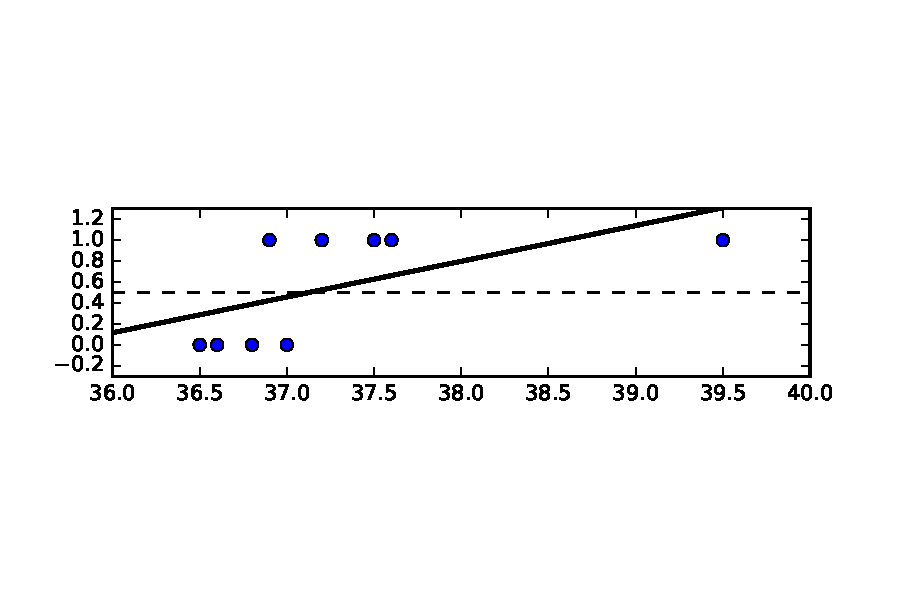
\includegraphics[width=10cm]{slike/class-linreg.pdf}
\caption{Poskus klasifikacije z linearno regresijo.}
\label{f:class-linreg}
\end{center}
\end{figure}

\section{Logistična funkcija}

Funkcija, ki jo bomo uporabili in ki neko realno število pretvori v število na intervalu [-1, 1], je logistična funkcija (slika~\ref{f:logistic-function}):
\begin{equation}
  g(z) = {1\over 1+e^{-z}}
\end{equation}

\begin{figure}[htbp]
\begin{center}
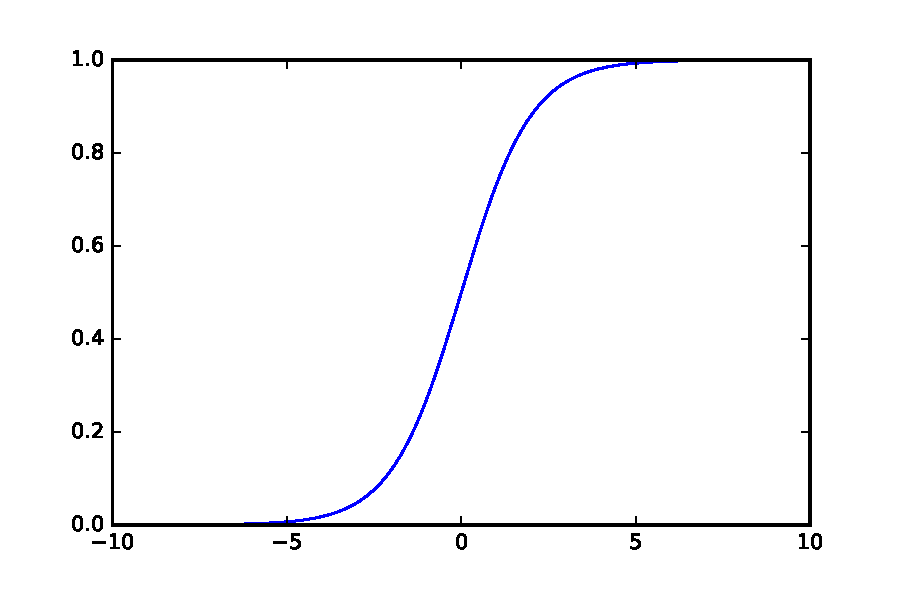
\includegraphics[width=10cm]{slike/logistic.pdf}
\caption{Logistična funkcija.}
\label{f:logistic-function}
\end{center}
\end{figure}

Logistična funkcija je zvezna, monotona, z $z\to -\infty$ konvergira proti 0 in z $z\to\infty$ proti 1. Je odvedljiva pri vseh vrednosti njenega parametra. Njen odvod je:
\begin{eqnarray}
  \frac{dg(z)}{dz} & = & \frac{d}{dz} \frac{1}{1+e^{-z}} \nonumber \\
  & = & \frac{1}{(1+e^{-z})^2} e^{-z} \nonumber \\
  & = & \frac{1}{1+e^{-z}}\frac{e^{-z}}{1+e^{-z}} \nonumber \\
  & = & \frac{1}{1+e^{-z}}\frac{1+e^{-z}-1}{1+e^{-z}} \nonumber \\
  & = & \frac{1}{1+e^{-z}}\big(1-\frac{1}{1+e^{-z}}\big) \nonumber \\
  & = & g(z)[1-g(z)]
\end{eqnarray}

\section{Logistična regresija}

Zapišimo sedaj naš klasifikacijski model. V osnovi bo to linearni model, torej utežena vsota vrednosti atributov. A tokrat jo bomo, zato, da bo vrednost modela izražala pripadnost (verjetnost) ciljnemu razredu, transformirali z logistično funkcijo:
\begin{eqnarray}
  h_\Theta(x) & = & g(\theta_0+\theta_1 x_1+\theta_2 x_2+\ldots\theta_n x_n)
  \nonumber \\
  & = & g(\Theta^T x) \nonumber \\
  & = & \frac{1}{1+e^{-\Theta^T x}}
  \label{eq:logreg}
\end{eqnarray}

Model zaradi uporabe logistične funkcije imenujemo {\em logistična regresija}.

\section{Računanje verjetnosti razreda}

V nadaljevanju bomo torej logistično funkcijo uporabili tako, da nam bo naš model $h_{\Theta}(0)$, ki je v osnovi linearni model, vračal vrednosti med 0 in 1. Še naprej bomo predpostavljali, da je naša razredna spremenljivka dvovrednostna, a privzeli, da je njena ciljna vrednost razred z oznako $y=1$ in da zanj model $h_{\Theta}(x)$ vrača verjetnost tega razreda. K oznaki modela smo namenoma pripisali oznako za vektor parametrov $\Theta$ in na ta način poudarili, da ti parametri tudi polno opredelijo naš model. Zapišemo torej lahko:
\begin{eqnarray}
  P(y=1|x;\Theta) & = & h_\Theta(x) \\
  P(y=0|x;\Theta) & = & 1-h_\Theta(x)
\end{eqnarray}
Izraz za $P(y=1|x;\Theta)$ nam torej podaja verjetnost, da je razred primera, ki je opisan z vektorjem atributnih vrednosti $x$, enak 1. Oziroma podaja verjetnost, da neodvisna spremenljivka zavzame vrednost 1 pri opisu primera $x$ in parametrizaciji modela s parametri $\Theta$. En sam izraz, ki združi zgornji enačbi v eno in ki podaja verjetnostno porazdelitev za spremenljivko $y$ je:
\begin{equation}
  p(y|x;\Theta) = (h_\Theta(x))^y(1-h_\Theta(x))^{1-y}
\label{eq:log-prob}
\end{equation}
Pravilnost zgornjega izraza preveri tako, da za vrednost spremenljivke $y$ vstaviš enkrat $y=1$ in drugič $y=0$.

\section{Verjetje}

Izraz za $p(y|x;\Theta)$ v enačbi~\ref{eq:log-prob} torej podaja verjetnost za določeno vrednost neodvisne spremenljivke in določen vektor atributnih vrednosti pri modelu, ki je podan z $\Theta$. Sedaj pa si predstavljamo, da vrednosti elementov vektorja $\Theta$ spreminjamo. Prav gotovo se bo na ta način tudi spreminjala verjetnost za dani razred pri izbranem primeru; enkrat bo ta verjetnost višja, drugič nižja.

Zamrznimo sedaj parametre modela $\Theta$ in izračunajmo verjetnosti $L(\Theta)$ pravih razredov $\vec{y}$ za primere v učni množici, ki jo opišemo z matriko atributnih vrednosti $X$. Predpostavljamo, da so primeri iz učne množice neodvisni in da zato verjetnost za vrednosti spremenljivke $y$ za celotno učno množico lahko zapišemo kot produkt verjetnosti za vrednost $y$ za posamezne primere:
\begin{eqnarray}
  L(\Theta) & = & p(\vec{y}|X;\Theta) \nonumber\\
  & = & \prod_{i=1}^m p(y^{(i)}|x^{(i)};\Theta) \nonumber\\
  & = & \prod_{i=1}^m h_\Theta(x^{(i)})^{y^{(i)}}(1-h_\Theta(x^{(i)}))^{1-y^{(i)}}
\end{eqnarray}

Kot smo označili v zgornji funkciji $L$, je ta verjetnost odvisna od parametrov modela $\Theta$. Kakšen model bi želeli imeti? Tak, pri katerem je verjetnost $L(\Theta)$ največja. Torej tak model, kjer bo verjetnost, da bo model napovedal take vrednosti razredov, kot so v učni množici, največja. $L(\Theta)$ igra vlogo kriterijske funkcije, ki pa jo tokrat maksimiziramo.

Funkcijo $L$ imenujemo {\em verjetje}. Iščemo torej parametre $\Theta$, kjer je njena vrednost največja. Tudi tokrat bomo tako vrednost parametrov iskali z gradientnimi pristopi, za te pa sedaj že vemo, da moramo znati izračunati odvode po posameznih parametrih, oziroma, da moramo znati izračunati gradient kriterijske funkcije. Ker je odvajanje funkcij z mnogo produkti, torej funkcij, kot je naša $L(\Theta)$, precej mučno, se vprašajmo, ali obstaja kakšna preslikava funkcije $L$, za katero bi bilo lažje izračunati odvod in pri kateri bi vrednosti $\Theta$, ki to funkcijo maksimizirajo prav tako maksimizirajo tudi funkcijo $L(\Theta)$. Taka preslikava je logaritemska funkcija, ki je na intervalu od 0 do $\infty$ monotona in bo torej vektor $\Theta$, ki maksimizira $\log(L(\Theta))$ torej tak, da maksimizira tudi $L(\Theta)$. Logaritem $L(\Theta)$ označimo kot $l(\Theta)$ in ga izračunamo kot:
\begin{eqnarray}
  l(\Theta) & = & \log L(\Theta) \nonumber\\
  & = & \sum_{i=1}^m\big[y^{(i)}\log h_\Theta(x^{(i)})+(1-y^{(i)})\log (1-h_\Theta(x^{(i)})) \big]
\end{eqnarray}

Namesto kriterijske funkcije $L(\Theta)$ bomo torej uporabili funkcijo $l(\Theta)$, ki ji pravimo tudi {\em logaritem verjetja} (angl. {\em log likelihood}).

\section{Gradient logaritma verjetja}

Iščemo torej tak $\Theta$, ki maksimizira logaritem verjetja $l(\Theta)$. Ker bomo uporabili gradientno metodo in ker je $\Theta$ vektor $[\theta_0 \theta_1 \ldots \theta_n]$, moramo izračunati parcialne odvode naše kriterijske funkcije:
\begin{eqnarray}
  \frac{\partial}{\partial\theta_j}l(\Theta)
  & = & \sum_{i=1}^m \frac{\partial}{\partial\theta_j} \big[y^{(i)}\log h_\Theta(x^{(i)})+(1-y^{(i)})\log (1-h_\Theta(x^{(i)})) \big] \nonumber \\
  & = & \sum_{i=1}^m \big[y^{(i)}\frac{1}{g(\Theta^T x^{(i)})}-(1-y^{(i)})\frac{1}{1-g(\Theta^T x^{(i)})} \big]\frac{\partial}{\partial\theta_j}g(\Theta^T x^{(i)}) \nonumber\\
  & = & \sum_{i=1}^m \big[\frac{y^{(i)}}{g(\Theta^T x^{(i)})}-\frac{(1-y^{(i)})}{1-g(\Theta^T x^{(i)})} \big]g(\Theta^T x^{(i)})(1-g(\Theta^T x^{(i)}))
  \frac{\partial}{\partial\theta_j}\Theta^T x^{(i)}\nonumber\\
  & = & \sum_{i=1}^m \big[\frac{y^{(i)} - g(\Theta^T x^{(i)})} {g(\Theta^T x^{(i)})(1-g(\Theta^T x^{(i)}))} \big]g(\Theta^T x^{(i)})(1-g(\Theta^T x^{(i)})) x_j^{(i)}\nonumber\\
  & = & \sum_{i=1}^m (y^{(i)}-g(\Theta^T x^{(i)}))x_j^{(i)}\nonumber\\
  & = & \sum_{i=1}^m (y^{(i)}-h_\Theta(x^{(i)}))x_j^{(i)}\nonumber
  \label{eq:logreg-grad}
\end{eqnarray}
Zelo enostavno! Smo tak rezultat oziroma tako enačbo videli že kje prej? Seveda! Pri linearni regresiji. Parcialni odvodi so identična tem za linearno regresijo. Seveda z majhno razliko. Tokrat naša funkcija $h_\Theta$ uporablja logistično funkcijo (en.~\ref{eq:logreg}), pri linearni regresiji pa je bila $h_\Theta$ samo utežena vsota atributnih vrednosti.

\section{Optimizacija parametrov modela}

Postopek iskanja parametrov modela je identičen temu pri linearni regresiji. Seveda, z majhno razliko, da je tokratni model $h_\Theta(x)$ model logistične regresije. Vseeno zapišimo korak za osveževanje vrednosti parametra $\theta_j$:
\begin{equation}
  \theta_j\leftarrow\theta_j+\alpha\sum_{i=1}^{m}\big(y^{(i)}-h_\Theta(x^{(i)})\big) x_j^{(i)}
\end{equation}

Tudi tokrat je $\alpha$ stopnja učenja, katerega vrednost je pri normaliziranih podatkih tipično majhna (npr. $0.001$).

Tukaj velja opozorilo. Pristop z gradientnim sestopom je počasen in je, že za srednje velike podatke, potrebno izvesti mnogo iteracij popravljanja vrednosti parametrov $\Theta$. Namesto te tehnike tipično uporabljamo optimizacijske tehnike, ki imajo hitrejšo konvergenco. Ena od teh je postopek L-BFGS, ki pa ga tipično uporabimo iz za to dostopne knjižnice. Na vhodu postopek L-BFGS potrebuje cenovno funkcijo (torej, $l(\Theta)$) in pa njen gradient, ki smo ga izračunali zgoraj (en.~\ref{eq:logreg-grad}).

\chapter{Klasifikacijska drevesa in gozdovi}

Drevesa in gozdovi za klasifikacijo so zelo podobna tem za regresijo. Edina večja razlika je le v načinu ocenjevanja pomembnosti atributov. V tem poglavju se zato najprej seznanimo s temi metodami in jih potem uporabimo pri gradnji dreves in gozdov.

\section{Ocenjevanje pomembnosti atributov\label{c-attribute-scoring}}

Pri prav vseh praktičnih problemih uvrščanja v skupine nas zelo zanimajo atributi, ki so kar najbolj povezani z znanimi uvrstitvami primerov oziroma, kot bi temu rekli v strojnem učenju, z razredi primerov. Razkritje takih atributov nam lahko dosti pove o problemu, ki ga raziskujemo, odkrije, katere lastnosti opazovanih objektov moramo spremljati še v prihodnje oziroma so tiste, ki igrajo pomembno vlogo pri računalniški podpori odločanja. Velika večina tehnik ocenjevanj pomembnosti atributov obravnava en sam atribut ločeno od ostalih, to je, zanemari kakršnekoli medsebojne povezanosti atributov. Peščica tehnik, med katerimi bomo tu omenili eno samo, najbolj znano, pa zna razkriti pomembnost atributa tudi z ozirom na kontekst, to je, skladno z vrednostmi ostalih atributov.

Začnimo pri tehnikah, ki atribute obravnavajo vsakega zase in kontekst ostalih atributov zanemarijo. Za začetek poglejmo množico trikotnikov in kvadratov s slike~\ref{f-squares-triangles}. Želeli bi oceniti, kako dobro lahko na podlagi barve lika napovemo njegovo obliko. 

\begin{figure}[htbp]
\begin{center}
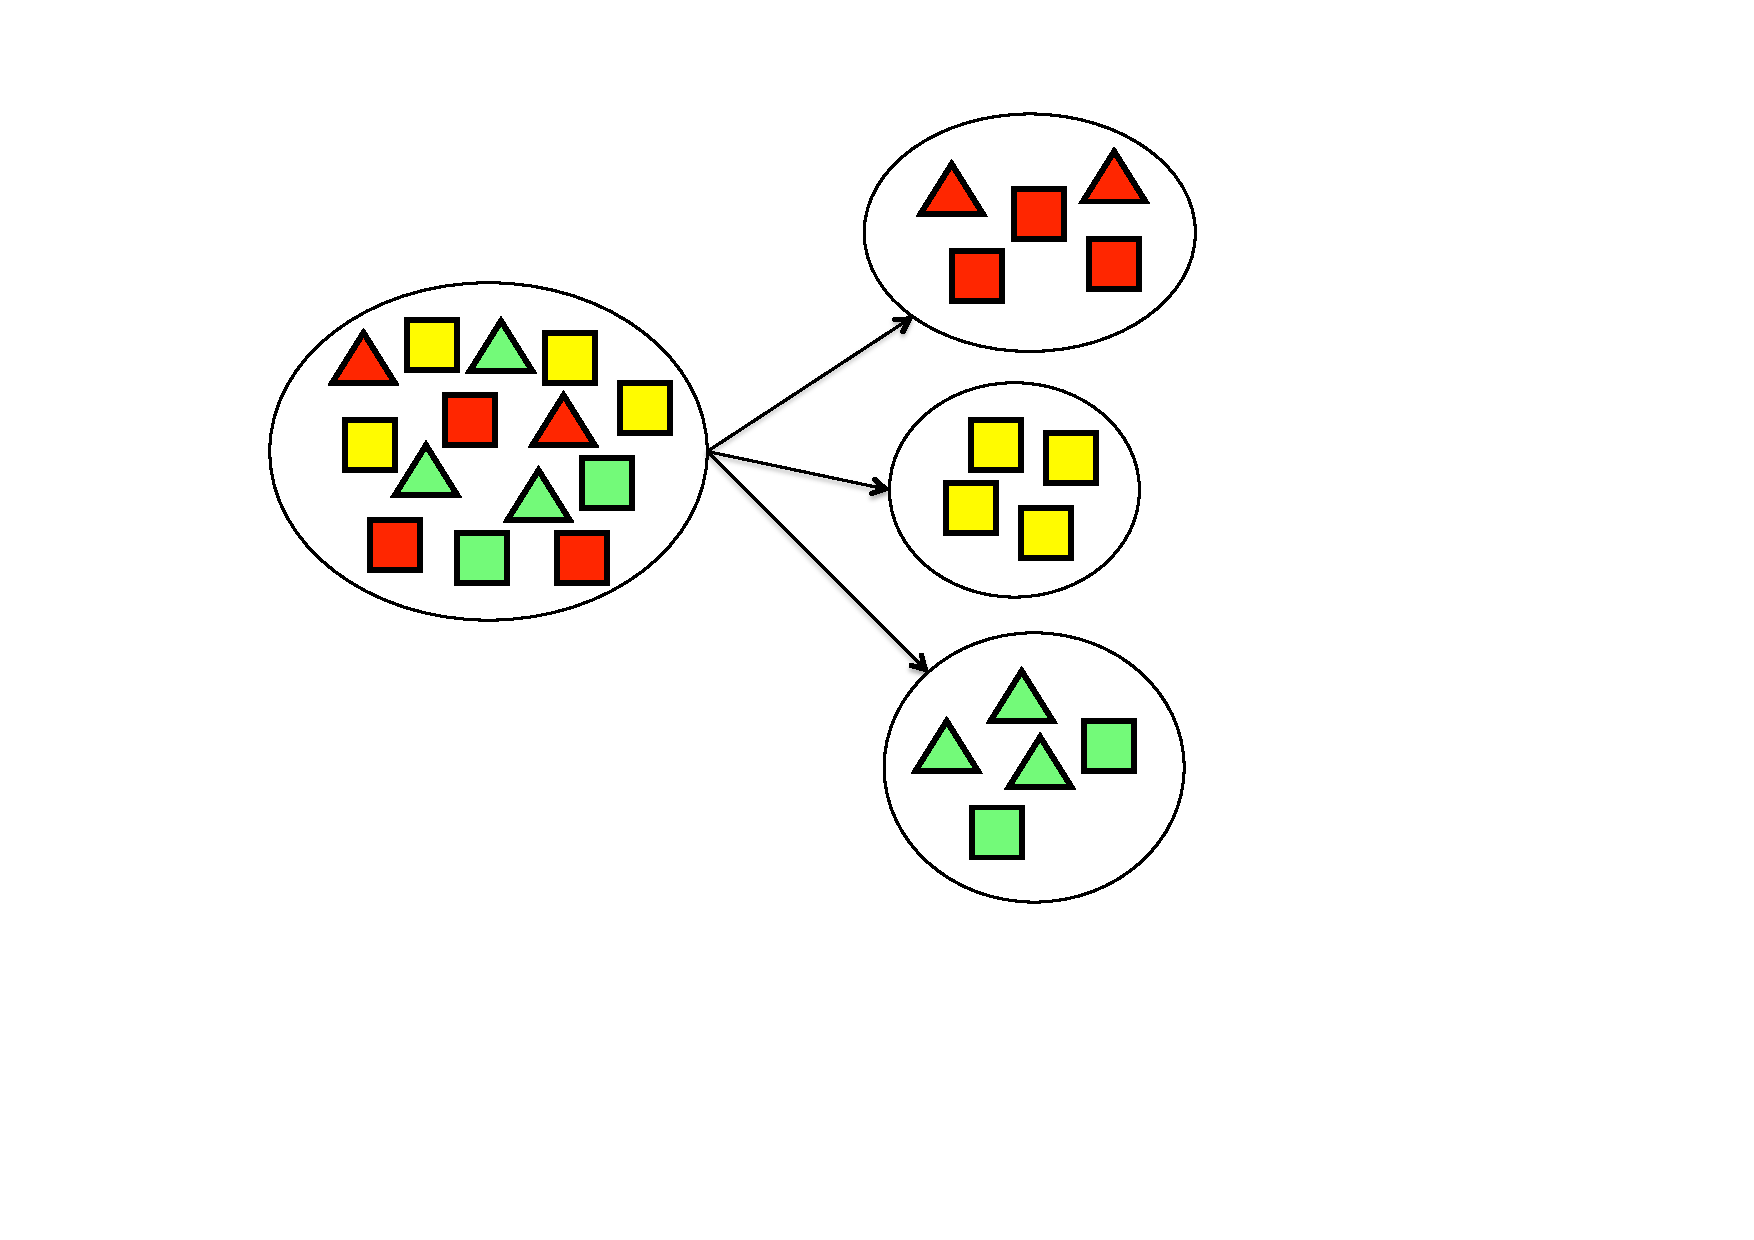
\includegraphics[width=7cm]{slike/squares-triangles.pdf}
\caption{Množica različno obarvanih kvadratov in trikotnikov (levo) in ista množica razdeljena na tri podmnožice glede na barvo likov. Vseh likov skupaj je $N=14$.}
\label{f-squares-triangles}
\end{center}
\end{figure}

\subsection{Informacijski prispevek}

Če bi bila povezanost med barvami in oblikami likov popolna, bi bile v posameznih podmnožicah na desni strani slike~\ref{f-squares-triangles} vsi liki enakih oblik. Pa niso. Pravimo, da množice niso čiste. Podmnožica rumenih likov je čista, čistočo ostalih pa bi radi zmerili. Obliko likov, naš razred, obravnavajmo kot naključno spremenljivko $C$, njene vrednosti pa označimo z $c_i$. Naša spremenljivka ima dve različni vrednosti, ``trikotnik'' in ``kvadrat''. Ocenimo še verjetnosti, da med liki iz naše celotne množice likov ($N=14$) izberemo, na primer, trikotnik. Za oceno uporabimo kar relativno frekvenco:
%
$$ P_{\triangle}={N_{\triangle} \over N} = 5/14 = 0.357 $$
%
Podobno izračunamo, da je $P_{\Box}= 0.643$. Nečistočo naše množice likov lahko ocenimo z entropijo $H$ diskretne naključne spremenljive $C$, ki je, izmerjena v bitih:
%
$$ H(C) = \sum_{i=1}^n {p(c_i)\,I(c_i)} = -\sum_{i=1}^n {p(c_i) \log_2 p(c_i)} $$
%
oziroma za naš primer:
$$ H(C) = - 0.357 \times log_2 0.357 - 0.643 \times log_2 0.643 = 0.940 $$

Ravno tako, kot za osnovno množico, lahko ocenimo nečistočo podmnožic, ki jih dobimo, ko smo like razdelili glede na njihovo barvo. Tako dobimo:
%
$$ H(C|{\rm color=red}) = -\plogp{3}{5}-\plogp{2}{5}=0.971 $$
$$ H(C|{\rm color=yellow}) = -\plogp{4}{4}-\plogp{0}{4}=0.0 $$
$$ H(C|{\rm color=green}) = -\plogp{2}{5}-\plogp{3}{5}=0.971 $$

Oceniti moramo še verjetnost, da lik pripada eni od podmnožic. Z drugimi besedami, kakšna je verjetnost, da bo naključno izbran lik iz naše osnovne množice na primer rdeč. Enostavno, 
%
$$ P_{\rm red}={N_{\rm red}\over N} = {5\over 14}=0.357$$
%
Podobno ocenimo še $P_{\rm yellow}=0.286$ in $P_{\rm green}=0.357$. Pričakovana nečistoča podmnožic, ko našo množico likov razdelimo skladno z njihovo barvno, ocenimo kot vsoto nečistoč podmnožic, ki jo utežimo z verjetnostjo, da bo lik pripadal določeni množici. Dobljeni uteženi vsoti pravimo residualna entropija:
%
$$ H_{res}=H(C|X)=\sum_{_i} p(x_i) H(C|x_i)  $$
%
in za naš primer znaša:
$$ H_{res} = 0.357 \times 0.971 + 0.0 \times 0.971 + 0.357 \times 0.971 = 0.694 $$

Pričakovana entropija, ko smo like razdelili po barvi, je torej manjša od entropije osnovne množico. Njuni razliki pravimo informacijski prispevek \angl{information gain} in z njim ocenimo, koliko informacije nam prispeva poznavanje vrednosti posameznega atributa:
$$ {\rm IG}(X) = H(C) - H(C|X) = 0.940 - 0.694 = 0.246 $$

\subsection{Relativni informacijski prispevek}

Pri atributih, ki imajo veliko zalogo vrednosti, se nam prav lahko zgodi, da nam ti primere iz osnovne množice razdelijo v zelo majhne podmnožice, morda celo take s po enim samim elementom. Entropija oziroma nečistoča slednjih je nič, a takih podmnožic si vsekakor ne želimo. Pravzaprav lahko informacijski prispevek favorizira atribute z veliko zalogo vrednosti. To ``prednost'' lahko uravnotežimo s tem, da se vprašamo, koliko informacije potrebujemo, da zvemo vrednost posameznega atributa. V našem primeru imamo med štirinajstimi liki pet rdečih, štiri rumene in pet zelenih, zato:
$$ H(X)=-\plogp{5}{14}-\plogp{4}{14}-\plogp{5}{14}=1.58 $$
%
Mero, kjer vrednost zgornjega izraza uporabimo za uravnoteženje informacijskega prispevka, imenujemo relativni informacijski prispevek \angl{information gain ratio}:
%
$$ {\rm IGR}(X) = {{\rm IG}(X)\over H(X)} $$
V našem primeru je relativni informacijski prispevek barve likov enak $0.246/1.58=0.156$.

Predlagano uravnoteženje ni edini način, da izenačimo ocene za atribute, ki imajo (zelo) različno število vrednosti. Morda bolj naravna, a računsko zahtevnejša je tehnika, ki uporablja permutacijski test in jo omenjamo v nadaljevanju.

\subsection{Mera nečistoče po Giniju}

Prikladna mera nečistoče je tudi ginijev indeks:
$$ {\rm Gini}(C)=\sum_{i}p(C=c_i)\times (1-p(C=C_i)) = 1 - \sum_i [p(C=c_i)]^2 $$
Ta ocena enaka nič za čiste množice, torej množice, kjer vsi primeri pripadajo istemu razredu, in višje vrednosti pri množicah primerov, ki pripadajo različnim razredom. Nečistoča po Giniju pove, kako pogosto bi bil za naključno izbran primer napačno napovedan razred, ki bi ga uteženo naključno napovedali iz dane porazdelitve razredne spremenljivke.

\subsection{Permutacijski test}

Pri merah, kot je večina zgornjih, včasih le težko ločimo med informativnimi in neinformativnimi atributi. Pri kakšni vrednosti mere postaviti mejo? Še težje se odločimo, če uporabljamo različne mere, kjer bi za vsako morali poznati njene statistične lastnosti. Je vrednost ocene ReliefF, ki je enaka $0.42$, dovolj visoka, da razglasimo, da je atribut informativen. Kaj pa $0.12$? Pa $0.06$? Dobro bi bilo vedeti, ali so vrednosti teh ocen pozitivne zaradi resničnih zakonitosti v podatkih ali pa smo jih dobili po naključju. Še posebej bodo ta vprašanja zanimiva za probleme, kjer je primerov malo, atributov pa veliko. 

Ocene informativnosti atributov, ki jih dobimo za vsakega od atributov, lahko primerjamo z njihovimi ničelnimi porazdelitvami, ki bi jih dobili, če bi informativnosti ocenjevali na naključno pridobljenih podatkih. Za slednje bo za nekontekstne mere dovolj premešati vrednosti razredne spremenljivke, za ReliefF ali podobne pa bo potrebno premešati celotno tabelo podatkov tako, da bomo premešali vrednosti v vsaki koloni (po atributu, torej) in na ta način ``pokvarili'' morebitni kontekst.

Za naključno premešanje razredne spremenljivke nam lahko služi spodnji razred v Pythonu. Ta si ob inicializaciji zapomni tudi izvorno uvrstitev razredov, ki jo lahko uporabi za vzpostavitev začetnega stanja. Razred je implementiran tako, da podatke ne podvaja, zapomni pa si samo vektor razredov.

\begin{python}
import random

class PermuteClass:
    """Permute the class column of the data, can also restore to original."""
    def __init__(self, data):
        self.c_vals_backup = [d.get_class() for d in data]
        self.c_vals = [d.getclass() for d in data]
    def __call__(self, data):
        random.shuffle(self.c_vals)
        for d, c in izip(data, self.c_vals):
            d.set_class(c)
    def restore(self, data):
        for d, c in izip(data, self.c_vals_backup):
            d.set_class(c)
\end{python}

Razred za premešanje vrednosti razredne spremenljivke uporablja spodnja koda, ki za vsak atribut v podatkih zgradi ničelno porazdelitev atributnih ocen.

\begin{python}
import Orange.data

epochs = 1000
alpha = 0.05
data = Orange.data.Table("voting.tab")

# define the scorer and score original data
scorer = Orange.feature.scoring.Gini()
scores = {a: scorer(a, data) for a in data.domain.attributes}

# compute null distribution, one for each attribute
null = {a:[] for a in data.domain.attributes}
permuter = PermuteClass(data)
for i in range(epochs):
    permuter(data)
    ns = [(a, scorer(a, data)) for a in data.domain.attributes]
    for a, s in ns:
        null[a].append(s)

# analyze
ps = {a: sum(1 for x in null[a] if x>scores[a])/float(epochs)
      for a in data.domain.attributes}
trash = sum(1 for p in ps.values() if p > alpha)
print "Uninformative features: %d (%d%%)" % \
    (trash, trash*100/len(data.domain.attributes))
\end{python}

Rezultat te, permutacijske analize lahko ponazorimo tudi grafično, kot to prikazuje slika~\ref{f-att-score-null}.

\begin{figure}[htbp]
\begin{center}
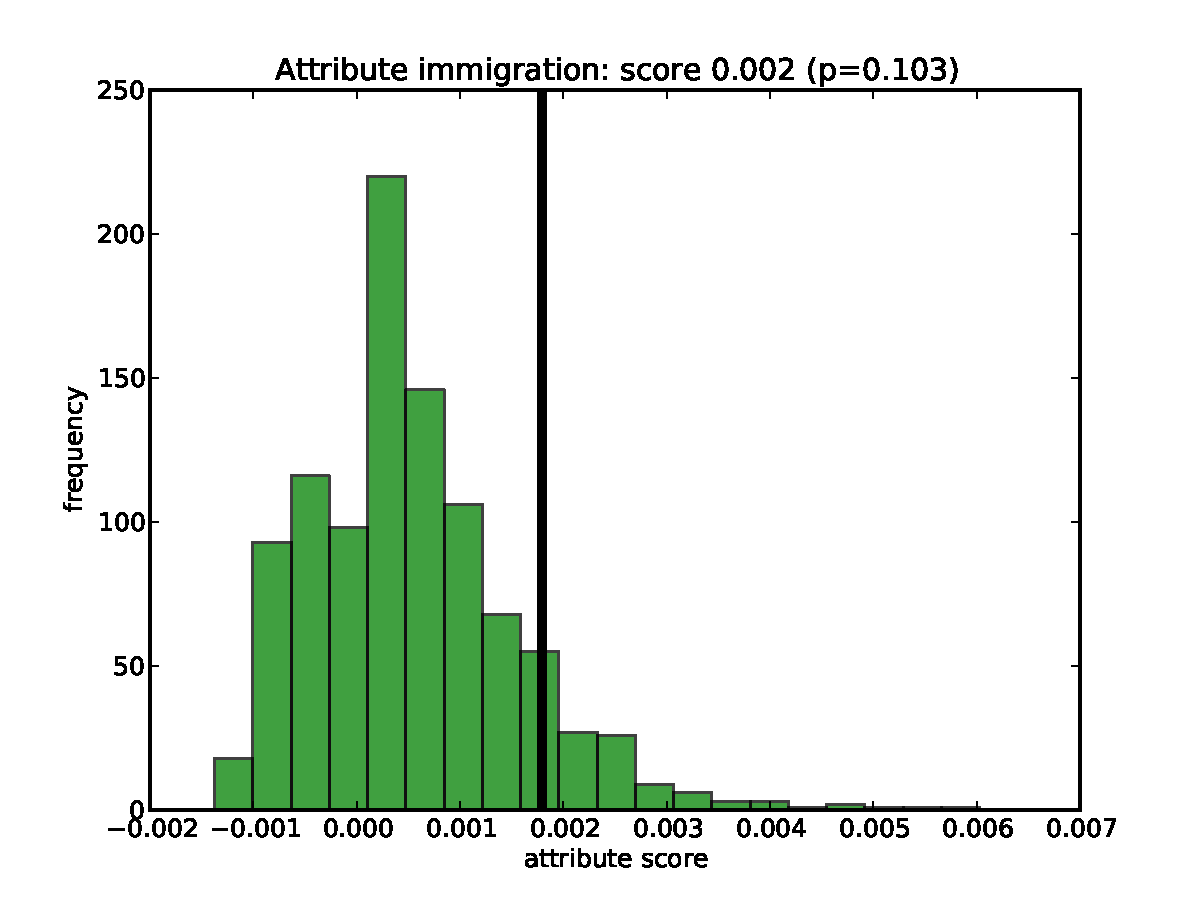
\includegraphics[width=8cm]{slike/att-score-null.pdf}
\caption{Rezultat permutacijske analize. Prikazana je porazdelitev informativnosti atributa, kot bi jo opazili, če bi bil razred primera naključen. Informativnost atributa na dejanskih, nenaključnih podatkih prikazuje vertikalna črta. Kar $10,3\%$ zmerjenih informativnost na naključnih podatkih je od te večja, zato tega atributa pri nadaljnji analizi ne bomo upoštevali.}
\label{f-att-score-null}
\end{center}
\end{figure}

Risanje grafov, kot je ta s slike~\ref{f-att-score-null}, je tipično zanimivo in informativno. Nikoli ne smemo zaupati samo golim številkam. Grafične ilustracije raznih analiz nam vedno pomagajo globlje razumeti problemsko domeno, čeprav vsi grafi niso ravno tisti, ki jih bomo vključili v naše končno poročilo. Da bo risanje takih grafov enostavneje, kodo za zgornji graf podajamo spodaj.

\begin{python}
import matplotlib.pyplot as plt

# plot score vs. null distribution for k-th worst attribute
k = 1
att, p = sorted(ps.items(), key=itemgetter(1), reverse=True)[k]
plt.close() # clear the drawing canvas
plt.hist(null[att], 20, facecolor="green", alpha=0.75)
plt.axvline(x=scores[att], color="k", linewidth=4)
plt.xlabel("attribute score")
plt.ylabel("frequency")
plt.title("Attribute %s: score %5.3f (p=%5.3f)" % (att.name, scores[att], p))
plt.savefig("att-score-null.pdf")
\end{python}

\section{Klasifikacijska drevesa}

Klasifikacijska drevesa so ena najbolj osnovnih in enostavnih orodij za gradnjo napovednih modelov pri problemih z diskretnim razredom. Ker ste ta algoritem že dobro spoznali pri uvodnih predavanjih iz umetne inteligence, tu le na kratko. Osnovna ideja algoritma je razbitje začetne množice podatkov na čim bolj (razredno) čiste podmnožice. Za razbitje uporabimo en sam atribut, razbitje pa izvedemo na podlagi njegovih vrednosti. Tako smo na sliki~\ref{f-squares-triangles} za razbitje množice likov uporabili informacijo o njihovi barvi. Ker tipično podatki vsebujejo več atributov, izberemo tistega, ki vodi k najbolj čistim podmnožicam, to je tistega, katerega informativnost je za dano množico primerov največja. V osnovnem algoritmu postopek ponavljamo na dobljenih podmnožicah vse dokler te niso čiste, ali pa dokler nismo uporabili že vse atribute.

Rekurzivni algoritem zgradi drevo s korenom drevesa, v katerem smo imeli vse učne primere. Korenu sledijo vozlišča -- njegovi neposredni nasledniki, kjer smo primere iz osnovne množice razdelili skladno z vrednostmi najbolj informativnega atributa na podmnožice. Postopek smo ponovili vse do listov drevesa. Listom pripadajo primeri, ki izpolnjujejo pogoje oziroma imajo vrednosti atributov podane tako, kot je to zapisano na poti od lista do korena drevesa. Za vsak list lahko iz pripadajočih primerov ocenimo, kateri razred je najbolj pogost. Pravimo, da list uvršča v ta razred. Za potrebe uvrščanja se zato, glede na atributne vrednosti danega primera, sprehodimo od korena navzdol vse do lista, ki nam določa ustrezno uvrstitev.

Zgoraj smo opisali osnovni algoritem, tako imenovan algoritem ID3~\cite{} za gradnjo dreves. V izboljšanih verzijah algoritma pa lahko uporabimo tudi nekaj dodatnih trikov:
%
\begin{description}
\item[Obravnava zveznih atributov.] Te v danem vozlišču nadomestimo z binarnim atributom tako, da poiščemo mejo $t_X$, kjer skupina primerov razpade na skupino, kjer je $X<t_X$ in kjer je $X>=t_X$. Mejo $t_X$ izberemo tako, da vrednosti tega atributa, ki jih uporabljajo primeri, za katere iščemo razbitje, uredimo in preiščemo vse točke na sredini med dvemi zaporednimi vrednostmi. Izberemo tako mejno vrednost, kjer je informativnost (ocena) dobljenega binarnega atributa najvišja. Postopek imenujemo tudi kategorizacija oz. diskretizacija atributa, in je lahko primeren za predobdelavo celotne množice učnih primerov pri situacijah, kjer uporabljene metode ne znajo neposredno uporabiti zveznih atributov.

\item[Obravnava neznanih vrednosti atributov pri gradnji drevesa.] Te lahko preprosto zanemarimo oziroma jih ne upoštevamo pri ocenjevanju verjetnosti. Lahko pa jih upoštevamo tako, da ocenimo verjetnosti posameznih vrednosti in primere z neznanimi vrednostmi ustrezno ``razpršimo'' po podmnožicah.

\item[Neznane vrednosti atributov in uvrščanje.] Pri uvrščanju primerov, pri katerih nekateri atributi nimajo danih vrednosti (pravimo, da so te vrednosti neznane), lahko naletimo na vozlišče, ki zahteva poznavanje enega od teh atributov. Uvrstitev poiščemo tako, da se spustimo po vseh njegovih vejah in v vsaki poiščemo ustrezni razred, ki ga utežimo z verjetnostjo vrednosti atributa v danem vozlišču. Slednjo seveda dobimo pri učenju drevesa in si jo moramo v vozlišču, za namene uvrščanja, zapomniti.

\item[Rezanje dreves.] Drevesa tipično vodijo k drobljenju oziroma fragmentaciji problemske domene. Na razred namesto iz celotne množice primerov sklepamo iz veliko manjših podmnožic, ki pa s stališča statistike niso nujno ustrezne (bi bilo prav o pravičnosti igralne kocke razmišljati že po nekaj metih?). Bolje bi zato bilo zgraditi drevesa tako, da ta ne vodijo k premajhnim množicam v listih. Postopek se imenuje rezanje dreves. Lahko ga izvajamo vnaprej (na primer, postavimo mejo za najmanjše število primerov v listih), ali pa vzvratno tako, da zgradimo drevo in potem rekurzivno odstranjujemo nezanesljiva spodnja vozlišča. Eden od znanih postopkov za slednje imenujemo rezanje z zmanjševanjem napake \angl{minimal error prunning} in temelji na spremenjenem ocenjevanju verjetnosti tako, da pri njej upoštevamo še nekaj navideznih primerov, po enega iz vsakega razreda (t.im. ocena po Laplace-u~\cite{}) ali pa $m$ primerov, ki so porazdeljeni skladno z porazdelitvijo razredov v učni množici (t.im. $m$-ocena verjetnosti~\cite{}).

\item[Združevanje vrednosti atributov.] Nekateri diskretni atributi uporabljajo lahko (zelo) veliko število vrednosti in bi njihova uporaba pri gradnji dreves lahko vodila v takojšnjo veliko razpršitev primerov. Zato raje te vrednosti uredimo v podmnožice, ki jih poiščemo tako, da ima tako dobljeni atribut največjo informativnost. Zakaj za ocenjevanje slednje osnovna mera z informacijskim prispevkom ni primerna?
\end{description}

Tehnika gradnje in uporabe klasifikacijskih dreves ima vrsto prednosti. Je sorazmerno hitra, enostavna, zna obravnavati kakršnekoli podatke, ki jih lahko zapišemo v atributni obliki, deluje tudi na zelo velikih množicah podatkov. Uvrščanje je hitro. Model je odprt, ter ga je moč enostavno vizualizirati (slika~\ref{f-titanic-tree}) in ob njem razpravljati o možnih vzorcih v podatkih, ki jih je algoritem odkril.

\begin{figure}[htbp]
\begin{center}
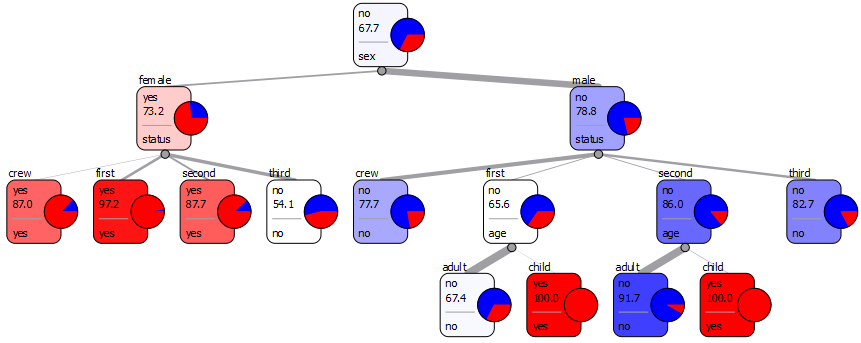
\includegraphics[width=15cm]{slike/titanic-tree.png}
\caption{Klasifikacijsko drevo zgrajeno iz podatkov o potnikih na ladji Titanic. Razred govori o preživetju nesreče. Debelina povezav med vozlišči drevesa ustreza številu primerov na teh povezavah. Barva vozlišč govori o verjetnosti prevladujočega razreda.}
\label{f-titanic-tree}
\end{center}
\end{figure}

Klasifikacijska drevesa pa imajo tudi pomanjkljivosti. O problemu fragmentacije, ki omejuje splošnost dreves in povzroči, da drevo sklepa o razredu na premajhnem vzorcu primerov, smo že govorili (kje? kdaj?). Tudi predstavljeni algoritem ne odkrije optimalnega drevesa, saj ne implementira vračanja in s tem kompleksnejše optimizacije. Drevesa so lahko izjemno velika in se lahko hitro preveč prilagodijo učnim podatkom. V splošnem drevo lahko modelira kompleksnejše povezave med primeri, na primer tudi take iz tabele~\ref{t-xor-boat}, a njih odkritje je pri uporabi univariatnih mer prepuščeno zgolj precej neverjetnemu naključju. Seveda pa lahko gradnjo dreves usmerjamo tudi s kontekstnimi merami kot je ReliefF, a s tem močno upočasnimo postopek gradnje.

Drevesa so prav tako občutljiva na lahko zelo majhne spremembe v učni množici. Prav lahko se zgodi, da sta dva ali več atributov med seboj zelo primerljiva po informacijski vsebini, in da majhne spremembe vplivajo na to, kateri atribut bomo izbrali. To situacijo lahko opazimo v korenu ali pa kakšnem drugem od notranjih vozlišč. V obeh primerih so lahko spremembe v strukturi drevesa izjemno velike, še posebej, če gre za vozlišče blizu vrha drevesa. Ta občutljivost je seveda nezaželena. Domenskim ekspertom bi želeli pokazati model, ki je stabilen, in se ne spreminja ob najmanjši spremembi učne množice. Izkorišča pa jo tehnika, o kateri govorimo spodaj.

\section{Naključni gozd}

Naključni gozd \angl{random forest} v uvrščanju sestavlja skupina klasifikacijskih dreves, ki pri klasifikaciji primera v razred glasuje~\cite{}. Naključni gozd napove razred, kamor primer uvršča večina klasifikacijskih dreves, ki gozd sestavlja. Najbolje bi bilo, da gozd sestavljajo drevesa, ki so med seboj različna in kjer vsak od dreves odkrije kakšen svoj, zanimiv koncept, ki se je skrival v podatkih. Podatke ti modeli osvetlijo iz različnih strani in potem skupaj o razredu glasuje. Več dreves več ve.

Taka drevesa dobimo v gozdu tako, da postopek malo ``ponaključimo''. In sicer:
\begin{enumerate}
\item Pričnemo z učno množico $D$, ki vsebuje $N$ primerov in $M$ atributov.
\item Izberemo število $m$, ki nam pove, med koliko naključno izbranih atributov iz primerov v vozliščih drevesa bomo izbrali najboljšega. Število $m$ naj bo veliko manjše od števila atributov, na primer $m=\sqrt{M}$. Izberemo tudi število dreves $K$ v gozdu, na primer $K=100$, ki ga želimo zgraditi. Nastavimo števec dreves, $i\leftarrow 1$.
\item Med $N$ primeri učne množice $D$ naključno z vračanjem izberemo novo množico primerov $D_i$ enake velikosti. To vrsto vzorčenja imenujemo metoda stremena \angl{bootstrap}. Seveda bodo v našem vzorcu posamezni primeri iz osnovne učne množice podvojeni.
\item Na množici primerov $D_i$ zgradimo klasifikacijsko drevo $T_i$, a tako, da v vsakem vozlišču naključno izberemo $m$ atributov, ki so uporabljeni v primerih vozlišča, in med njimi za delitev teh primerov izberemo najbolj informativnega upoštevaje razred primerov.
\item Če $i==K$ smo končali, sicer $i\leftarrow i+1$ in nazaj na korak 3.
\end{enumerate}

Tehnika naključnega gozda je danes ena od najbolj zanesljivih tehnik uvrščanja. Njene napovedne točnosti so tipično med najboljšimi. Tehnika podeduje vse prednosti klasifikacijskih dreves, zgubi pa možnost interpretacije modela, saj tega sedaj sestavlja vrsta modelov katerih vpliv na odločitve ni jasen in je odvisen od konteksta. Pristop v fazi gradnje modela ni med najhitrejšimi, ga pa je enostavno povzporediti.

Brieman~\cite{} je ob tem, ko je predlagal algoritem za gradnjo naključnega gozda, predlagal tudi metodo, ki oceni pomembnost, ki jo v gozdu imajo posamezni atributi pri pravilnem uvrščanju. Vsakemu vzorcu primerov $D_i$, na katerem smo zgradi drevo $T_i$,  določimo njegov komplement $D_i'=D-D_i$. Množica $D_i'$ je torej sestavljena iz primerov osnovne učne množice $D$, ki jih ni v vzorcu $D_i$ \angl{out-of-bag set}. Naj bo $C_i$ število primerov iz množice $D_i$, za katere je drevo $T_i$ pravilno napovedalo razred. Sedaj za vsak atribut $X$ premešajmo njegove vrednosti v $D_i$ in na taki, spremenjeni množici, izmerimo število pravilnih napovedi $C_{i,X}$. Pomembnost \angl{raw importance} atributa določimo kot:
%
$$ {\rm RI}(X)= {1\over K}\sum_{i=1}^K{C_i - C_{i,X}} $$


\chapter{Priporočilni sistemi}

Priporočilni sistemi so danes v računalništvu in informatiki prisotni
praktično povsod. Še najbolj očitno se z njimi srečamo pri obisku
raznih spletnih strani, kot so Facebook, eBay, Amazon, IMDB, Netflix in podobnih. Te strani si vneto beležijo podatke o naših obiskih, ogledu izbranih podstrani, kupljenih izdelkih, ki jih strani ponujajo, ali pa odzivih na ponujene informacije (so nam te všeč ali ne?). Samo na podlagih naših podatkov bi te strani ne bile preveč ``pametne''. A ker se tam zbirajo podatki tudi o vseh ostalih obiskovalcih, je lahko na ta način zbranih informacij hitro dovolj. ``Inteligenco'' te strani kažejo v vsebinah, ki so prilagojene nam, uporabnikom. Strani nam svetujejo, kaj vse bi se nam splačalo pogledati, katere izdelke ali druge strani bi lahko bile zanimive in kaj nasploh lahko še počnemo glede na naše, največkrat implicitno izražene interese.

Jedro takih spletnih strani, programov in sistemov so priporočilni sistemi. Ti
lahko na podlagi zbranih informacij o uporabnikih sklepajo o uporabnikovih preferencah, željah in interesih. Za posameznega uporabnika lahko recimo na podlagi njemu podobnih uporabnikov napovedo, kaj bi uporabnika lahko (še) zanimalo in mu ponudijo ogled stvari, ki jih ta do sedaj še ni pogledal, pa bi ga morda lahko navdušile. Uporabnost in privlačnost teh priporočilnih storitev ter posledično njihova finančna uspešnost je lahko zelo odvisna od kvalitete uporabljenih priporočilnih sistemov oziroma temu, kako dobro ti modelirajo dejanske uporabnikove interese.

Priporočilni sistemi so lahko uporabni v trženju, analitiki in priporočanju v socialnih omrežjih, biomedicini, humanistiki, astronomiji, kemiji -- pravzaprav jih lahko uporabimo prav na vseh področjih, kjer se zbirajo podatki o uporabnikih in stvareh, ki jih neka spletna stran ali programskih sistem, ali pa dejanska fizična trgovina ponuja. V tem poglavju se bomo osredotočili na priporočilne sisteme, ki delujejo na preferencah, ki so jih uporabniki eksplicitno ali implicitno podali o množici stvari. Ko govorimo o ``stvareh'' mislimo na izdelke, spletne strani, filme, glasbo, kakršnekoli koncepte, torej na karkoli, o čemer so se uporabniki preko neke storitve ali spletne strani izrekli. Stvari so uporabniku lahko bile všeč ali ne, lahko jih je številčno ocenil, morda samo označil zanimive izdelke. Lahko pa si je sistem samo zapomnil, katere spletne strani ali storitve je uporabnik izbral, katero glasbo je poslušal ali kateri film si je ogledal. Vrsto priporočilnih sistemov, ki temelji na takem preferenčnem znanju in pri podajanju priporočil uporablja uporabniške profile vseh ostalih uporabnikov v sistemu imenujemo skupinsko filtriranje \angl{collaborative filtering}.

Čeprav bomo v tem poglavju govorili samo o skupinskem filtriranju, naj
tu omenimo, da obstajajo tudi drugačni pristopi k priporočanju. Na
spletu recimo lahko najdemo sezname najboljših izdelkov določenega
tipa, ki jih je priporočil nek urednik ali pisatelj bloga. Spletne
strani, kot so na primer domača enaa.com, nam na vhodni strani
predlaga izdelke, ki so najbrž izbrani med najbolj dostopanimi ali pa
so bili v preteklem obdobju s strani vseh uporabnikov najbolje
ocenjeni. Tu gre za enostavno združevanje ocen uporabnikov, ali pa
uporabo enostavnih postopkov štetja dostopov uporabnikov do izdelkov.

Uporabimo lahko tudi dodatna znanja o uporabnikih in stvareh. Uporabnike lahko opišemo s starostjo, spolom, naštejmo interesna področja, ki jih zanimajo, opišemo, kaj delajo v službi, kakšni so njihovi hobiji, ali pa celo s kom se družijo. Stvarem lahko določimo njihov namen, jih opremimo s ključnimi besedami iz opisa, razvrstimo v razne skupine. Na podlagi teh podatkov lahko priporočilni sistemi sklepajo o nam podobnih uporabnikih ali pa stvareh, ki so podobne tem, ki smo jih že pozitivno ocenili. Priporočilne sisteme, ki temeljijo na takem dodatnem poznavanju uporabnikov in stvari \angl{knowledge-based recommendation systems} je morda, zaradi potrebnih dodatnih podatkov, je tipično težje vzpostaviti od sistemov skupinskega filtriranja, njihova točnost pa je presenetljivo lahko celo slabša od točnosti slednjih. Uporaba metod, ki uporabljajo dodatna znanja o uporabnikih in stvareh, je lahko ključna pri hladnem zagonu sistema \angl{cold start}, ko uporabnik storitve še ni uporabljal in zanj še nimamo nimamo podatkov o preferencah oziroma všečnosti stvari, na katerih bi temeljila priporočila skupinskega filtriranja.

V nadaljevanju spregovorimo torej samo o tehnikah skupinskega filtriranja. Priporočilnim sistemom, ki uporabljajo dodatna znanja, se izognemo, bo pa radovedni bralec lahko sam razpoznal, da bi bilo moč te tehnike enostavno razviti in pri tem uporabiti zelo podobne koncepte kot pri skupinskem filtriranju. Oba pristopa namreč temeljita na ocenjevanju podobnosti med uporabniki in med stvarmi, razlikujeta se le v načinu, kako te podobnosti izračunamo in v podatkih, ki jih za to uporabimo.

\section{Podatki}

Naš cilj je razviti priporočilni sistem za skupino uporabnikov $\mathcal{U}$, ki lahko izbirajo med množico stvari $\mathcal{I}$, kjer bomo imeli $N$ različnih uporabnikov ($|\mathcal{U}|=N$) in $M$ različnih stvari ($\mathcal{I}=M$). Preferenčno znanje $\mathcal{R}$ bomo zapisali kot množico trojk $(u,i,r)$ za uporabnika $u\in\mathcal{U}$, stvar $i\in\mathcal{I}$ in preferenco $r$, ki bo podala ocena oziroma zaželenosti stvari $i$ s strani uporabnika $u$.

Preference merimo v neki izbrani merski lestvici. Na primer, ocene zapišemo s celimi števili od 1 do 5, ali pa od 0 do 10, ali pa z realnimi števili od 0.0 do 1.0 ali pa od -1.0 do 1.0. Včasih pa imamo na voljo samo oznake, ali je uporabnik za določeno stvar izrazil zanimanje. Slednji primer je težji, saj nimamo urejenih ocen oziroma imamo samo označene pozitivne preference. Predpostavka, da so vse stvari, ki jih uporabnik ni označil, zanj nezanimive, pa je lahko napačna. V tem poglavju se bomo predvsem ukvarjali s podatki, kjer imamo na voljo numerične ocene, tu in tam pa bomo namignili, kako bi lahko obravnavali podatki, ki vsebujejo samo seznam zanimivih stvari, za katere uporabnik ni podal preferenčne ocene v neki numerični lestvici.

Priporočilne sisteme lahko razvijamo za manjše skupine uporabnikov in stvari, opravka pa imamo lahko tudi z večjimi množicami, kjer je lahko število uporabnikov in stvari tudi po več tisoč, sto tisoč ali pa celo nekaj milijonov. Celotno preferenčno znanje, torej ocene za vse kombinacije uporabnikov in stvari tako ne bo nikoli dostopno, opravka pa bomo imeli samo z manjšim vzorcem preferenčnega znanja, ki ga označimo s $\tau'\subset\mathcal{R}$. Ker bomo na podlagi tega vzorca zgradili naš priporočilni sistem, ga tu imenujmo učna množica. Predpostavili bomo, da obstaja največ ena ocena za vsako kombinacijo $(u, i)$, torej kombinacijo uporabnik-stvar. Ker se bomo še največkrat spraševali o tem, ali naša učna množica vsebuje oceno za dan par $(u,i)$, uvedimo množico parov $\tau$, za katere imamo dano preferenčno znanje:
%
$$\tau=\{(u,i); \exists r:(u,i,r)\in\tau'\}$$
%
Preferenčno oceno uporabnika $u$ za stvar $i$ zapišimo z $r_{u,i}$. Množica ocen izbranega uporabnika $u$ tvori uporabniški profil ${\bf r}_u$. Podobno lahko vse ocene uporabnikov za izbrano stvar $i$ zberemo v stvarni profil oziroma profil stvari ${\bf r}_i$.

Primer s seznamom podanega preferenčnega znanja podaja tabela~\ref{t:pref-ocene}, kjer so
\begin{eqnarray}
{\mathcal U} & = & \{ {\rm Mojca}, {\rm Miha}, {\rm Sandra}, {\rm Jana}, {\rm Tina}, {\rm Nik}, {\rm Janez}, {\rm Cene} \} \nonumber \\
{\mathcal I} & = & \{ {\rm olive}, {\rm vampi}, {\rm testenine}, {\rm blitva}, {\rm ocvirki}, {\rm krofi} \} \nonumber
\end{eqnarray}

\begin{table}
\caption{Primer preferenčnega znanja podanega kot množica trojk (uporabnik, stvar, ocena).}
\label{t:pref-ocene}
\begin{center}
\small
\begin{tabular}{lll}
\toprule
uporabnik & izdelek & ocena \\
\midrule
Mojca & olive & 5.0 \\
Mojca & vampi & 1.2 \\
Mojca & testenine & 4.1 \\
Mojca & blitva & 5.0 \\
Miha & ocvirki & 4.3 \\
Miha & vampi & 4.9 \\
Miha & blitva & 1.2 \\
Sandra & ocvirki & 2.3 \\
Sandra & olive & 5.0 \\
Sandra & vampi & 0.1 \\
Sandra & blitva & 5.0 \\
Jana & ocvirki & 4.0 \\
Jana & vampi & 3.0 \\
Jana & krofi & 4.5 \\
Tina & olive & 5.0 \\
Tina & krofi & 3.5 \\
Tina & testenine & 2.1 \\
Tina & blitva & 4.6 \\
Nik & ocvirki & 2.0 \\
Nik & olive & 3.8 \\
Nik & vampi & 0.3 \\
Janez & olive & 0.3 \\
Janez & vampi & 4.8 \\
Janez & testenine & 2.5 \\
Cene & ocvirki & 3.9 \\
Cene & krofi & 4.8 \\
Cene & blitva & 3.0 \\
\bottomrule
\end{tabular}
\end{center}
\end{table}

Namesto podajanja preferenčnega znanja oziroma naše učne množice s trojkami (uporabnik, stvar, ocena) bi lahko, konceptualno, to znanje zapisali v obliki matrike (tabela~\ref{t:pref-matrika}). ``Konceptualno'' namreč zato, ker bi za večjo skupino uporabnikov in stvari take matrike postale izjemno velike in ker jih kot take, v resnih računalniških implementacijah, nikoli eksplicitno ne uporabimo, ampak namesto njih podatke zapišemo v slovarje.

\begin{table}
\caption{Primer preferenčnega znanja podanega z matriko}
\label{t:pref-matrika}
\begin{center}
\begin{tabular}{lcccccc}
\toprule
& olive & vampi & testenine & blitva & ocvirki & krofi \\
\midrule
Mojca & 5.0 & 1.2 & 4.1 & 5.0 & & \\
Miha & 4.3 & 4.9 & & 1.2 & & \\
Sandra & 5.0 & 0.1 & & 5.0 & 2.3 & \\
Jana & & 3.0 & & & 3.0 & 4.5 \\
Tina & 5.0 & & 2.1 & 4.6 & & 3.5 \\
Nik & 3.8 & & & & 2.0 & \\
Janez & 0.3 & 4.8 & 2.5 & & & \\
Cene & & & & 3.0 & 3.9 & 4.8 \\
\bottomrule
\end{tabular}
\end{center}
\end{table}

\section{Skupinsko filtriranje na podlagi podobnosti}

Skupinsko filtriranje \angl{collaborative filtering} je danes ena od osnovnih, morda glavnih tehnik za izdelavo praktičnih priporočilnih sistemov, ki temeljijo na preferenčnem znanju množic uporabnikov. Za danega uporabnika v teh sistemih predpostavimo, da je ta že ocenil določene stvari. Priporočilo, katera stvar ga bi zanimala med temi, za katere še ni podal preference, pridobimo tako, da za vse take stvari izračunamo pripadajočo oceno (preferenco) ter uporabniku priporočimo stvar, ki je bila na ta način najbolje ocenjena. Priporočila za danega uporabnika razvijemo ob predpostavki, da je v celotni množici uporabnikov nekaj takih, ki so izbranemu uporabniku podobni. Stvari, ki so všeč njim, bodo najbrž všeč tudi izbranemu uporabniku. 

Najbolj neposreden način, ki se ga pri napovedovanju ocen lahko poslužimo je, da na podlagi že danih ocen izračunamo, kako podobni so med seboj uporabniki ter ocene ostalih uporabnikov za posamezno stvar utežimo s podobnostjo ciljnemu uporabniku. 

\subsection{Podobnost med uporabniki}

Za danega uporabnika $u$ nas zanima, kako podobni so mu ostali uporabniki. Določiti moramo mero podobnosti med uporabniškimi profili. Spomnimo se: uporabniški profil je množica vseh ocen stvari, ki jih je uporabnik ocenil oziroma za katere imamo podatke v učni množici. Nekaj kandidatov za mere podobnosti poznamo že iz prejšnjih poglavij, zato tu le na hitro omenimo, da je primerna in mnogokrat uporabljana mera kosinusne podobnosti:
%
$$ s_{\rm c}(u,u')={{\bf r}_u {\bf r}_{u'} \over |{\bf r}_u|\ |{\bf r}_{u'}|}$$
%

Pri kosinusni podobnosti manjkajoče podatke izpustimo. Ko računamo razdaljo med Mojco in Mihom, na primer, bomo upoštevali samo ocene za olive, vampe in blitvo. Njuna profila za te tri stvari bosta zato $(5.0, 1.2, 5.0)$ in $(4.3, 4.9, 1.2)$. Skalarni produkt teh dveh vektorjev znaša $33.38$, njuni dolžini sta $7.17$ in $6.62$, torej je njuna kosinusna podobnost enaka $0.7$. Podobnost med Mojco in Tino (vektorja, ki ju primerjamo, sta $(5.0, 1.2, 5.0)$ in $(5.0, 2.1, 4.6)$) je večja in znaša $0.99$. Opazimo tudi lahko, da bo recimo podobnost med Janezom in Cenetom enaka $0.0$, saj ne obstaja izdelek, ki bi ga ta dva uporabnika oba ocenila.

V primeru, da preferenčnih ocen nimamo in uporabniške profile tvori samo seznam stvari, ki so uporabniku všeč, lahko oceno podobnosti med uporabniki izračunamo z mero po Jaccardu:
%
$$ s_{\rm J}(u, u')={||{\bf r}_u\cap{\bf r}_{u'}|| \over ||{\bf r}_u\cup{\bf r}_{u'}||}$$
kjer smo, na primer, z $||{\bf r}_u\cap{\bf r}_{u'}||$ označili število stvari, ki so všeč tako uporabniku $u$ kot uporabniku $u'$.

\subsection{Priporočila na podlagi uporabniških profilov in podobnosti med uporabniki}

Za danega uporabnika $u$ želimo z uporabo učnih podatkov oceniti, kakšna je njegova preferenčna ocena za stvar $i$. To označimo z $\hat{r}_{ui}$, saj gre za oceno oziroma približek. Preferenčno oceno lahko na ta način pridobimo tudi za že obstoječo oceno iz učne množice, a bo ta verjetno različna od ocene $r_{ui}$, ki jo je podal uporabnik in bomo pri njeni napovedi storili določeno napako.

Izhodišče za izračun preference $\hat{r}_{ui}$, torej ocene koristnosti stvari $i$ za uporabnika $u$ so podobnosti med uporabniki. Ideja pa je enostavna: pogledamo, kdo so vsi uporabniki, ki so ocenili stvar $i$. Njihove ocene utežimo s podobnostjo s ciljnim uporabnikom $u$ ter dobljeno vsoto normirano z vsoto uteži:

\begin{equation}
\hat{r}_{ui} = \frac{\displaystyle\sum_{u':(u',i)\in\tau,\ u'\neq u}s(u,
  u')\times r_{u'i}}{\displaystyle\sum_{u':(u',i)\in\tau,\ u'\neq u}s(u, u')}
\end{equation}

\subsection{Priporočila na podlagi profilov stvari in podobnosti med stvarmi}

Tudi stvari imajo svoje profile. Če so uporabniški profili vrstični vektorji v preferenčni matriki, katere primer je prikazan v tabeli~\ref{t:pref-matrika}, so profili stvari stolpci te matrike, oziroma stolpčni vektorji. Za stvar $i$ njen profil zapišemo z ${\bf r}_i$. Podobno kot za dva uporabnika lahko podobnost med stvarmi merimo, na primer s kosinusno razdaljo:
%
$$ s_{\rm c}(i,i')={{\bf r}_i {\bf r}_{i'} \over |{\bf r}_i|\ |{\bf r}_{i'}|}$$
%

Sedaj pa nazaj k priporočanju. Želeli bi torej oceniti preferenco $\hat{r}_{ui}$, ki jo ima za stvar $i$ uporabnik $u$. Predpostavljamo, da je uporabnik že ocenil nekaj drugih stvari (vsako od teh bomo označili z $i'$). Oceno za stvar $i$ lahko izračunamo iz teh ocen, a pri tem močneje upoštevamo tiste stvari, ki so podobne stvari $i$, ki jo ocenjujemo:
%
\begin{equation}
\hat{r}_{ui} = \frac{\displaystyle\sum_{i':(u,i')\in\tau,\ i'\neq i}s(i,
  i')\times r_{ui'}}{\displaystyle\sum_{i':(u,i')\in\tau,\ i'\neq i}s(i, i')}
\end{equation}

Ta izračun je na moč podoben izračunu iz prejšnjega razdelka, le da tu utežimo ocene našega ciljnega uporabnika, v prejšnjem razdelku pa smo utežili ocene ostalih uporabnikov.

\subsection{Priporočanje na podlagi podobnosti uporabnikov in stvari}

Priporočilno tehniko iz prejšnjih dveh podpoglavij lahko združimo. Iz učne množice lahko vzamemo poljubno oceno $r_{u'i'}$ ter jo utežimo glede na podobnost s ciljnim uporabnikom $u$ in ciljno stvarjo $i$, za katero oceno $\hat{r}_{ui}$ iščemo. Utežena vsota vseh teh ocen je naš približek za $\hat{r}_{ui}$:
%
\begin{equation}
\hat{r}_{ui} = \frac{\displaystyle\sum_{(u',i')\in\tau,\ (u',i')\neq (u,i)}s(u,u')\times s(i, i')\times r_{u'i'}}{\displaystyle\sum_{(u',i')\in\tau,\ (u',i')\neq (u,i)}s(u,u')\times s(i, i')}
\end{equation}

Na prvi pogled se nam taka rešitev lahko zazdi še najboljša, oziroma bolj primerna od teh, ki smo jih omenjali v prejšnjih dveh podpoglavjih. A njena očitna slabost je časovna kompleksnost, saj moramo poznati praktično vse pare podobnosti, torej med ciljnim in vsemi ostalimi uporabniki in ciljno in vsemi ostalimi stvarmi. V prejšnjih dveh podpoglavjih smo namreč računali na to, da so ciljno stvar $i$ ocenili samo nekateri uporabniki in je bilo potrebno izračunati podobnosti samo za te. Oziroma, računali smo, da je uporabnik $u$ ocenil samo manjši nabor stvari in da je samo te potrebno primerjati s ciljno stvarjo $i$.

\subsection{Priporočanje kar tako}

Vrednost $\hat{r}_{ui}$ lahko ocenimo kar s povprečno oceno stvari $i$ vseh (ostalih) uporabnikov, ki so to stvar ocenili:
%
\begin{equation}
\hat{r}_{ui} = \frac{\displaystyle\sum_{(u',i)\in\tau,\ u'\neq u} r_{u'i}}{|\{(u',i)\in\tau,\ i'\neq i \}|}
\end{equation}
%
Ta ocena bo neodvisna od uporabnika, nam pa lahko služi za primerjavo z ostalimi načini izračuna $\hat{r}_{ui}$, kot smo jih podali zgoraj. To oceno lahko morda še dodatno popravimo tako, da upoštevamo povprečno oceno uporabnika:
%
\begin{equation}
\hat{r}_{ui} = {1\over 2}\frac{\displaystyle\sum_{(u',i)\in\tau,\ u'\neq u} r_{u'i}}{|\{(u',i)\in\tau,\ i'\neq i \}|} + {1\over 2}\frac{\displaystyle\sum_{(u,i')\in\tau,\ i'\neq i} r_{ui'}}{|\{(u,i')\in\tau,\ i'\neq i \}|}
\end{equation}
%

\section{Pristranost}

Uporabniki smo v naših ocenah pristrani: nekateri uporabniki bolj
vedre narave bodo stvari ocenjevali z višjimi ocenami, nekateri
uporabniki pa bodo le stežka dajali najvišje ocene. Problemu
pristranosti uporabnikov se lahko vsaj deloma izognemo tako, da vsem
ocenam iz učne množice odštejemo povprečno oceno uporabnika. Se pravi
$r_{ui}$ nadomestimo z $r_{ui}-\overline{{\bf r}_u}$. Tako
popravljene ocene potem uporabimo pri učenju. Pri napovedovanju pa ne
smemo pozabiti, da smo povprečne ocene uporabnika pred tem odšteli, in
zato za par $(u,i)$ napovemo preferenčno oceno z
$\hat{r}_{ui}+\overline{{\bf r}_u}$.

\section{Ocenjevanje kvalitete priporočilnih sistemov}

Tudi tu lahko uporabimo prečno preverjanje, ki ga tokrat izvedemo kar nad množico trojk $(u,i,r_{ui})$. Torej tako, kot če bi vzorec iz tabele~\ref{t:pref-ocene} vzeli za učenje, na preostalem delu pa preverili naše izračunane preferenčne ocene. Za ocenjevanje kvalitete priporočanja lahko uporabimo iste mere, kot smo jih uporabili pri regresiji, torej na primer RMSE ali pa $R^2$.

\section{Priporočanje z matričnim razcepom}

V tabeli~\ref{t:pref-matrika} smo učne podatke predstavili kot matriko R, katere elementi so ocene $r_{ui}$ uporabnika $u$ za stvar $i$. Matrika R je redka, za njo pa mora priporočilni sistem znati oceniti vrednost manjkajočih elementov. Ker je uporabnikov $N$, stvari pa $M$, je matrika R oblike $M\times N$.Tipično sta dimenziji $M$ in $N$ visoki: uporabnikov je lahko nekaj tisoč, deset tisoč ali celo milijon, stvari pa ravno tako.

Že iz poglavja o gručenju vemo, da lahko stvari in uporabnike razvrstimo v skupine in za te potem poiščemo tipične stvari in tipične uporabnike. Na primer, pri izposoji filmov bi lahko zaznali, da obstajajo uporabniki storitve, ki radi gledajo večinoma akcijske filme, pa uporabniki, ki gledajo samo filme, ki so narejeni v Hollywoodu ter uporabniki, ki jim to ne pade na misel in si sposojajo samo umetniške filme iz manjših produkcijskih hiš. Uporabnike bi zato lahko predstavili s kratkimi profili, ki bi nam poročali o zaželenosti posameznih filmskih zvrsti. Pravimo, da bi na ta način uporabnike opisali v latentnem prostoru filmov, torej v prostoru filmskih kategorij, ki jih moramo iz podatkov šele razbrati. Po drugi strani pa bi tudi filme lahko opisali s profili v latentnem prostoru skupin uporabnikov, torej skupin, ki jih prav tako moramo šele pridobiti. Ta opis, predstavitev podatkov v latentnem, navideznem prostoru skupin stvari in skupin uporabnikov lahko pridobimo z enotnim postopkom, ki mu pravimo matrični razcep.

V pristopu z matričnim razcepom matriko ${\rm R}_{N\times M}$ predstavimo z matrikami ${\rm P}_{N\times K}$ in ${\rm Q}_{K\times M}$ tako, da velja ${\rm R}\approx {\rm P}{\rm Q}$ in da je $K<<M, N$ (slika~\ref{f:matricni-razcep}). Torej, tako, da je produkt matrik ${\rm P}$ in ${\rm Q}$ po elementih čim bolj podoben prvotni matriki ${\rm R}$ oziroma elementom, ki so tam definirani. Konstanta $K$ podaja število latentnih dimenzij, in je pri obliki razcepa, kot smo ga določili tu, enaka tako za uporabnike kot za stvari. Pravimo ji tudi stopnja razcepa. Ker je $K$ veliko manjši od dimenzij $M$ in $N$, v skrajnem primeru pa enak 1, pomeni, da s produktom ${\rm P} {\rm Q}$ prav gotovo ne bomo mogli verno predstaviti matriko $\rm R$, torej tako, da bi vsi elementi produkta bili enaki elementom vhodne matrike $\rm R$ (torej, ${\rm P}{\rm Q}\equiv {\rm R}$).

\begin{figure}[htbp]
\begin{center}
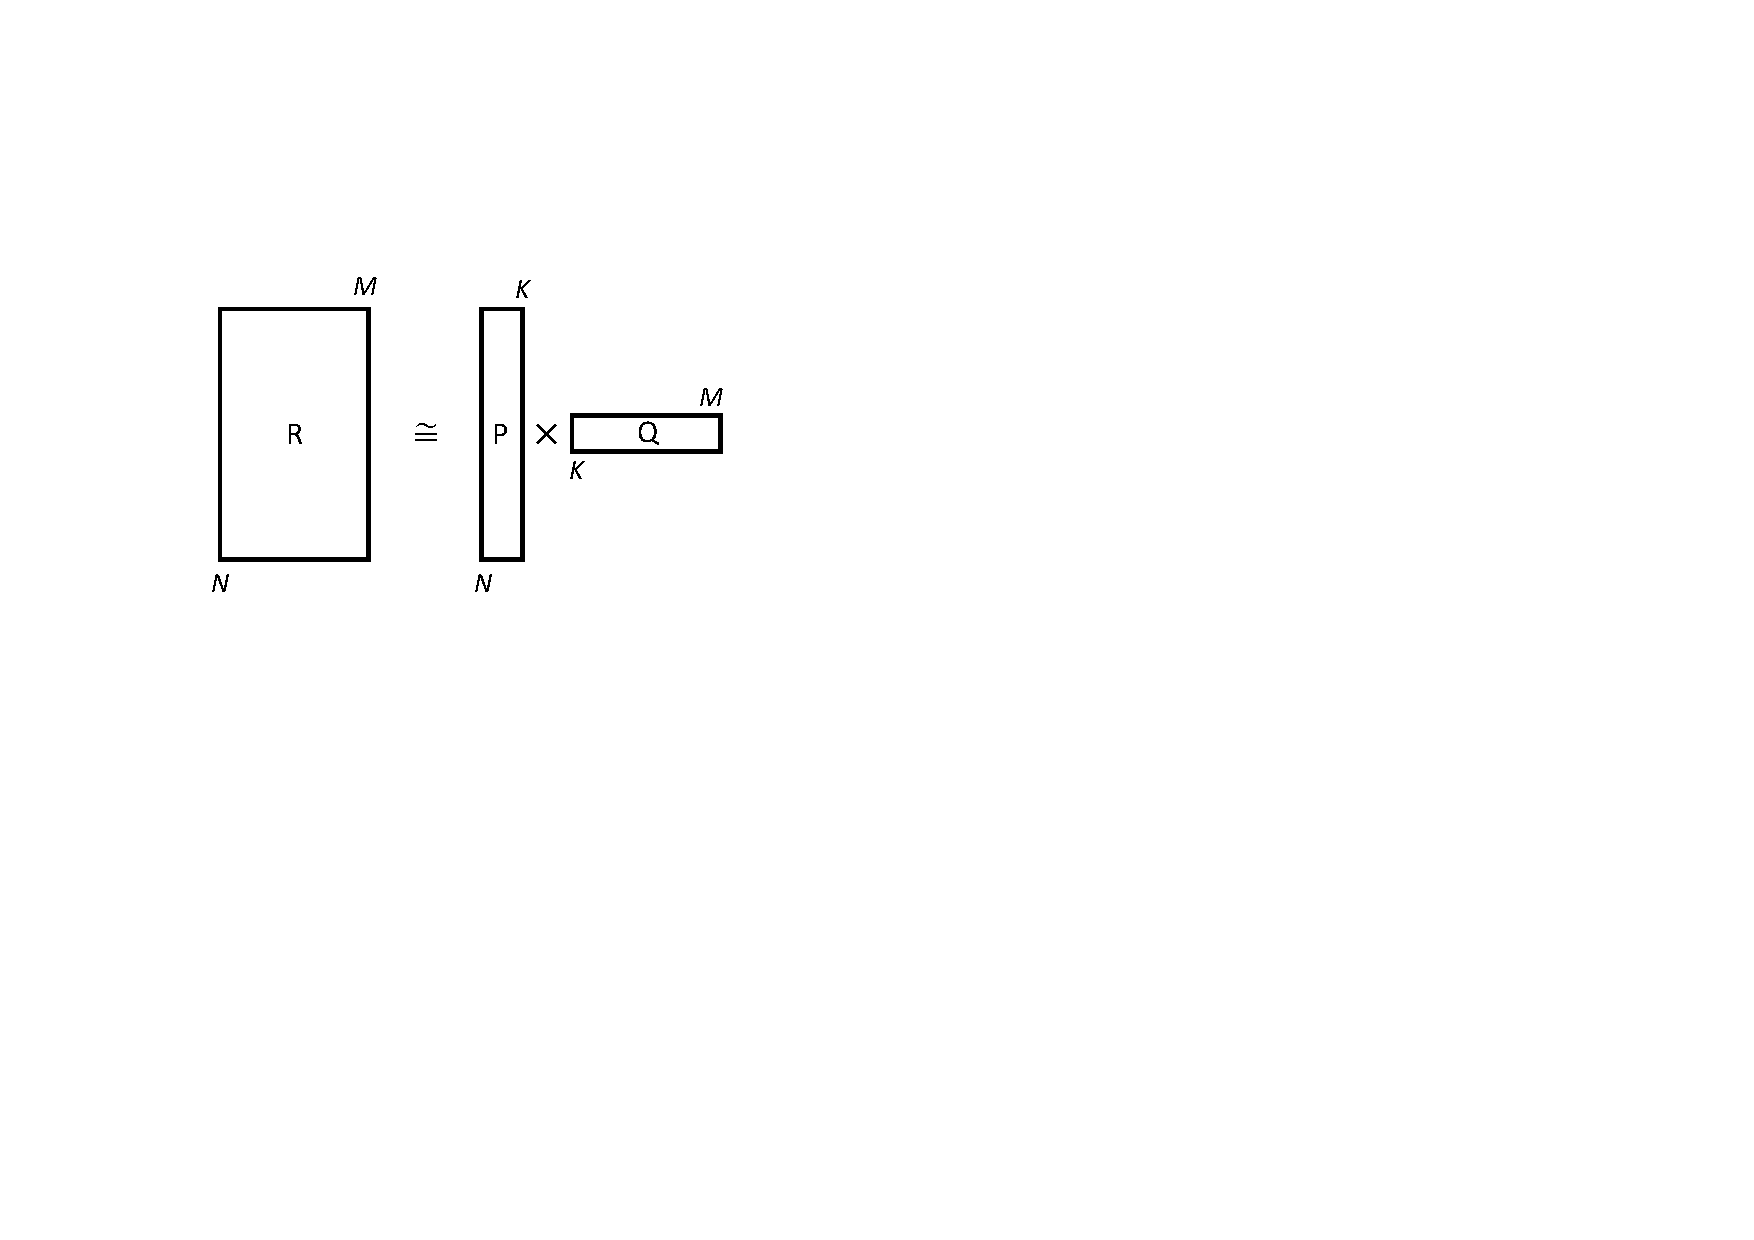
\includegraphics[width=7cm]{slike/matricni-razcep.pdf}
\caption{Razcep matrike R na manjši matriki P in Q.}
\label{f:matricni-razcep}
\end{center}
\end{figure}

Matrika $\rm P$ je matrika uporabniških profilov v latentnem prostoru filmov, torej prostoru tipičnih zvrsti filmov (teh nimamo, a jih pridobimo z razcepom matrike na produkt dveh matrik). Latentni profil uporabnika $u$ označimo z vektorjem ${\bf p}_u$. Podobno je matrika $\rm Q$ matrika profilov stvari v prostoru latentnih uporabnikov, profil stvari $i$ v tem prostoru pa zapišimo z vektorjem ${\bf q}_i$. Produkt latentnih profilov ustreza približku vrednosti ocene stvari $i$ uporabnika $u$, torej $\hat{r}_{ui}$ (slika~\ref{f:latentni-faktorji}).

\begin{figure}[htbp]
\begin{center}
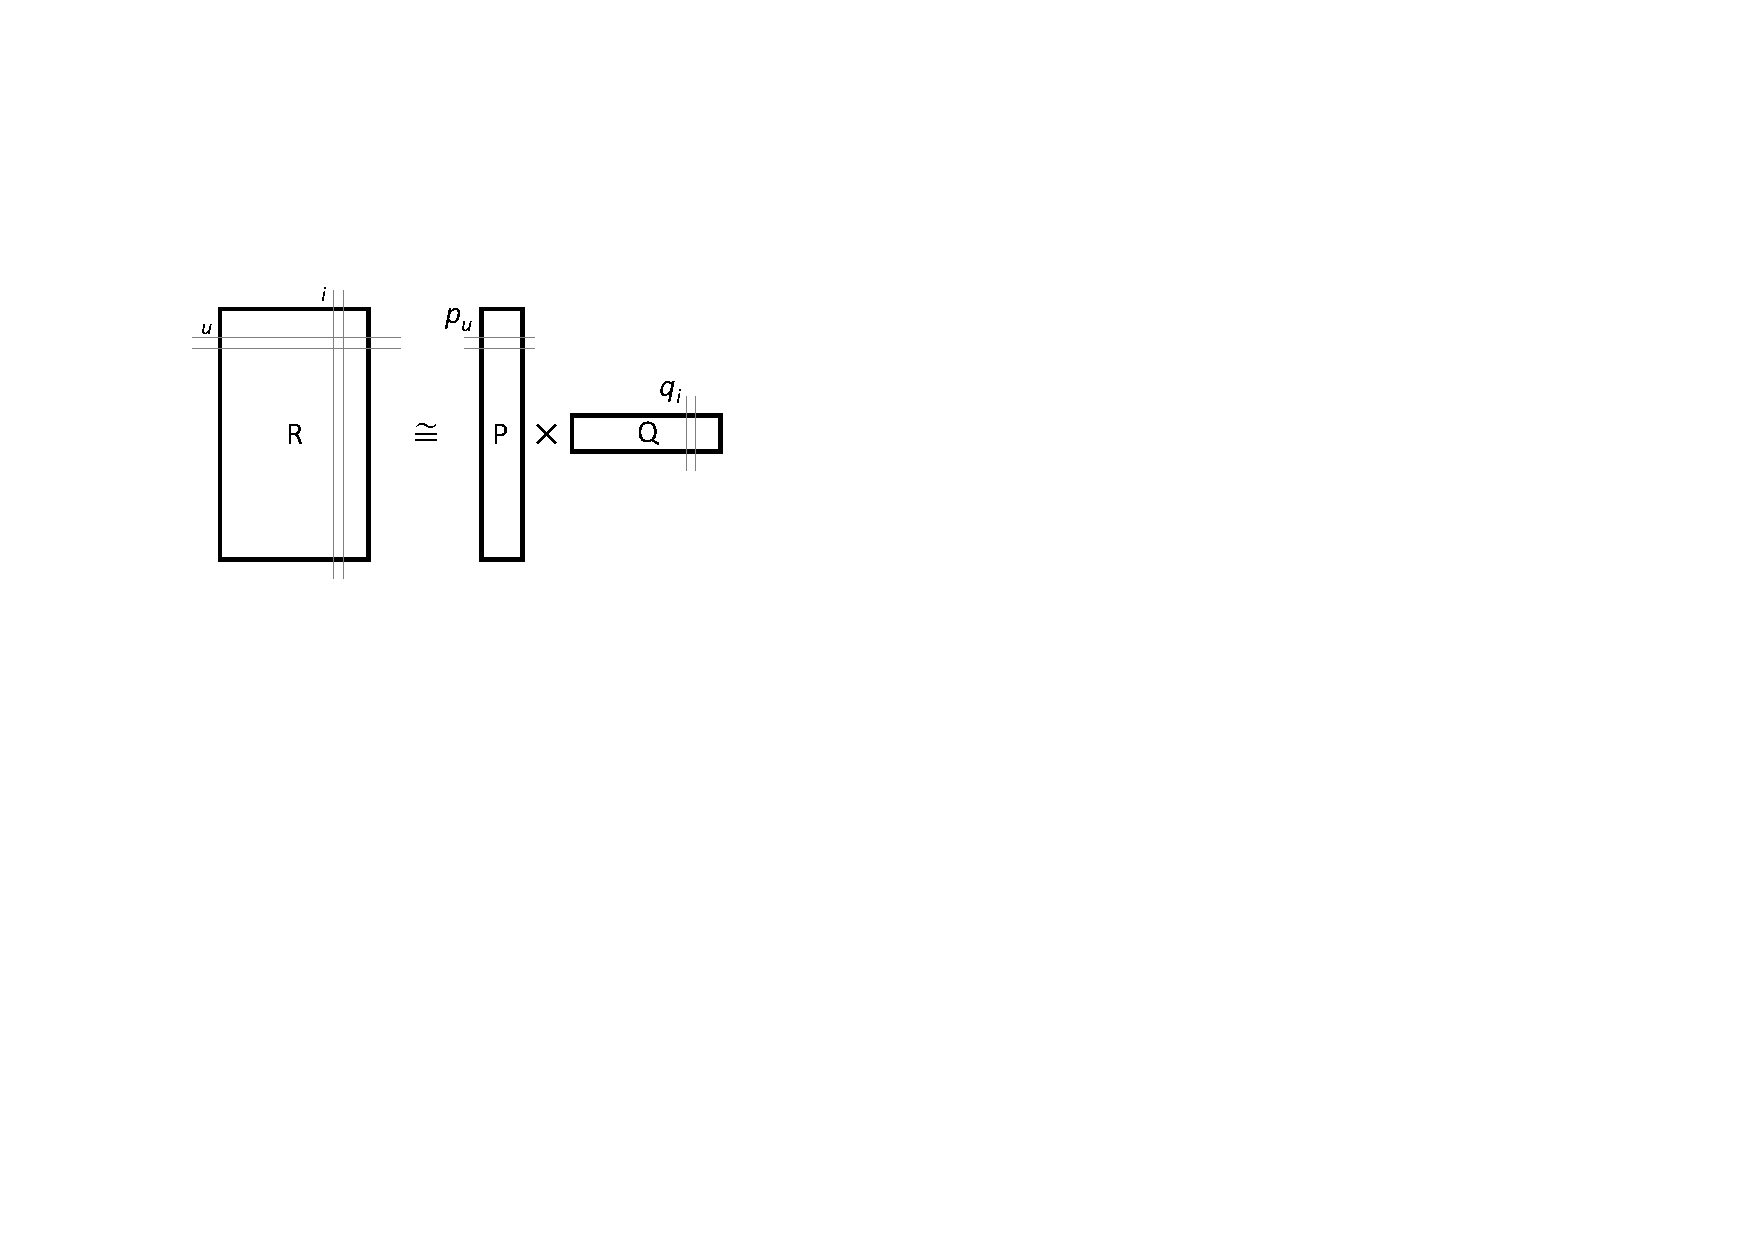
\includegraphics[width=7cm]{slike/latentni-faktorji.pdf}
\caption{Predstavitev uporabnika $u$ z latetnim profilom ${\bf p}_u$ in stvari $i$ z latentnim profilom ${\bf q}_i$. Skalarni produkt latentnih profilov nam da približek za oceno stvari $i$ uporabnika $u$, torej $\hat{r_{ui}}={\bf p}_u^T {\bf q}_i$.}
\label{f:latentni-faktorji}
\end{center}
\end{figure}

Razcep matrike R na matriki P in Q bomo poiskali tako, da bosta matriki P in Q polni, torej, da bodo vse vrednosti teh dveh matrik določene. Prav zato bomo lahko s produktom latentnih profilov lahko poiskali vrednost $\hat{r_{ui}}$ za vsako kombinacijo uporabnika $u$ in stvari $i$. Ostane nam torej le še, da izračunamo razcep, oziroma določimo matriki P in Q.

\subsection{Matrični razcep}

Z matrikami P in Q lahko izračunamo približek ocene za stvar $i$ uporabnika $u$, ki je:
%
\begin{equation}\label{eq:rui-latent}
  \hat{r_{ui}}={\bf p}_u^T {\bf q}_i = \sum_{k=1}^K p_{uk} q_{ki}
\end{equation}

Za ocene iz učne množice $r_{ui}$ bi želeli, da je ta približek čim boljši, oziroma da je napaka, ki jo s tem približkom naredimo, čim manjša. Izračunajmo kvadrat napake za oceno stvari $i$ uporabnika $u$ in ga pomnožimo z $1\over 2$, da se nam kasneje pokrajša dvojka pri odvajanju:
%
\begin{equation}\label{eq:fact-error}
  e_{ui}^2 = {1\over 2}(r_{ui}-\hat{r}_{ui})^2
\end{equation}
%
Želeli bi poiskati taki matriki $P$ in $Q$, kjer so te napake čim manjše. Ker bomo pri numeričnem iskanju teh matrik v vsaki iteraciji obravnavali natančno enega med učnimi primeri (torej $r_{ui}$ za določen par $(u,i)\in\tau$), potrebujemo izračunati gradient napake za vsakega od parametrov modela. Naš model sta matriki P in Q, vrednosti parametrov modela pa vsi njuni elementi $p_{uk}$ in $q_{ki}$. V enačbo za napako (enačba~\ref{eq:fact-error}) vstavimo izraz iz enačbe~\ref{eq:rui-latent} in odvajajmo:
%
\begin{eqnarray}
  \frac{\partial e_{ui}^2}{\partial p_{uk}} & = & -e_{ui}q_{ki} \\
  \frac{\partial e_{ui}^2}{\partial q_{ki}} & = & -e_{ui}p_{uk} \nonumber
\end{eqnarray}

Uporabimo pristop gradientnega sestopa. Matriki P in Q tokrat na začetku nastavimo na majhne naključne vrednosti. Začetna nastavitev vseh njunih elementov na 0 nas namreč ne bi pripeljala nikamor (zakaj?). Nato iteriramo po vseh elementih (trojkah) v učni množici in za vsak primer ustrezno popravimo odgovarjajoče elemente (profile) P in Q, tako da za vsak $k=1\ldots K$ popravimo vrednosti:

\begin{eqnarray}
  p_{uk} & \leftarrow & p_{uk} + \alpha e_{ui} q_{ki} \\
  q_{ki} & \leftarrow & q_{ki} + \alpha e_{ui} p_{uk} \nonumber
\end{eqnarray}

Tudi tokrat, kot pri linearni in logistični regresiji, je $\alpha$ stopnja učenja. Zgornjo enačbo lahko zapišemo tudi vektorsko:

\begin{eqnarray}
  {\bf p}_{u} & \leftarrow & {\bf p}_{u} + \alpha e_{ui} {\bf q}_{i} \\
  {\bf q}_{i} & \leftarrow & {\bf q}_{i} + \alpha e_{ui} {\bf p}_{u} \nonumber
\end{eqnarray}

Postopek iskanja razcepa matrike R na matriki P in Q, kot smo ga opisali zgoraj, imenujemo tudi inkrementalna simultana matrična faktorizacija, algoritem pa s tem dobi akronim ISMF. Gre pravzaprav za stohastični gradientni spust. Stohastični za to, ker optimizacijo vsakokrat vršimo na enem primeru iz učne množice in ne optimiziramo vrednosti P in Q za celotno učno množico hkrati.

\subsection{Regularizacija}

Zgoraj opisan matrični razcep se lahko preveč prilagodi učnim podatkom, še posebej pri večjih vrednostih $K$. Tudi tu se preveliko prileganje odrazi v velikih vrednostih parametrov modela, torej velikih vrednostih elementov matrik P in Q. Preveliko prileganje preprečimo tako, da v našo ciljno funkcijo vključimo kaznovanje, ki izhaja iz velikosti parametrov:

\begin{equation}
{e'_{ui}}^2 = {1\over 2}(e_{ui}^2 + \eta {\bf p}_u^T {\bf p}_u + \eta {\bf q}_i^T {\bf q}_i)
\end{equation}

Gradient, ki ga uporabimo pri metodi sestopa, dobimo s parcialnim odvajanjem zgornje kriterijske funkcije:
%
\begin{eqnarray}\label{e:grad-fact-reg}
  \frac{\partial {e'_{ui}}^2}{\partial p_{uk}} & = & -e_{ui}q_{ki} + \eta p_{uk} \\
  \frac{\partial {e'_{ui}}^2}{\partial q_{ki}} & = & -e_{ui}p_{uk} + \eta q_{ki} \nonumber
\end{eqnarray}
%
Upoštevaje izračunani gradient je popravek vrednosti elementov matrik P in Q v postopku gradientnega sestopa zapisan vektorsko:
%
\begin{eqnarray}\label{e:grad-descent-reg}
  {\bf p}_{u} & \leftarrow & {\bf p}_{u} + \alpha (e_{ui} {\bf q}_{i} - \eta {\bf p}_{u})\\
  {\bf q}_{i} & \leftarrow & {\bf q}_{i} + \alpha (e_{ui} {\bf p}_{u} - \eta {\bf q}_{i}) \nonumber  
\end{eqnarray}

Pri regularizaciji nastopi problem ocene primerne stopnje regularizacije $\eta$. Kot pri regresiji in klasifikaciji lahko tudi tu primerno stopnjo regularizacije ocenimo s prečnim preverjanjem in uporabimo $\eta$, pri katerem dobimo najmanjšo napako.

\subsection{Algoritem}

Elemente algoritma za matrični razcep smo pravzaprav popisali že zgoraj, a ne bo škodilo, da opišemo celotni postopek še enkrat:

\begin{tabbing}
xxx\=xxx\=xxx\=xxx \kill\\
{\bf Vhod}: učna množica $\tau'$, stopnja učenja $\alpha$, stopnja regularizacije $\eta$, stopnja razcepa $K$ \\
{\bf Izhod}: matriki P in Q \\
\\
ponastavi P in Q z naključnimi majhnimi števili ($-0.01\ldots 0.01$) \\
{\bf ponavljaj}: \\
\> {\bf za vsak} $(u,i,r_{ui})$ {\bf v} učni množici $\tau'$:\\
\>\> izračunaj $e_{ui}$\\
\>\> izračunaj gradient $e'_{ui}$ (enačba~\ref{e:grad-fact-reg})\\
\>\> {\bf za vsak} $k$ {\bf v} $1\ldots K$:\\
\>\>\> osveži $p_{uk}$ in $q_{ki}$ (enačba~\ref{e:grad-descent-reg})\\
\> {\bf končaj} ob konvergenci\\
\end{tabbing}

V zgornjem algoritmu se nam je zapisala čudna, zadnja vrstica, saj ustavitvenega kriterija nismo določili. Tudi sicer ga je težko določiti. Lahko bi postopek ustavili takrat, kadar napaka RMSE za celotno učno množico pade pod določeno mejo, ali pa kadar izvedemo več kot določeno število iteracij zgornjega algoritma (zunanja zanka), ali pa kadar se po nekaj urah naveličamo čakati, da se optimizacijskih postopek ustavi. Boljši postopek od zgornjih je, da učno množico razcepimo na dve, novo učno in validacijsko, se na novi učni naučimo, na validacijski pa preverjamo napovedi. Z učenjem prekinemo, ko se nam po na primer dveh iteracijah zunanje zanke napaka na validacijski množici ne zmanjša.

Optimizacija oziroma iskanje primernih matrik P in Q je seveda odvisna tudi od začetne nastavitve matrik. V praksi se nam obnese, da postopek nekajkrat ponovimo, vsakič z drugo inicializacijo, in upoštevamo tisti razcep, pri katerem je RMSE na učni množici, ali pa, še bolje, na validacijski množici, najmanjši.

\chapter{Povezovalna pravila}

Danes vse prodajalne, tako spletne kot te, kamor se moramo sprehoditi ali pa zapeljati z nekim prevoznim sredstvom, beležijo podatke o nakupih. Te, ki tega ne počno, so že propadle ali pa so žal na poti propada. Recimo, prodajalna prehrambenih izdelkov. Oglejmo si en zelo majhen vzorec nakupov  (tabela~\ref{t:transakcije}), kjer vsaka vrstica prikazuje, kaj je bilo v nakupovalni košarici. V tem poglavju bomo zadeve zelo poenostavili: kupci bodo ostali anonimni, čas nakupa nas ne bo zanimal, prav tako ne bomo beležili števila nakupljenih stvari. Zanimali nas bodo samo tipi nakupljenih stvari v nakupovalnih košaricah (na primer, mleko, ne pa tri litre mleka, in ne pol štruce kruha).

\begin{table}
\caption{Podatki o nakupovalnih košaricah.}
\label{t:transakcije}
\begin{center}
\small
\begin{tabular}{lll}
\toprule
nakup & stvari v košarici & poenostavljen zapis \\
\midrule
$t_1$ & mleko, kruh & MK \\
$t_2$ & mleko, sir, zelenjava & MSZ \\
$t_3$ & kruh, sir, zelenjava & KSZ \\
$t_4$ & mleko, kruh, sir, zelenjava & MKSZ \\
$t_5$ & mleko, kruh, sir & MKS \\
$t_6$ & kruh, sir & KS \\
$t_7$ & sir & S \\
$t_8$ & kruh, zelenjava, sir & KZS \\
$t_9$ & sir, zelenjava & SZ \\
$t_{10}$ & kruh, sir, zelenjava & KSZ \\
\bottomrule
\end{tabular}
\end{center}
\end{table}

Nakupovalne košarice smo označili s $t_i$ za $i$-to nakupovalno košarico. Bolj strokovno vsaki vrstici v tabeli~\ref{t:transakcije} pravimo tudi {\em transakcija}. Naj bo množica transakcij, katero bi želeli preučiti, ${\mathcal T}=\{t_1,t_2,\ldots t_N\}$. Množico stvari, ki lahko nastopajo v teh transakcijah, označimo z ${\mathcal I}=\{i_1,i_2,\ldots i_M\}$.

\section{Nabori in podnabori}

Terkam stvari, kot so na primer \{kruh, sir\} ali pa \{mleko, sir, zelenjava\} pravimo {\em nabor}. Za par naborov $X$ in $Y$ pravimo, da je $X$ podnabor nabora $Y$, če je vsaka stvar iz nabora $X$ vsebovana v naboru $Y$. V tem primeru zapišemo, da velja $X\subseteq Y$. Nabor \{kruh, sir\} je na primer podnabor nabora \{kruh, mleko, sir\}. Števnost stvari v naboru $X$ označimo $|X|$. V naboru $X=\{{\rm kruh}, {\rm mleko}, {\rm sir}\}$ so tri stvari, $|X|=3$. Nabor $X$ s števnostjo $|X|$ ima $2^{|X|}$ možnih podnaborov, med katerimi je tudi prazen podnabor $\emptyset$.

\section{Podpora in pogosti nabori}

S $\sigma(X)$ označimo število transakcij, ki vsebuje podnabor $X$. Podnabor $X=\{{\rm mleko}, {\rm kruh}\}$ je vsebovan v transakcijah $t_1$, $t_4$ in $t_5$. Število podprtih transakcij za nabor $X$ je zato enako tri, oziroma $\sigma(X)=3$. Število $\sigma(X)$ formalno določimo s sledečim zapisom:
%
\begin{equation}
  \sigma(X)=|\{t_i|X\subseteq t_i, t_i\in {\mathcal T}\}|
\end{equation}

Iz števila podprtih transakcij za nabor $X$ lahko izračunamo delež podprtih transakcij, torej delež transakcij, ki vsebujejo nabor $X$:
%
\begin{equation}
  s(X)={\sigma(X)\over |{\mathcal T}|}={\sigma(X)\over N}
\end{equation}

Zanima nas, kateri nabori so taki da za njih velja
\begin{equation}
  s(X)\geq{\rm minsupp}
\end{equation}
kjer je ${\rm minsupp}$ minimalna podpora oziroma parameter, ki ga določi uporabnik. Nabore, kjer velja zgornji izraz, imenujemo {\em pogosti nabori}.

\section{Algoritem Apriori}

Za iskanje vseh pogostih naborov v množici transakcij bomo razvili algoritem Apriori, ki sta ga sicer predlagala Agrawal in Srikant leta 1994. A preden zapišemo algoritem, razmislimo o nekaj lastnostih prostora vseh možnih naborov. Ti so za naš primer grafično prikazani v mreži naborov (slika~\ref{f:mreza-naborov}), kjer so nabori določenega nivoja povezani z nabori prejšnjega nivoja, če so slednji njihovi podnabori. Tako je vozlišče MKZ povezano z vozlišči MK, MZ in KZ, a ne z vozliščem MS, saj MS ni podnabor MKZ.

\begin{figure}[htbp]
\centering{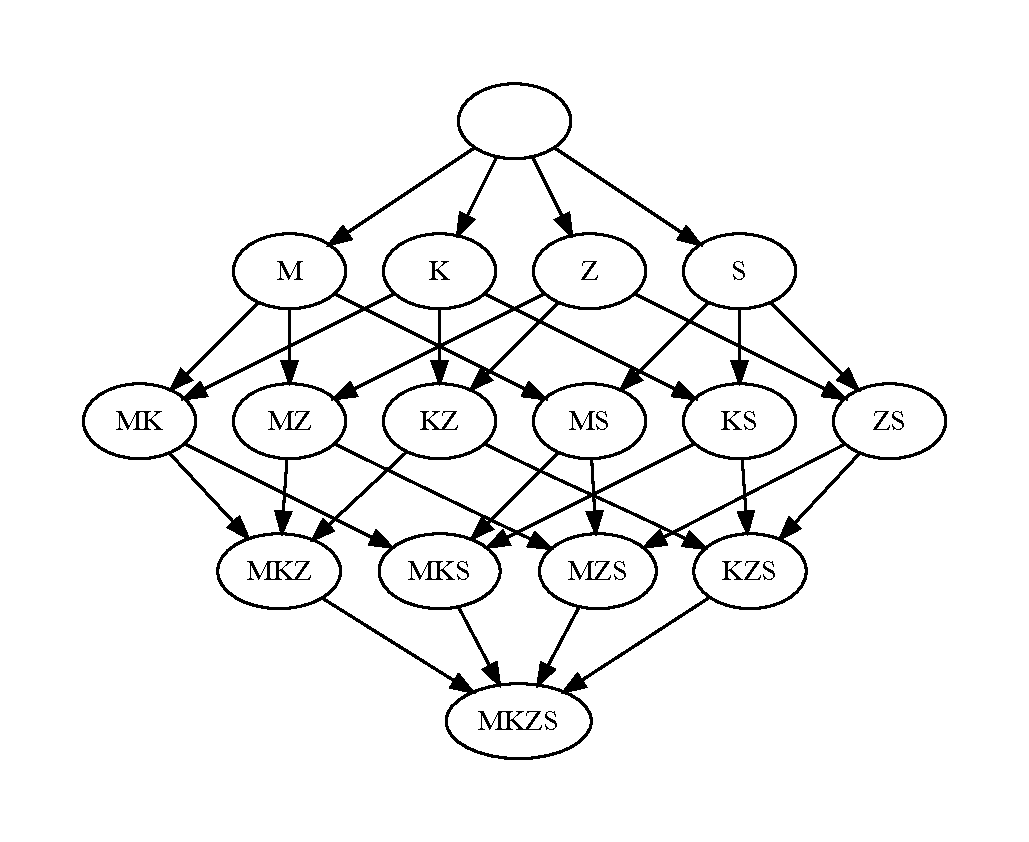
\includegraphics[width=9cm]{slike/mreza-naborov.pdf}}
\caption{Mreža vseh možnih naborov za množico stvari mleko (M), kruh (K), zelenjava (Z) in sir (S). V korenu grafa je prazen nabor.}
\label{f:mreza-naborov}
\end{figure}

Recimo, da iščemo pogoste nabore s podporo vsaj 0.6 (${\rm minsupp}=0.6$). Najprej za vsak nabor v mreži naborov določimo število transakcij, v katerih je ta nabor prisoten. Za naš primer tako označeno mrežo prikazuje slika~\ref{f:mreza-pogostih-naborov}. Pogosti nabori morajo biti vsebovani vsaj v šestih transakcijah. Iz mreže je razvidno, da to velja za šest naborov, med katerimi je eden prazen.

Iz mreže naborov lahko razberemo nekaj zanimivih zakonitosti. Recimo, nabor M je nepogost. Zaradi tega so nepogosti prav vsi nabori z mlekom, torej vsi nabori, katerih podnabor je M. To je razumljivo, saj vsi ti nabori zahtevajo, da je njhov podnabor tudi M, ta pa je vsebovan v pramajhnem številu transakcij, da bi bili nabori, ki ga vsebujejo, pogosti.

Prav tako razberemo, da podpora nabora ne more presegati podpore kateregakoli njegovega podnabora. Primer: KZS je vsebovan v štirih transakcijah, in to število ne sme presegati števila transakcij, v katerih so vsebovani vsi njegovi možni podnabori, torej tudi ti iz prejšnjega nivoja (KZ, KS, ZS).

\begin{figure}[htbp]
\centering{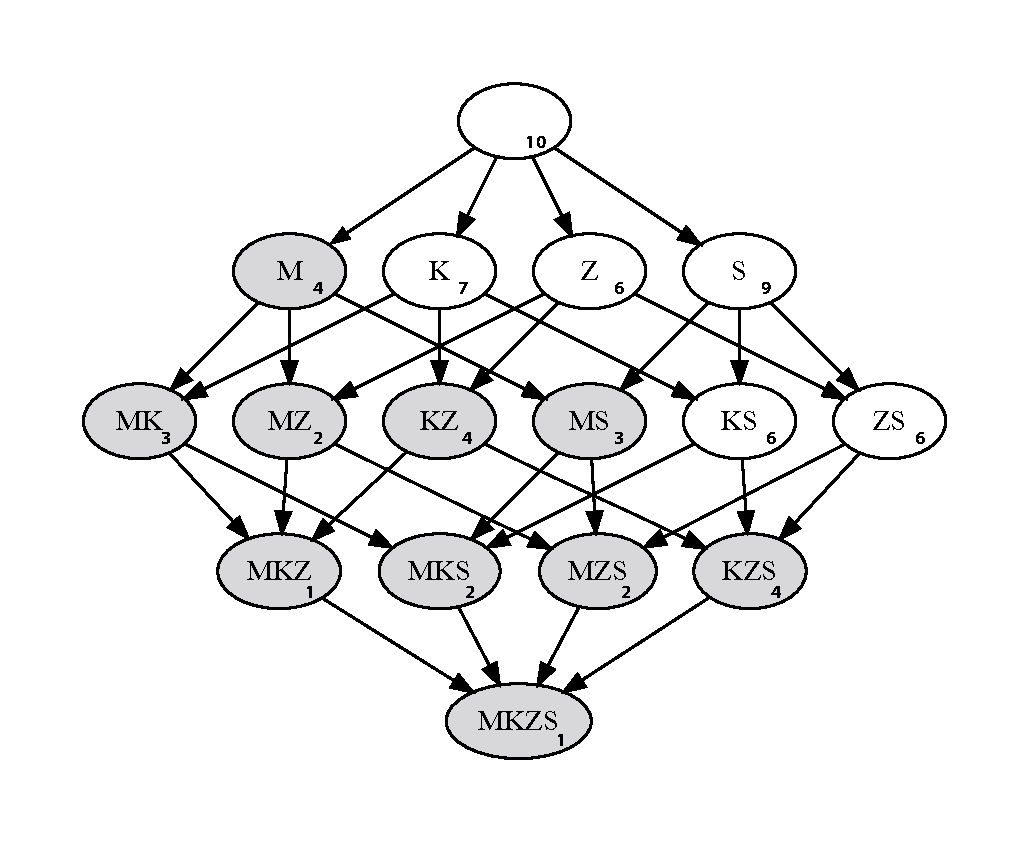
\includegraphics[width=9cm]{slike/mreza-pogostih-naborov.pdf}}
\caption{Mreža pogostih naborov (naborov v praznih vozliščih) za ${\rm minsupp}=0.6$ oziroma za vse nabore, katerih število podpornih transakcij je vsaj 6 ($6=0.6\times 10$). Vozlišča, ki predstavljajo nepogoste nabore, so osenčena.}
\label{f:mreza-pogostih-naborov}
\end{figure}

Zgornja zapažanja zapišimo v obliki teoremov.

\begin{teorem}
  Če je nabor pogost, so pogoste tudi vse njegove podmnožice:
  $$s(X)\geq{\rm minsupp}\implies s(Y)\geq{\rm minsupp}, Y\subseteq X$$
\end{teorem}

\begin{teorem}
  Če je nabor nepogost, so nepogosti tudi vsi nabori, ki ga vsebujejo:
  $$s(X)<{\rm minsupp}\implies s(Y)<{\rm minsupp}, X\subseteq Y$$
\end{teorem}

\begin{teorem}
  Podpora nabora nikoli ne presega podpore njegove podmnožnice (antimonotonost, ${\mathcal L}=2^I$ je močnostna množica, torej množica vseh možnih naborov):
  $$ \forall X,Y\in {\mathcal L}: X\subseteq Y\implies s(Y)\leq s(X) $$
\end{teorem}

Iz zgornjega intuitivno sledi algoritem Apriori. Ker nas prazna množica ne zanima, pričnemo lahko s pogostimi nabori prvega nivoja, torej nabori, ki vsebujejo natanko eno stvar (te imenujemo tudi {\em pogosti 1-nabori}). Od tu dalje s kombinacijo pogostih naborov generiramo {\em pogoste $k$-nabore}, kjer $k$ iterativno povečujemo. Ustavimo se, ko na $k$-tem nivoju ni več pogostih naborov, saj bi to pomenilo, da teh tudi ni v vseh višjih nivojih.

\begin{tabbing}
xxx\=xxx\=xxx\=xxx \kill\\
{\bf Vhod}: množica transakcij in minimalna podpora minsupp \\
{\bf Izhod}: množica pogostih naborov \\
\\
$k=1$ \\
$F_k=\{i|i\in I\land\sigma(i)\geq N\times{\rm minsupp}\}$ \\
{\bf ponavljaj} \\
\> $k\leftarrow k+1$ \\
\> $C_k={\rm kandidati}(F_{k-1})$ \\
\> izračunaj podporo naborov v $C_k$ \\
\> $F_k=\{c | c\in C_k\land\sigma(c)\geq N\times{\rm minsupp}\}$ \\
{\bf dokler} $F_k=\emptyset$ \\
{\bf vrni} $\cup_k F_k$ \\
\end{tabbing}

Algoritem Apriori uporablja funkcijo kandidati, ki na podlagi že odkritih pogostih naborov tvori pogoste $k$-nabore. S podrobnostmi implementacije te funkcije se ne bomo ukvarjali, omenimo pa samo, da so za hitrost celotnega algoritma precej pomembne. Namreč, izogniti se moramo tvorjenju enakih kandidatov. Recimo, nabor KS lahko tvorimo iz pogostega nabora K in stvari S, ali iz pogostega nabora S in stvari K. Tu omenimo samo nekaj možnosti, ki jih lahko pri tvorjenju kandidatov lahko uporabimo:
\begin{itemize}
\item Kandidate za $F_k$ tvorimo iz kombinacije pogostih naborov $F_{k-1}\times F_1$. Problem podvojenih kandidatov rešimo z leksikografsko ureditvijo naborov (na primer MKZ je z MZS, saj je K leksikografsko pred Z).
\item Kandidate za $F_k$ tvorimo iz kombinacije pogostih naborov $F_{k-1}\times F_1$, kjer nabora združimo le, če sta različna samo v zadnjem elementu. Tudi tu problem podvojenih kandidatov rešujemo z leksikografsko ureditvijo naborov.
\end{itemize}

\section{Povezovalna pravila}

Pravila tipa
$$ X\rightarrow Y $$
kjer sta X in Y nabora stvari, imenujemo {\em povezovalna pravilna}. Zahtevamo, da je presečna množica obeh naborov prazna, torej $X\cap Y=\emptyset$. Primer takega pravila je recimo
$$ {\rm kruh}\to {\rm mleko}, {\rm sir}$$
pravilo pa pravi, da če bo v košarici kruh, pričakujemo, da bosta tam tudi mleko in sir. Še en primer povezovalnega pravila je
$$ {\rm mleko}, {\rm sir}\to {\rm zelenjava} $$
ki pravi, da če bo v košarici mleko, pričakujemo, da bosta tam tudi sir in zelenjava.

Pravila so lahko seveda bolj ali manj v soglasju z učno množico transakcij. Povezovalna pravila ocenjujemo z merami, med katerima sta najbolj znani podpora in zaupanje. {\em Podporo} že poznamo, poroča pa o delež transakcij, kjer najdemo vse stvari iz povezovalnega pravila:
\begin{equation}
  s(X\to Y)={\sigma(X\cup Y)\over N}
\end{equation}
Podpora torej meri pogostost pravila v množici transakcij.

Drugačna mera je {\em zaupanje}, ki meri, kakšen je delež transakcij, ki vsebujejo desno stran pravila $Y$ med transakcijami, ki vsebujejo levo stran pravila $X$:
\begin{equation}
  c(X\to Y)={\sigma(X\cup Y)\over\sigma(X)}
\end{equation}

Za pravilo ${\rm M}\to {\rm SK}$ bo tako podpora enaka $0.2$, zaupanje pa enako $0.5$ (štiri transakcije vsebujejo mleko, od tega dve poleg mleka še sir in kruh). Podpora pravila ${\rm Z}\to{\rm S}$ bo $0.6$, zaupanje pa $1.0$.

Algoritmu za iskanje podpornih pravil predpišemo ${\rm minsupp}$ in ${\rm minconf}$, torej minimalno podporo in minimalno zaupanje. V praksi pa pravila iščemo tako, da najprej poiščemo pogoste nabore, potem pa iz teh izluščimo pravila, katerih zaupanje je dovolj visoko. Pogosti nabori bodo namreč imeli enako podporo kot pravila, ki vsebujejo vse stvari iz pogostega nabora. Iz nabora ${\rm KZS}$ lahko tako tvorimo $2^3-2=6$ netrivialnih pravil, kjer je leva oziroma desna stran pravila neprazna:

\begin{center}
  KZ$\to$S, KS$\to$Z, ZS$\to$K, \\
  S$\to$KZ, Z$\to$KS, K$\to$ZS
\end{center}

Za dani nabor stvari lahko tvorimo vsa možna povezovalna pravila na podoben način, kot smo tvorili vse možne podnabore. Z eno samo razliko. Tokrat podnabore v mreži uporabimo za desno stran povezovalnega pravila, na levo stran pa damo vse, kar je v naboru, ki ga cepimo v pravilo, še ostalo. Tako nam za nabor ${\rm KZS}$ mreža na sliki~\ref{f:pravila-kzs} podaja vse možne cepitve oziroma vsa možna pravila.

\begin{figure}[htbp]
\centering{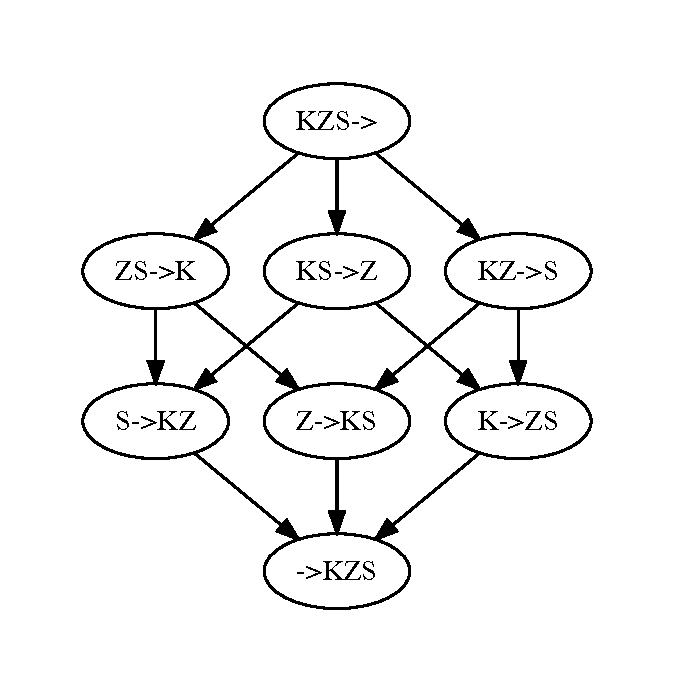
\includegraphics[width=9cm]{slike/pravila-kzs.pdf}}
\caption{Mreža vseh možnih povezovalnih pravil, ki jih lahko tvorimo iz nabora KZS. Pravili v korenu (prazen nabor na levi strani) in na zadnjem nivoju mreže nista legalni, sta pa vseeno prikazani.}
\label{f:pravila-kzs}
\end{figure}

Ostane nam le, da tudi tu poiščemo finto oziroma pristop, kjer je mrežo povezovalnih pravil graditi iz začetnega vozlišča tako, da kandidate klestimo glede na zahtevano zaupanje. V ta namen si oglejmo dve pravili, ki ju tvorimo iz nabora Z: ${\rm X}\to {\rm Z}-{\rm X}$ in ${\rm X'}\to {\rm Z}-{\rm X}'$. Vsakič smo torej desno stran pravila dobili tako, da smo od nabora ${\rm Z}$ odstranili stvari na levi strani pravila, ki so enkrat bile X in drugič ${\rm X}'$.

\begin{teorem}
  Naj bosta ${\rm X}$ in ${\rm X}'$, kjer je ${\rm X}'$ podnabor {\rm X}. Velja:
  $$c({\rm X}\to {\rm Z}-{\rm X})<{\rm minconf}\implies c({\rm X}'\to {\rm Z}-{\rm X}')<{\rm minconf} $$
\end{teorem}
Ta teorem moramo dokazati. Spomnimo se, da velja:
$$ {\rm X}'\subset {\rm X}\implies\sigma({\rm X}')\geq\sigma({\rm X}) $$
Neenačbo na desni strani pomnožimo z $\sigma(Z)$ in delimo z $\sigma({\rm X}')$ ter $\sigma({\rm X})$. Dobimo enačbi za zaupanje obeh pravil, in dokaz zgornjega teorema:
$${\sigma({\rm Z})\over\sigma({\rm X}')} < {\sigma({\rm Z})\over\sigma({\rm X})}$$

Z drugimi besedami: če ${\rm X}\to Z-X$ ne presega minimalnega zaupanja, tudi ${\rm X'}\to {\rm Z}-{\rm X}'$ ne bo, kjer je ${\rm X}'$ podnabor ${\rm X}$. V naši mreži povezovalnih pravil s slike~\ref{f:pravila-kzs} vidimo, da so pravila s podnabori levih strani postavljena v spodnjih nivojih pravil nivoja nad njimi. Če pravilo ZS$\to$K ne bo ustrezalo pogoju zaupanja, tudi pravili S$\to$KZ in Z$\to$KS, ki iz njega sledita, ne bodo.

Ravno smo torej ``izumili'' pristop gradnje povezovalnih pravil. Gradimo jih iz pogostega nabora. Uporabimo mrežo pravil, kjer pričnemo s prazno desno stranjo pravila in tej, na vsakem nivoju, dodamo po eno stvar ter na ta način tvorimo vse možne kombinacije. Pravila na nivoju $k$ gradimo s kombinacijo pravil nivoja $k-1$. Kot pri algoritmu Apriori tudi tu na vsakem nivoju hranimo samo pravila, ki ustrezajo kriteriju zaupanja.

Za velike množice transakcij gradnja povezovalnih pravil kaj lahko privede do nepreglednih množic pravil. To se seveda zgodi pri premalo ostrih pogojih, torej pri premalo visokih minsupp in minconf. Taka pravila je ročno nemogoče pregledati. Pomagamo si tako, da skušamo najprej zmanjšati množico pogostih naborov z dvigovanjem minsupp, potem pa iz nje tvorimo pravila tako, da najprej skušamo postavljati bolj ostre pogoje za zaupanje. 

% \chapter{Projekcije podatkov}

Ena od težav, na katero naletimo pri uporabi hierarhičnega razvrščanja v skupine, je, da lahko napačno sugerira, da so si vsi predstavniki določene skupine med seboj podobni bolj, kot so podobni članom drugih skupin. Hierarhija skupin tako lahko daje uporabno in smiselno sliko podatkov, obenem pa je rigidna in ne dopušča "mehkega" članstva v skupinah.

Primer kaže slika~\ref{f-jeziki-hclust}. Angleščina je germanski jezik, ki se je razvijal pod vplivom romanskih, predvsem francoščine. Hierarhično gručenje jo mora nekam uvrstiti in dalo jo je k romanskim, čeprav bi jo pravzaprav lahko tudi k germanskim; če tega ne bi vedeli, bi iz gručenja sklepali, da je angleščina romanski jezik. Podobne težave ima italijanščina: je res podobnejša francoščini kot španščini? Morda ne. Postopek gručenja je najprej združil španščino in portugalščino; italijanščina je sicer morda blizu španščini, a tako različna od portugalščine, da je podobnost med italijanščino in francoščino večja kot med italijanščino in skupino španščina-portugalščina.

\begin{figure}[b!]
\begin{center}
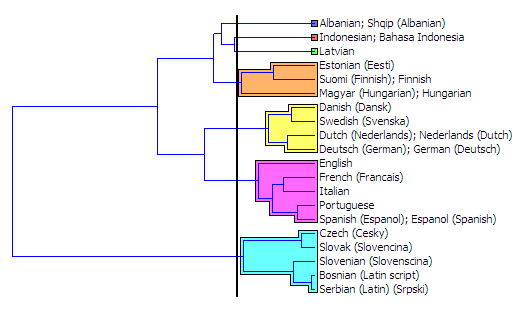
\includegraphics[width=12cm]{slike/jeziki-clustering.png}
\caption{Hierarhične gruče jezikov na podlagi podobnosti besed v prevodu Deklaracije o človekovih pravicah}
\label{f-jeziki-hclust}
\end{center}
\end{figure}

Razvrščanje v skupine je vseeno odličen postopek, ki ga bomo uporabili pač takrat, kadar želimo razvrstiti primere, na primer jezike, v skupine. Kadar pa si bolj želimo ustvariti podobo o podatkih, pa uporabimo katero od tehnik za projeciranje podatkov iz višjih v nižje -- recimo dvo- -- dimenzionalne prostore.

Med najbolj znanimi je večrazsežnostno lestvičenje ({\em multidimensional scaling}, MDS), ki iz matrike razdalj med objekti sestavi dvodimenzionalni zemljevid primerov, v katerih se razdalje čim bolj ujemajo z želenimi.

Nekoliko podobna tehnika je FreeViz. Za delovanje potrebuje seznam primerov v podobni obliki kot pri atributnem učenju: vsak primer je opisan z vrednostmi atributov in razredom. FreeViz poišče projekcijo v dve dimenziji, v katerih so primeri iz istega razreda čim bližje, primeri iz različnih razredov pa čim dalj eden od drugega.

Tretji postopek za projekcijo primerov v nižje-dimenzionalen prostor, ki ga bomo opisali, je analiza osnovnih komponent ({\em principle components analysis}, PCA). PCA je prav gotovo najbolj znana metoda za iskanje informativnih projekcij za množico podatkov. PCA  predpostavi, da se podatki, ki so sicer opisani z večjo množico atributov, v resnici nahajajo v nižjedimenzionalnem prostoru. PCA poišče osnovne komponente, to je, smeri, ki "napenjajo" množico primerov. Podobna metoda je faktorska analiza, obenem pa je PCA podoben tudi drugim oblikam dekompozicije, kot je, na primer, SVD. PCA se tipično ne uporablja za vizualizacijo podatkov, temveč predvsem za predstavitev podatkov z manjšo, razumljivejšo in zanesljivejšo množico atributov.

\section{Večrazsežnostno lestvičenje (MDS)}

Denimo, da trije Marsovčki ne bi prišli k Drejčku, temveč bi se z njim pogovarjali le po mobitelu. Radovedni Marsovčki bi radi izvedeli kaj o Sloveniji; ko bi jim Drejček tako našteval različne kraje in njihove znamenitosti, bi si Marsovčki počasi zaželeli malo več predstave o tem, kaj je kje. Drejček ima pri sebi zemljevid. Koordinatnega sistema še ne pozna, pač pa je ob zemljevidu tabela razdalj med vsemi pari (večjih) krajev. Je mogoče iz teh podatkov rekonstruirati zemljevid?

Seveda je. Drejček jim zrecitira tabelo in Marsovčkom je storiti naslednje: najprej vzamejo tri kraje, recimo Maribor, Kranj in Ljubljano, ter jih narišejo v trikotnik s podanimi razdaljami (v določenem merilu). Nato jemljejo vse ostale kraje, enega za drugim, in jih razpostavljajo na ustrezne razdalje od teh treh. Se lahko to kje zalomi? Prvo, kar bo šlo očitno vedno narobe, vendar nas sploh ne moti, je, da bo zemljevid obrnjen bogvekako, pa še prezrcaljen zna biti. Nič hudega, ne le Marsovčki, že Avstralci bi videli Slovenijo prezrcaljeno, če bi bila Zemlja steklena. Druga težava, do katere pri risanju Slovenije ne bo prišlo, pri risanju drugih reči pa, so nemogoče razdalje. Recimo, da bi Drejček Marsovčkom sporočil, da je od Ljubljane do Celja 65 kilometrov, od Celja do Maribora tudi 65, od Ljubljane do Maribora pa 150 km. V tem primeru, bodo rekli Marsovčki, si se, dragi Drejček, očitno zmotil: tega ni mogoče narisati, saj trikotnika s stranicami 65, 65 in 150 ni.

Idejo risanja zemljevidov iz podatkov lahko uporabimo tudi za podatke, ki v resnici niso prostorski. Tako lahko, recimo, narišemo zemljevid jezikov (Slika~\ref{f-jeziki-mds}), pri čemer so razdalje, tako kot pri gručenju, definirane na podlagi podobnih besed, ki se pojavljajo v prevodu Deklaracije o človekovih pravicah. Da bi bila slika preglednejša, smo na njej povezali 10\% najbolj podobnih parov jezikov. Slika lepo razpade na slovansko, romansko in germansko skupino, pri čemer je angleščina nekoliko na svojem (a še vedno bolj povezana z romanskimi kot germanskimi jeziki). Obenem je očitno tudi, da so si germanski in romanski jeziki med seboj podobni (zgodovinsko gledano je to najbrž posledica dejstva, da so se romanski jeziki razvijali iz latinščine pod vplivom prišlekov s severa), slovanski pa so nekje posebej.

\begin{figure}[tbp]
\begin{center}
\includegraphics[width=12cm]{slike/jeziki-mds.png}
\caption{Zemljevid jezikov, dobljen z večrazsežnostnim lestvičenjem; razdalje so definirane na podlagi besed v prevodu Deklaracije o človekovih pravicah}
\label{f-jeziki-mds}
\end{center}
\end{figure}


Prvega Drejčkovega problema tu ni: govoriti o tem, da je zemljevid jezikov obrnjen narobe, je nesmiselno, saj se jeziki v resnici ne nahajajo v prostoru. Pač pa imamo -- odvisno od tega, na kakšen način je definirana razdalja -- tu morda drugi problem: zemljevida, v katerem bi razdalje natančno odgovarjale želenim (v določenem merilu, seveda), morda sploh ni mogoče narisati, saj takšna postavitev ne obstaja. Nič ne de: namesto ``točnega'' zemljevida, bomo zadovoljni tudi s približnim. 

Kako ga narisati? Takole: objekte si predstavljajmo kot kroglice, ki jih povežemo z vzmetmi, katerih dolžine ustrezajo želenim razdaljam (predstavljajmo si, da gre za posebne vzmeti, ki se ne zavozljajo temveč lahko prehajajo ena skozi drugo). Dobimo veliko žogo iz krogel in vzmeti, a ko jo izpustimo fizika opravi svoje -- krogle se razletijo in razmestijo tako, da so vse vzmeti karseda ``sproščene'', ne predolge in ne prekratke.

Računalniško izvedbo tega algoritma imenujemo večrazsežnostno lestvičenje ({\em multidimensional scaling}, MDS). Formalno ga zastavimo tako, da definiramo energijo sistema ali napetost ({\em stress}) kot, recimo,
$$\sigma(\mathbf{X}) = \sum_{i\ne j} (d_{ij} - \delta_{ij})^2,$$
kjer je $\mathbf{X}$ trenutni razpored točk, $d_{ij}$ in $\delta_{ij}$ pa trenutna in želena razdalja med točkama $i$ in $j$. Večrazsežnostno lestvičenje poišče razpored $\mathbf{X}$ z najmanjšo napetostjo $\sigma(\mathbf{X})$.

Kako minimizirati takšno funkcijo? Analitično ne bo šlo. Za to bi bilo potrebno odvesti $\sigma(\mathbf{X})$ po vseh koordinatah ($x_i$ in $y_i$) in poiskati ničle. Razdalja med točkama $i$ in $j$ je enaka $d_{ij}=\sqrt{(x_i-x_j)^2+(y_i-y_j)^2}$, torej bo
\begin{eqnarray*}\frac{\partial\sigma({\mathbf{X}})}{\partial x_i} & = &
\sum_{j\ne i} \frac{\partial\sigma({\mathbf{X}})}{\partial d_{ij}}\frac{d_{ij}}{\partial x_i} \\ & =
& \sum_{j\ne i} -2\left(\delta_{ij}-\sqrt{(x_i-x_j)^2+(y_i-y_j)^2}\right) \frac{(x_i-x_j)}{\sqrt{(x_i-x_j)^2+(y_i-y_j)^2}}
\end{eqnarray*}
Pri stotih točkah bi dobili sistem z dvesto takšnimi enačbami; ideji o direktnem napadu se torej raje odpovemo.

Drug, izvedljiv postopek je gradientna metoda: izračunamo gradient funkcije $\sigma(\mathbf{X})$, se pravi odvod po vseh spremenljivkah. To smo pravzaprav storili že zgoraj. Izberemo si poljuben začetni razpored točk, vstavimo koordinate v odvode, dobimo gradient (vektor odvodov) in se pomaknemo v smeri nasprotni gradientu, se pravi, vse točke pomaknemo v smer, kamor jih potiskajo odvodi. Kot vemo iz analize ali od kod drugod, nas bo to počasi pripeljalo v minimum. (Takšen algoritem počne natančno to, kar bi počela narava z vzmetmi: odvod energije po položaju je sila, torej gradientna metoda pomika vse točke v smeri sile.)

Gradientna metoda bi delovala, vendar ne prav dobro. Bila bi počasna in velikokrat bi nas (lahko) pripeljala le v lokalni minimum. V fizikalni metafori, krogle in vzmeti bi se znašle v neki lokalno stabilni konfiguraciji, vendar bi jih bilo mogoče ``potisniti'', preobrniti tako, da bi se ``zoptimizirale'' tudi v kaj boljšega.

V svetu optimizacijskih problemov je gradientna metoda le metoda grobe sile, ki jo bomo uporabili, če se ne moremo spomniti ničesar boljšega. Eden od boljših postopkov je ``majorizacija''. Označimo funkcijo, katere minimum iščemo, z $f(x)$. Recimo, da si znamo izmisliti, neko drugo funkcijo $g(x, y)$, ki je stalno večja ali enaka $f(x)$ (torej, za vsak $y$ velja $g(x, y)\ge f(x)$ pri vsakem $x$), v točki $g(x, x)$ pa velja $g(x, x)=f(x)$. Funkcija $g(x, y)$ naj bo takšna, da znamo dobro poiskati vrednost $x$, pri katere doseže minimum. Zdaj lahko počnemo tole: izmislimo si začetni $x_0$. Pri njem, vemo, velja $g(x_0, x_0)=f(x_0)$. Minimiziramo funkcijo $g$ in dobimo nov, boljši $x$ - označimo ga z $x_1$. Vrednost $g(x_1, x_0)$ je manjša ali enaka vrednosti $g(x_0, x_0)$, saj smo minimizirali $g$ po prvem argumentu. Po drugi strani, spet po definiciji funkcije $g$, velja $f(x_1) \le g(x_1, x_0)$. Imamo torej
$$f(x_1) \le g(x_1, x_0) \le g(x_0, x_0) = f(x_0)$$
Postopek ponovimo z $x_1$, da pridelamo naslednji, še boljši $x_2$.

Takšna optimizacija je, tako kot gradientna metoda še vedno iterativna, vendar hitrejša. Koliko hitrejša, je odvisno od tega, kako dobro $g(x, y)$ smo poiskali; $g(x, y)$ se mora čim tesneje prilegati $f(x)$, poleg tega pa jo moramo biti zmožni čim boljše optimizirati.

Algoritem večdimenzionalnega lestvičenja, ki deluje na ta način, se imenuje SMACOF ({\em Scaling by majorizing a complicated function}). SMACOF je hitrejši od gradientne metode, dela večje korake in se manjkrat zatakne v lokalnih ekstremih, zato je uporabnejši za (realistične) primere, v katerih je točk veliko.

Za izračun napetosti lahko namesto gornje, naivne formule uporabljamo tudi takšne, ki uteži prispevke parov (predpišemo lahko, za katere pare si še posebej želimo, da bi razdalja ustrezala pravi), poleg tega pa lahko napetost posameznega para normiramo tako, da jo delimo z želeno ali s trenutno razdaljo.

Slika~\ref{f-zoo-mds} kaže zemljevid živali. Razdalje med pari živali so izračunane kot evklidske razdalje med atributi, ki jih opisujejo. Točke, ki predstavljajo živali, smo obarvali glede na vrsto -- vijolični so sesalci, rdeče ptice, oranžno žuželke. Povezani so pari živali, ki so si med seboj najbolj podobne.

\begin{figure}[tbp]
\begin{center}
\includegraphics{slike/zoo-mds.pdf}
\caption{Zemljevid živali (podatkovna zbirka Zoo)}
\label{f-zoo-mds}
\end{center}
\end{figure}

Čeprav MDS ni uporabljal podatkov o vrstah živali, so različne vrste na zemljevidu dobro ločene. Vidimo tudi nekaj podobnosti med živalmi: morske sesalce je MDS postavil v bližino rib; dvoživke so blizu rib in nevretenčarjev, predvsem morskih; žuželke so pomešane s ptiči.

Vidimo tudi težavo: žuželke so razdeljene v dve skupini. MDS se je očitno znašel v lokalnem ekstremu, saj bi morale ose in čebele k ostalim žuželkam, vendar bi jih moral optimizacijski postopek peljati okrog ptičev. To se zgodi kar pogosto in pomagamo si tako, da podatke nekoliko potresemo, naključno premaknemo točke, ali pa začnemo celotno optimizacijo znova.

Večrazežnostno lestvičenje je torej postopek, ki vizualizira podatke v obliki zemljevida. Podatki so opisani s seznamom primerov in razdalj med njimi; lastnosti primerov niso potrebne in jih ne znamo upoštevati (razen, če iz le-teh računamo razdalje, kot smo storili pri živalih). Zemljevid je nezanesljiv v tem smislu, da bodo različne naključne začetne postavitve vodile v različne končne slike, a vsaka od njih nam lahko nudi drugačen pogled na podatke. Prav tako je nezanesljiv položaj posameznih točk; dogaja se, da je točka obtičala v lokalnem minimumu, čeprav v resnici ne sodi na to mesto. Takšne točke lahko prepoznamo, če zemljevidu dodamo povezave med najbolj podobnimi pari. Obenem nam takšne povezave pomagajo brati sliko. MDS ne sestavlja gruč, pač pa lahko gruče razberemo sami.


\section{FreeViz}

Denimo, da imamo primere, ki so opisani z atributi, za vsak primer pa je podan tudi razred. Zemljevid takšnih podatkov bi sicer lahko narisali z večrazežnostnim lestvičenjem, kot smo to storili pri živalih, vendar bi tako zanemarili podatke o pripadnosti razredom. Poleg tega si pri takšnih podatkih navadno želimo imeti model, s katerim bomo lahko uvrščali nove podatke; MDS nam tega ne omogoča.

Želimo si torej metodo, ki vsaki točki priredi njeno mesto na podlagi vrednosti njenih atributov, pri čemer naj bo mesto določeno tako, da bodo primeri iz istega razreda blizu eden drugemu.

Primer takšne metode je FreeViz. FreeViz je linearna projekcija. Če imajo primeri $k$ atributov, bomo rekli, da se nahajajo v $k$-dimenzionalnem prostoru; vsak primer je točka in njene koordinate so pač vrednosti atributov. Primere bomo pisali z vektorjem-vrstico $\mathbf{e} = [e^1, e^2, 
\ldots, e^k]$. Vsakemu atributu ustreza ena dimenzija, en bazni vektor. Linearne projekcije so določene s slikami baznih vektorjev. Naj bodo torej $\mathbf{a^0}, \mathbf{a}^1, \ldots, \mathbf{a}^k$ slike baznih vektorjev, $\mathbf{a^i} = [a_x^i, a_y^i]$. Zberimo jih v matriko, $\mathbf{A} = [\mathbf{a^0}, \mathbf{a}^1, \ldots, \mathbf{a}^k]^T$. Projekcija primera $\mathbf{e}$ je tako enaka $\mathbf{e'} = \mathbf{eA}$ (ker so naši vektorji vrstice in ne stolpci, moramo množiti z leve, ne z desne). Naloga projekcije je poiskati dobro matriko $\mathbf{A}$.

Kaj pomeni dobro matriko? Določiti moramo funkcijo, ki jo želimo optimizirati. Za razliko od MDSa tokrat ne bomo definirali energije, temveč silo (torej v resnici ne definiramo funkcije, ki jo želimo optimizirati, temveč njen gradient). Točki, ki ustrezata primeroma iz istega razreda, se bosta privlačili, točke, ki ustrezajo primerom iz različnih razredov, se bodo odbijale. Za razliko od tega, česar smo navajeni iz fizike, bodo privlačne sile naraščale z razdaljo. To je smiselno zato, ker je točke, ki so izgubljene nekje daleč od svojih, težko privleči mimo vseh točk, ki so jim na poti, zato jih bomo vlekli z veliko silo. Po drugi strani pa dveh točk iz istega razreda, ki so že prišle blizu ena drugi, nima smisla tlačiti še bližje. Z odbojnimi silami je ravno nasprotno: točke različnih razredov, ki so si blizu skupaj želimo na vsak način spraviti narazen. Točk različnih razredov, ki so že daleč narazen, pa nima smisla še bolj odbijati. Zato bodo odbojne sile z razdaljo padale.

Naj bo torej $\mathbf{F_{ef}}$ sila, s katero točka $f$ deluje na točko $e$; definiramo jo lahko recimo, tako, da za točke istega razreda narašča in za točke različnih razredov pada kar linearno z razdaljo (po želji pa lahko izberemo tudi kvadrat ali kako drugo primerno funkcijo razdalje). Naj bo $\mathbf{F_e} = \sum_{f\ne e} \mathbf{F_{ef}}$ vsota vseh sil na točko $i$. Iz tega lahko izračunamo, kakšna sprememba projekcije $\mathbf{A}$ zmanjša energijo sistema:
$$\frac{\partial E}{\partial a^i_x} = -\sum_e F_{e, x}e^i,$$ pri čemer je $F_{e, x}$ komponenta $x$ sile $\mathbf{F_e}$; enačba za smer $y$ je ekvivalentna. Vsako od projekcij baznih vektorjev pomaknemo v tej smeri in to ponavljamo, dokler se optimizacija ne ustavi v (lokalnem) minimumu.

Fizikalno si lahko predstavljamo, da so točke delci, ki se odbijajo oziroma privlačijo med seboj, obenem pa so ti delci pripeti na osi, ki predstavljajo atribute. Sile na delce se tako prenašajo na atribute. Kako močna je vez med delci in atributi, je odvisno od vrednosti atributa ($e^i$). 

\begin{figure}[tbp]
\begin{center}
\includegraphics[width=12cm]{slike/zoo-freeviz.png}
\includegraphics[width=12cm]{slike/zoo-legenda.png}
\caption{Projekcija FreeViz iz podatkov o živalih}
\label{f-zoo-freeviz}
\end{center}
\end{figure}


Rezultat takšne projekcije na podatkih o živalih vidimo na sliki~\ref{f-zoo-freeviz}. Iz nje lahko, če znamo, razberemo veliko lastnosti podatkov.

Različna področja so obarvana glede na prevladujočo živalsko vrsto - sesalci so modri, ribe rdeče in tako naprej. Osi ustrezajo atributom; smer osi nakazuje regijo, živalsko vrsto, ki jo sugerira visoka vrednost tega atributa. Vsi atributi, razen števila nog, so binarni, torej v tem primeru recimo dlake in zobje kažejo, da je žival verjetno sesalec. Iz osi torej razberemo povezavo med atributi in razredi, vidimo, katera živalska vrsta je značilna za posamezno lastnost, oziroma, katere lastnosti so značilne za posamezno živalsko vrsto.

FreeViz lahko beremo -- podobno kot MDS -- kot zemljevid. Ptiči in žuželke so si med seboj podobne; oboji letijo, zato v njuno smer kaže atribut {\em airborne}. Prav tako so si podobne ribe in dvoživke.

Vidimo lahko tudi podobnosti med atributi: kosmate živali dajejo mleko; živali, ki letajo, imajo perje, živali, ki plavajo, plavuti in živali, ki dihajo, noge. Obenem razberemo tudi glavne osi, po katerih lahko ločimo živali: žival bodisi daje mleko, bodisi vali jajca (vodoravna os) in je vodna žival s plavutmi ali pa dihajoča žival z nogami.

Osi, ki predstavljajo atribute, so različno dolge; čim pomembnejši je atribut, tem daljša je pripadajoča os. Manj pomembni atributi, katerih osi bi bile krajše od kroga v sredini, zaradi preglednosti niso narisani.

Končno, FreeViz je mogoče uporabljati tudi za uvrščanje primerov. Nov primer, katerega vrednosti atributov poznamo, razreda pa ne, lahko projeciramo in preverimo, v katero regijo je padel. Če v modro, je najbrž sesalec, če v zeleno, ptič\ldots

Ob uporabi FreeViza se moramo zavedati, da gre le za projekcijo v dvodimenzionalni prostor. Vse, kar vidimo, ni nujno resnično. Določeni atributi so morda tam, kjer so, samo zato, ker nekje pač morajo biti. Če uporabljamo FreeViz za iskanje vzorcev, moramo z njim dobljene vzorce preveriti, po možnosti na povsem novih podatkih ali pa jih primerjati z ekspertnim predznanjem o problemu.

FreeViza ne smemo uporabiti, kadar je število atributov primerljivo številu primerov ali celo večje. V tem primeru je mogoče kar analitično poiskati neskočno število rešitev, pri katerih so vse sile enake 0, razpored točk pa je v tem primeru nesmiseln.

Slabost FreeViza je tudi, da v osnovi temelji na gradientni metodi in postane pri velikem številu točk počasen. Na lokalne ekstreme pa je, kakor je videti, dokaj neobčutljiv.

\section{Analiza osnovnih komponent}

Analiza osnovnih komponent (angl. {\em principal component analysis}) je tehnika, ki večdimenzionalne podatke preslika v nižjedimenzionalni prostor tako, da je varianca proiciranih podatkov največja. Opišimo ta problem in njegovo rešitev intuitivno, nato pa z nekaj matematike poiščimo njegovo analitično rešitev.

\subsection{Kaj so sploh glavne komponente?}

Tehika PCA pokriva prostor med MDS in FreeViz-om: imejmo množico primerov, ki so opisani z atributi, vendar niso razdeljeni v razrede. Množica atributov je velika in slutimo, da so med seboj korelirani. Tipičen primer so testi inteligentnosti: denimo, da je tisoč ljudi reševalo test, ki vsebuje sto problemov in vsaka rešitev je ocenjena z numerično oceno, recimo med 0 in 10. Potencialni delodajalci se zanimajo za inteligentnost teh in prihodnjih reševalcev testa.

Inteligentnost bi lahko izrazili z eno samo številko, ki bi predstavljala poprečni rezultat prek vseh stotih nalog. Tako se, v grobem, računa inteligenčni količnik. Delodajalcem to ne bi zadoščalo: naloge merijo inteligenco v več pogledih, nekatere so bolj matematične narave, druge jezikovne in tretje testirajo prostorsko predstavo, večina nalog pa morda zahteva različne kombinacije teh sposobnosti. Po drugi strani delodajalci tudi ne bi bili preveč zadovoljni, če rezultate sporočimo kot seznam točk, ki jih je reševalec dobil pri vsaki od stotih nalog. Inteligenco si želimo izraziti z nekaj, recimo sedmimi, številkami, ki bodo izražale testirančeve zmožnosti v sedmih različnih pogledih.

To, kar iščemo v tem primeru, je metoda, ki poišče linearno preslikavo iz stodimenzionalnega prostora vprašanj v nekajdimenzionalni prostor odgovorov. (Čemu linearno? Ker je najpreprostejša. Za (zanesljivo) sestavljanje nelinearne preslikave namreč potrebujemo veliko več podatkov kot za linearno, zato se nelinearnim preslikavam izogibamo, če zanje ni res dobrega razloga.)

Metod, ki to znajo, je kar nekaj. Za primere, kot je gornji, se najpogosteje uporablja faktorska analiza ({\em factor analysis}). Ta predpostavlja, da so spremenljivke, ki jih merimo (uspešnost reševanja nalog) linearna kombinacija vrednosti spremenljivk, ki jih ne moremo neposredno izmeriti in jih imenujemo latentne spremenljivke ({\em latent variables}). Faktorska dekompozicija odkrije povezavo med merjenimi in latentnimi spremenljivkami.

Nekoliko preprostejša metoda je analiza osnovnih komponent ({\em principal component analysis}, PCA). Ta išče smeri, osnovne ali glavne komponente, ki pojasnijo čim več variance v podatkih.

Za primer vzemimo enega od omenjenih Marsovčkov, ki gre na sprehod po vesolju. Daleč od vseh planetov in vesoljskih ladij naleti na roj vesoljskih muh, ki negibno lebdijo v vesolju. Vzame svoj hologramski fotoaparat in jih fotografira. Ko se vrne na Mars, namerava poročati Drejčku, ki se je medtem naučil uporabljati koordinatni sistem, o svoji najdbi in mu pove koordinate muh na svoji sliki, zato si na sliki že označi koordinatni sistem (Slika~\ref{f-muhe}, koordinatne osi v levem spodnjem kotu). 

\begin{figure}[tbp]
\begin{center}
\includegraphics[width=7cm]{slike/muhe.pdf}
\caption{Slika vesoljskih muh s koordinatnim sistemom v levem spodnjem kotu slike in z osnovnima komponentama}
\label{f-muhe}
\end{center}
\end{figure}

A še preden telefonira Drejčku, opazi, da so muhe razporejene skoraj v ravni črti, ki gre v diagonalni smeri prek slike. Predpostavi, da so muhe pravzaprav hotele lebdeti v ravni črti in so vsi odmiki od te črte le naključna odstopanja. Drejčku bo zato opisal položaje muh le vzdolž te osi. Namesto s tremi koordinatami bo tako sporočil koordinate muh le z eno samo (če Drejčka zanima, kako je videti fotografija, pa mu sporoči še enačbo premice).

Drejček torej izve koordinate muh, vendar mu radovednost ne da miru in hoče izvedeti njihov položaj točneje. Kot je znano, delajo hologramski fotoaparati tridimenzionalne slike, vendar Marsovček ugotovi, da so muhe praktično v isti ravnini, zato mu sporoči, kot drugo koordinato, le odstopanja muh v smeri druge glavne komponente, ki smo jo označili na sliki. Ta komponenta je manj pomembna, zato je narisana krajše. Ker Drejček še vedno ni zadovoljen in je prepričan, da muhe ne lebdijo v ravnini, temveč so malo razmetane tudi v tretji smeri, mu Marsovček končno pove še tretjo, najmanj pomembno koordinato. Opis položajev muh je s tem točen.

Analiza osnovnih komponent je postopek, ki za podane koordinate točk poišče glavne komponente, torej smeri, v katerih se raztezajo podatki. Komponente so urejene po pomembnosti; v statističnem jeziku bi rekli, da prva pojasni največ variance (točke so najbolj raztegnjene v tej smeri), druga pojasni čimveč preostale variance in tako naprej. Če pogledamo s perspektive atributov ali, kot bi rekli statistiki, spremenljivk, analiza osnovnih komponent zamenja originalne spremenljivke z novimi, ki so sestavljene kot linearna kombinacija izvirnih.

Geometrijsko gledano PCA zamenja izvirni koordinatni sistem, katerega osi ustrezajo izvirnim spremenljivkam, z novim, katerega osi kažejo v smereh največje razpršenosti podatkov. Če se spomnimo, da v vesolju ni tal, bi lahko rekli, da je Marsovček obrnil fotoaparat, kakor je želel in s tem si je izbral nek koordinatni sistem, ki pa ni v nobenem primeru "posvečen", boljši od drugih koordinatnih sistemov. Koordinatni sistem, ki ga poišče PCA, pa je posvečen v tem smislu, da so osi izbrane glede na padajočo varianco -- prva os je pobere največ, kolikor se da, druga pobere največ preostale variance in tako naprej.

Če uporabimo toliko osnovnih komponent, kolikor dimenzij imajo začetni podatki, so vse točke točno opisane, le koordinatni sistem je drugačen (za primer se spomnimo na muhe). Navadno pa jih vzamemo manj: ko je pojasnjene, recimo 95\% variance, nam to zadošča.

Spomnimo se spet naloge z inteligenco in privzemimo, da smo naredili analizo osnovnih komponent in odkrili, da skoraj vso varianco pojasnimo z -- da bo lažje razmišljati -- samo dvema izpeljanima spremenljivkama. Spremenljivki sta opisani kot linearna kombinacija osnovnih stotih. Če pogledamo tidve kombinaciji, odkrijemo, recimo, da je prva komponenta enaka 0,6-krat vsota točk pri prvih štiridesetih vprašanjih in 0,3-krat vsota točk pri vprašanjih 41-60. Druga komponenta je enaka 0,4-krat vsota točk pri vprašanjih 41-50 in 0,7-krat vsota točk pri vprašanjih 71-100. Zdaj se poglobimo v vprašanja in odkrijemo, da je prvih štirideset vprašanj s področja matematike, pa tudi naslednjih dvajset (41-60) je povezanih z matematiko, čeprav manj. Za vprašanja 41-50 in 71-100 vidimo, da so povezana z jezikovnimi sposobnostmi. Na vprašanja 61-70, ki se ne pojavijo v nobeni od teh dveh komponent, so vsi ljudje odgovarjali skoraj enako, zato je, z drugimi besedami, varianca tam takoj majhna, da ni česa pojasnjevati.

Zdaj lahko uporabimo komponenti kot koordinatni osi; za vsakega testiranca izračunamo vrednost prve in druge spremenljivke ter narišemo točko na pripadajoče koordinate. Tako smo dobili razpored ljudi v dvodimenzionalno definirani inteligenci: tisti na desni so dobri matematiki, tisti zgoraj jezikoslovci; zgoraj desno so ljudje, ki so dobri obojem, spodaj levo tisti, ki v ničemer.

V resnici bi inteligenca razpadla na kakih sedem komponent, a ideja je podobna: analiza osnovnih komponent združi atribute v smiselne skupine in pove, koliko je posamezni izvirni atribut zastopan v posamezni skupini. Če imamo srečo, je mogoče skupinam -- izpeljanim spremenljivkam -- z opazovanjem njihove sestave določiti pomen. Mimogrede vidimo tudi, katere osnovne spremenljivke so nepomembne.

Nove, izpeljane spremenljivke, so boljše od starih, saj jih je manj (ob čemer je izguba informacije majhna, saj smo jih sestavljali s tem v mislih) in so bolj stabilne, saj so sestavljene iz več osnovnih atributov. Tako je imel testiranec morda smolo pri eni matematični nalogi, vendar glavna komponenta računa uteženo poprečje prek vseh matematičnih nalog.

Analizo osnovnih komponent lahko uporabimo kot tudi vizualizacijski pripomoček, navadno tako, da rišemo točke v projekciji, ki jo določata prvi osnovni komponenti.

Pomanjkljivost analize osnovnih komponent je, da ne upošteva razreda. V problemu, kot smo ga zastavili -- imamo podatke, ki niso razvrščeni v razrede -- nas to ne moti. Včasih pa bi radi z analizo osnovnih komponent poiskali primerne atribute za razvrščanje. Vesoljske muhe se, kot ve vsak, ki ima za sabo Osnove eksobiologije 1, delijo na muhe kratnice in muhe deljnice. Denimo, da so na fotografiji, ki jo je naredil Marsovček, lebdele, kot kaže Slika~\ref{f-muhe-nadzorovane}, nam prva komponenta o vrsti muhe ne pove ničesar, druga pa vse. V tem primeru lahko uporabimo nadzorovano analizo osnovnih komponent ({\em supervised principal component analysis}), o kateri pa se pri tem predmetu ne bomo učili.


\begin{figure}[tbp]
\begin{center}
\includegraphics[width=7cm]{slike/muhe-nadzorovane.pdf}
\caption{Slika vesoljskih muh kratnic in deljnic}
\label{f-muhe-nadzorovane}
\end{center}
\end{figure}


\subsection{Računanje glavnih komponent}

Izkaže se, da so osnovne komponente, o kakršnih govorimo zgoraj, ravno lastni vektorji kovariančne matrike. Naj bodo podatki zbrani v matriki $\mathbf{X}$ (vsaka vrstica matrike ustreza enemu učnemu primeru; vsak stolpec ustreza eni spremenljivki, atributu). Predpostavimo, da so vse spremenljivke centrirane tako, da je poprečna vrednost vsake spremenljivke enaka nič; če ni tako, jih centriramo preprosto tako, da od vrednosti vsakega atributa pri vsakem primeru odštejemo njegovo poprečje prek vseh primerov. Osnovne komponente so tedaj lastni vektorji kovariančne matrike $\mathbf{X}^T\mathbf{X}$, pomembnost vsake komponente pa razberemo iz pripadajoče lastne vrednosti.

V praksi se za izračun osnovnih komponent uporablja iterativni postopek. Ta v prvem koraku izračuna glavno osnovno komponento. Le-to odštejemo od vse podatkov (kar je ekvivalentno projekciji v smeri te komponente in se zgleduje po Gram-Schmidtovem postopku, ki ga poznamo iz linearne algebre). Naslednji korak postopka vrne naslednjo glavno komponento.

\subsection{Intuitivna razlaga z vidika linearne algebre$^*$}

Zakaj bi bile osnovne komponente ravno lastni vektorji kovariančne matrike? Najprej bomo ponovili linearno algebro z nekoliko abstraktnejše perspektive, nato pa bo razlaga analize osnovnih komponent preprosta.


\subsubsection{Kratka obnova linearne algebre}

Linearna preslikava je predpis, ki vsakemu elementu vektorskega prostora, torej vektorju, priredi njegovo sliko, drug vektor.\footnote{Poleg tega se mora držati pravil, ki se jih morajo držati linearne preslikave; konkretno, da neki preslikavi upravičeno pravimo linearna preslikava, mora biti linearna.} Zgodi se -- in celo redno dogaja --, da preslikava kak vektor le raztegne, ne da bi ga preusmerila. Takšnim vektorjem pravimo lastni vektorji preslikave, koeficientu, za katerega ga raztegne, pa lastna vrednost.

Če želimo linearno preslikavo zapisati, lahko to storimo z matriko. Ker je linearna preslikava linearna, je namreč dovolj, da povemo, v kaj preslika bazo prostora. Vsak vektor moremo namreč zapisati kot linearno kombinacijo baznih vektorjev, zaradi linearnosti linearne preslikave pa je slika linearne kombinacije baznih vektorjev enaka linearni kombinaciji slik baznih vektorjev. Zaradi načina, na katerega je definirano množenje matrik z vektorji, lahko preslikavo opišemo z matriko, katere stolpci so slike baznih vektorjev.

Da pa bi res opisali preslikavo z matriko, pa očitno potrebujemo bazo. Problem sodobnega poučevanja linearne algebre je, da se baza razume kot vnaprej dana. Obstajala naj bi ``naravna'' baza, namreč ta, v kateri imajo vektorji obliko $[0, 0, \ldots, 1, \ldots, 0, 0]^T$. Tako ne gre: v kateri bazi pa je zapisan {\em ta}, bazni vektor? Takšno razmišljanje je smiselno za vektorske prostore $\Re^n$. Kaj bi bila v resnici ``naravna'' baza za zapis neke preslikave $A$ v obliki matrike? Najbolj prikladno bi bilo kot bazo vzeti kar lastne vektorje te preslikave. V tem primeru je matrika, ki predstavlja preslikavo, namreč kar diagonalna matrika, sestavljena iz lastnih vrednosti; te pač povedo, kaj se zgodi z lastnim vektorjem, namreč, raztegne se za lastno vrednost. Bazi iz lastnih vektorjev bomo rekli lastna baza preslikave.

Zdaj pa vzemimo, da je baza žal že podana, in v tej bazi je preslikava, s katero se bomo ukvarjali, zapisana z matriko $A$. V tem primeru lahko ljubitelji lastnih baz s kakim od modrih postopkov iz numerične matematike izračunamo  lastne vektorje in vrednosti. Dobili bomo lastne vektorje zapisane v podani bazi. Namesto, da bi preslikovali s pomočjo originalne matrike, prevedemo vsak vektor iz originalnega zapisa (zapisa v podani bazi) v lastno bazo, ga tam preslikamo in potem prevedemo nazaj v podano bazo. Matrični zapis preslikave v lastni bazi bomo označili z $D$, saj gre za diagonalno matriko. Kako prevajati med bazami? Najprej poglejmo lažji del, kako priti iz lastne baze v podano. Vektor, ki ga v lastni bazi preslikave zapišemo kot $[1, 0, 0,\ldots, 0]^T$, je prvi lastni vektor. Kako je videti prvi lastni vektor, če ga zapišemo v podani bazi, pa tudi vemo -- prav to je tisto, kar smo izračunali, ko smo rekli, da smo izračunali lastne vektorje. Tako že poznamo prvi stolpec matrike, ki bo preslikovala iz lastne baze v podano: enak je prvemu lastnemu vektorju. Drugi stolpec pač drugemu in tako naprej. Iz lastne baze v podano torej preslikujemo z matriko iz lastnih vektorjev. Rekli ji bomo prehodna matrika in jo označili s $P$. V drugo smer preslikuje pač obratna matrika, $P^{-1}$, ki jo dobimo tako, da invertiramo $P$. Torej, $A = P D P^{-1}$. Če koga bega, kako smo razporedili $P$-ja, naj pomisli, kaj matrike počnejo z vektorji: $Ax$ bomo izračunali kot $P D P^{-1} x$: $x$ bomo s $P^{-1}$ prevedli v lastno bazo, ga z $D$ preslikali in potem s $P$ prevedli nazaj v podano bazo.

Če je matrika, ki predstavlja preslikavo $A$, simetrična, imajo lastne vrednosti lepo lastnost.\footnote{Tole sem napisal stežka. Matrike so le zapis preslikave in simetričnost torej ni lastnost matrike, temveč preslikave. Če ima preslikava neko lepo lastnost, so vse matrike, s katerimi lahko preslikavo opišemo, ne glede na bazo, simetrične. Katera lepa lastnost bi to mogla biti? Mislim, da tale: če v skalarnem produktu (ali, najbrž, poljubni bilinearni formi) preslikamo prvi element, dobimo enak rezultat, kot če bi preslikali drugega, $<Ax, y>=<x, Ay>$.} Namreč to, da so lastni vektorji, ki pripadajo različnim vrednostim, med seboj pravokotni. Zakaj je tako, lahko hitro vidimo. Naj bosta $x_1$ in $x_2$ lastna vektorja, $\lambda_1$ in $\lambda_2$ pa pripadajoči različni lastni vrednosti. Tedaj je 
\begin{eqnarray}
x_1^T A x_2 & = & x_1^T A x_2 = x_1^T \lambda_2 x_2 = \lambda_2 x_1^T x_2\\
\parallel \\
(A^T x_1)^T x_2 & = &  (A x_1)^T x_2 = \lambda_1 x_1^T  x_2 = \lambda_1 x_1^T x_2
\end{eqnarray}
Iz prve vrste v drugo se spomnimo, kako se obnaša transponiranje produkta, naprej pa nas pelje simetričnost matrike. Če $\lambda_1$ in $\lambda_2$ pa različni, kot smo napovedali, bo tisto, kar smo dobili na desnih straneh enako le, če sta vektorja pravokotna, $x_1^T x_2=0$.

Pa če lastni vrednosti nista različni? V tem primeru se zgodi nekaj drugega, enako zanimivega: skupaj s tema lastnima vektorjema (ali lastnimi vektorji, isto lastno vrednost ima lahko tudi več vektorjev) je lastni vektor tudi vsaka linearna kombinacija teh vektorjev. Dokaz ni vreden več kot inline enačbe: če imamo $y=x_1+x_2$, je $Ay=A(x_1+x_2)=Ax_1+Ax_2=\lambda x_1+\lambda x_2=\lambda (x_1+x_2)=\lambda y$, torej, na kratko, $Ay=\lambda y$. To pomeni, da lastni vektorji, ki imajo isto lastno vrednost, tvorijo svoj vektorski podprostor in vsi elementi tega podprostora so lastni vektorji, zato podprostoru recimo lastni podprostor preslikave -- a ne edini, lahko jih je tudi več. Lastni podprostori simetričnih matrik so spet imenitna reč, med sabo so namreč pravokotni, zaradi tega, kar smo dokazali zgoraj. Za našo zgodbo pa nas veseli to, da lahko lastnemu podprostoru poiščemo primerno bazo. Lastni vektorji, ki pripadajo enakim lastnim vrednostim, med seboj namreč niso nujno pravokotni, lahko pa jih zamenjamo s takimi, ki bodo, namreč tako, da namesto njih sestavimo ortogonalno bazo lastnega podprostora. Ta gotovo obstaja, dokaz pa je celo konstruktiven, Gramm-Schmitov postopek.

Ugotovili smo torej, da za simetrično matriko obstaja tak izbor lastnih vektorjev, da bodo ti med seboj pravokotni. Mimogrede od njih zahtevajmo še, naj bodo njihove dolžine 1; če niso, jih obdelamo s Prokrustovo metodo: dolge skrajšamo in kratke podaljšamo, zaradi tega ne bodo nič manj lastni.

Kot smo se naučili prej, zložimo lastne vektorje v prehodno matriko, $P$. Produkt $P^T P$ je v tem primeru enak $I$. Da je tako, vidimo, če pomislimo, kateri vektor množimo s katerim, da dobimo posamezni element produkta: kadar množimo $i$-to vrstico $P^T$ iz $i$-tim stolpcem $P$, smo pomnožili lasten vektor s samim sabo in dobimo 1 -- zato smo jih pa umerili. Vsi drugi produkti predstavljajo množenje različnih lastnih vektorjev in dajo 0, saj so vektorji med seboj pravokotni. Kdor se bolj spomni linearne algebre, pa bo razmišljanje o množenjih preskočil, saj ve, da je Gramova matrika ortonormalne baze identiteta.

Če množenje nečesa s $P$ da identiteto, je tisto ``nekaj'' inverz $P$-ja. Torej, $P^{-1}=P^T$. Namesto $A = P D P^{-1}$ smemo za simetrične matrike $A$ pisati kar $A = P D P^T$

\subsubsection{Razlaga analize osnovnih komponent}

Za metodo analize osnovnih komponent se skriva predpostavka, da so podatki v resnici lepi: spremenljivke, ki jih opisujejo, so med seboj nekorelirane. Kar smo dobili v roke, pa so podatki, predstavljeni s spremenljivkami, ki so linearne kombinacije onih, lepih spremenljivk. Teh, slednjih spremenljivk, je morda tudi preveč.

V podatkih iz idealnega sveta, recimo jim $\dot{X}$, je kovariančna matrika, $\dot{X}^T \dot{X}$, diagonalna, saj so kovariance med spremenljivkami enake 0. Za dane podatke to ne velja, kovariančna matrika ni diagonalna, še vedno pa je simetrična, $(X^T X)^T = X^T X^TT = X^T X$.

Kako priti iz nediagonalne matrike v diagonalno? Po branju prejšnjega razdelka vemo: lastne vrednosti, lastni vektorji, prehodne matrike\ldots $X^T X = P \dot{X}^T \dot{X} P^T$. $P$ lahko prenesemo na $X$, takole, $P \dot{X}^T \dot{X} P^T = (\dot{X} P^T)^T \dot{X} P^T$, torej $X = \dot{X}. P^T$. S tem smo preslikovanje kovariančne matrike prenesli na preslikovanje podatkov.

Vzemimo prvo spremenljivko (enako razmišljanje pa velja za vse ostale)  iz idealnega sveta. Predstavljajmo si primer, ki ima vrednost 1 v tej spremenljivki, vse ostale spremenljivke pa imajo vrednosti 0: $[1, 0, 0,\ldots, 0]$. Razmislimo, v kaj se namnoži $[1, 0, 0, \ldots, 0] P^T$: v vrstico, ki predstavlja prvi lastni vektor. Spremenljivka iz idealnega sveta torej ustreza tisti linearni kombinaciji spremenljivk v realnem svetu, ki jo predstavlja ravno prvi lastni vektor kovariančne matrike (varianca idealne spremenljivke pa je enaka lastni vrednosti -- večja ko je lastna vrednost, večja je varianca v smeri te idealne spremenljivke). Ali, obratno, prav tisto, kar je lastni vektor kovariančne matrike, je (v realni bazi zapisana) spremenljivka iz idealnega sveta. To pa je prav to, kar smo želeli pokazati.


\end{document}
